\documentclass[a4paper,10pt,titlepage]{article}

%######################        PREUMBULUM        ###############################

%# Papír méret beállítása:
\usepackage{a4wide}

%###############################################################################
% Lokalizálom:
\usepackage[utf8]{inputenc}
\usepackage[T1]{fontenc}
\usepackage[magyar,english]{babel}
%###############################################################################

%###############################################################################
%#
%#                    DOKUMENTUM METAADATOK:
%#
\newcommand{\szerzo}{Nádudvari György}
\newcommand{\szerzoneptun}{ULQP9P}
\newcommand{\szerzomail}{ulqp9p at gmail dot com}
\newcommand{\cim}{Virtuális gépeket futtató infrastruktúra teljesítményadatainak elemzése vizuális adatelemzés segítségével}
\newcommand{\targy}{vizuális adatelemzés}
\newcommand{\kulcsszavak}{vizuális adatelemzés, vmware, metrikák}
%###############################################################################

%###############################################################################
%#
%#                    NÉHÁNY STÍLUS ÉS FORMÁTUM BEÁLLÍTÁS:
%#
\usepackage{times}
%# Használjunk inkább Arial betűtípust:
%\renewcommand{\rmdefault}{phv} % Arial
%\renewcommand{\sfdefault}{phv} % Arial
%#
%###############################################################################

%###############################################################################
%#
%#                    CSOMAGOK BEHÚZÁSA:
%# Tartalomjegyzék:
\usepackage{tocbibind}
%#
%# Színekhez:
\usepackage[usenames,dvipsnames]{color}
%#
%# Hogy legyen képünk:
\usepackage{graphicx}
%#
%# hyperref használata és beállítása:
\usepackage{hyperref}
\hypersetup{
    unicode=true,
    colorlinks=true,
    linkcolor=RoyalBlue,
    citecolor=RoyalBlue,
    filecolor=RoyalBlue,
    urlcolor=RoyalBlue,
    pdftitle={\cim},
    pdfauthor={\szerzo},
    pdfsubject={\targy},
    pdfkeywords={\kulcsszavak},
}
%#
%# URL-ekhez:
\usepackage{url}
%#
%# Táblázatoknak:
\usepackage{colortbl}
%#
%# Hogy lehessen blokkokat megjegyzéssé tenni:
\usepackage{verbatim}
%#
%# Ettől a táblázatok, ábrak, lábjegyzetek maradnak 1-es sorközzel:
\usepackage{setspace}
%#
%# Saját szín csomag:
\usepackage{texcolors}
%#
%# Egymás melleti képekhez:
\usepackage{subfig}
%#
%###############################################################################

%###############################################################################
%#
%#                    NÉHÁNY STÍLUS ÉS FORMÁTUM BEÁLLÍTÁS:
%#
\setlength{\parindent}{12pt} % magyar nyelvű dokumentumokban jellemző
\setlength{\parskip}{0pt}    % magyar nyelvű dokumentumokban jellemző

%###############################################################################
%#
%#                    SAJÁT ESZKÖZÖK:
%#
%# Néhány szín definiálása:
\definecolor{todobgszin}{rgb}{0.64,0.78,0.22}
\definecolor{todofrszin}{rgb}{0.00,0.50,0.00}
%#
%# Angol szövegekhez:
\newcommand{\angolul}[1]{\foreignlanguage{english}{#1}}
%#
%# TODO blokk:
\newcommand{\todo}[1]{
    \vfill
    % Csinálunk egy csoportot, hogy az identálás csak erre vonatkozzon:
    \begingroup
        % Beállítjuk, hogy teljes szélességű legyen a dobozunk a bekezdéstől
        % függetlenül:
        \setlength{\parindent}{0cm}
        \fcolorbox{todofrszin}{todobgszin}{
            \parbox{\textwidth}{
                \vskip10pt
                \leftskip10pt
                \rightskip10pt
            
                \emph{TODO: #1}
  
                \vskip10pt
            }
        }
    \endgroup
    \vfill
}
%#
%# Megjegyzés blokk:
\newcommand{\mycomment}[1]{
    \begin{center}
     % Csinálunk egy csoportot, hogy az identálás csak erre vonatkozzon:
    \begingroup
        % Beállítjuk, hogy teljes szélességű legyen a dobozunk a bekezdéstől
        % függetlenül:
        \setlength{\parindent}{0cm}
        \setlength{\textwidth}{12cm}
        \fcolorbox{tc_bone}{tc_eggshell}{
            \parbox{\textwidth}{
                \vskip5pt
                \leftskip5pt
                \rightskip5pt
                
                \small
                
                \textbf{Megjegyzés}
                \newline           
                                
                #1
  
                \vskip5pt
            }
        }
    \endgroup
    \end{center}
}
%#
%# Saját felsorolás stílus:
\newenvironment{sajat_itemize}
{
	\begin{itemize}
	\setlength{\itemsep}{0pt}
}
{
	\end{itemize}
}
%#
%###############################################################################

%###############################################################################
%#
%#                    DOKUMENTUMTÖRZS
%#
\begin{document}

% A magyar nyelv az alapértelmezett:
\selectlanguage{magyar}

%###############################################################################
%#
%#                     CÍMOLDAL:
%#
\begin{titlepage}
    \title{\cim}
    \author{\szerzo \\ (\szerzoneptun) \\ < \szerzomail >}
    \date{\today}
\end{titlepage}
\maketitle
%#
%###############################################################################

% Nem akarom, hogy megjelenjen a tartalomjegyzékben a Tartalomjegyzék:
\section*{Tartalomjegyzék}
\makeatletter
\@starttoc{toc}
\makeatother

\section{Bevezetés}
\subsection{A vizuális adatelemzésről}

Feltáró adatelemzésnek nevezzük azt a folyamatot, amikor egy nagy méretű adathalmazból új információkat, következtetéseket próbálunk meg levonni. Ezeket a következtetéseket segíti az adott területtel kapcsolatos háttértudás.

A feltáró adatelemzést megkönnyítheti az adatok ábrázolása, vagyis a vizuális adatelemzés. Az ábrák segítenek áttekinteni a nagy méretű adathalmazokat, egyszerűbben találhatjuk meg az érdekesebb, nagy eséllyel új információt tartalmazó részeket. Ugyanakkor az is előfordulhat, hogy olyan helyen találunk információra utaló mintákat, amik valójában nem is léteznek.

Jelen dokumentum megpróbálja egy VMware infrastruktúrából származó mérési eredmények adatainak egy részét elemezni. Ehhez az R nyelv és a hozzákapcsolódó ggplot2 csomag került felhasználásra \cite{link:R, link:GG2}.


%###############################################################################
%#
%#                    A vizsgált infrastruktúra:
%#
\subsection{A vizsgált infrastruktúra}
%#
A vizsgált infrastruktúra egy 2 szerveres VMware klaszter. A szerverek mindegyike 4 magos 2 GHz-es Xeon E5504 CPU-val, 18 GB memóriával rendelkezik. A közös tárhely iSCSI hálózati csatolón keresztül érhető el. Minden szerverben 2, 1 Gb/s-os hálózati csatoló található, privát belső és nyílt hálózathoz csatlakoztatva.

Az egyik hoston 6, a másikon 4 virtuális gép üzemelt a mérés ideje alatt. A virtuális gépeken vegyesen Windows és Linux vendég operációs rendszerek futnak. A metrikákat egy PowerShell szkript exportálta ki CSV fájlokba hostonként/VM-enként, napi bontásban. Néhány információ a mért adatmennyiségről:
\begin{sajat_itemize}
\item a mérés 2012.08.26. és 2012.09.24. között történt,
\item 144 rögzített metrika,
\item kb. 89 millió mérési pont,
\item kb. 290 MB adat CSV állományban.
\end{sajat_itemize}
%#
%###############################################################################


%###############################################################################
%#
%#                    CPU metrikák:
%#
\section{CPU metrikák}

A vizsgálatok első tárgya a CPU-val kapcsolatos metrikák. Ezek között találunk csak a virtualizációs szerverekre (továbbiakban hostokra), és csak a virtualizált gépekre (továbbiakban VM-ekre, vagy guestekre) vonatkozó metrikákat. Az egyes metrikákat a függelékben is megtalálhatóak, vagy a hivatkozások között is találnak kiinduló pontot az érdeklődők \cite{link:CC}.
%#
%###############################################################################


%###############################################################################
%#
%#                    cpu.swapwait.summation:
%#
\subsection{A cpu.swapwait.summation metrika}

A \texttt{cpu.swapwait.summation} nullától eltérő értéke teljesítménybeli problémát jelent, hiszen azt az időt mutatja, hogy egy swap-in műveletre mennyit kellett várnia egy virtuális gépnek (\ref{tab:cpu.metrics}.~táblázat). A várakozás oka, hogy hely hiány miatt nem sikerül a virtuális memóriából a memóriába tölteni a működéshez szükséges adatokat.

\Aref{fig:cpu_swapwait_summation}.~ábra a teljes megfigyelt intervallumot ábrázolja. Jól látható, hogy ez idő alatt kétszer fordult elő nagyobb várakozás egy-egy VM-nél. Az egyik augusztus 27-én, a \textit{guest-15} esetében (\ref{fig:cpu_swapwait_summation_082701}.~ábra), a másik szeptember 13-án a \textit{guest-21}-nél(\ref{fig:cpu_swapwait_summation_0913}.~ábra). Amíg a szeptemberi egy viszonylag rövidebb ideig tartott, addig az augusztusit érdemesebb lehet jobban megvizsgálni, hiszen itt egy félórás időszeletről beszélünk. Külön említést érdemel, hogy \aref{fig:cpu_swapwait_summation_082702}.~ábrát jobban megfigyelve a várakozási idő megnövekedése elején nem rendelkezünk minden mérési pontról adattal (a grafikon vonalának lassú az emelkedése).

\begin{figure}[h!]
\centering
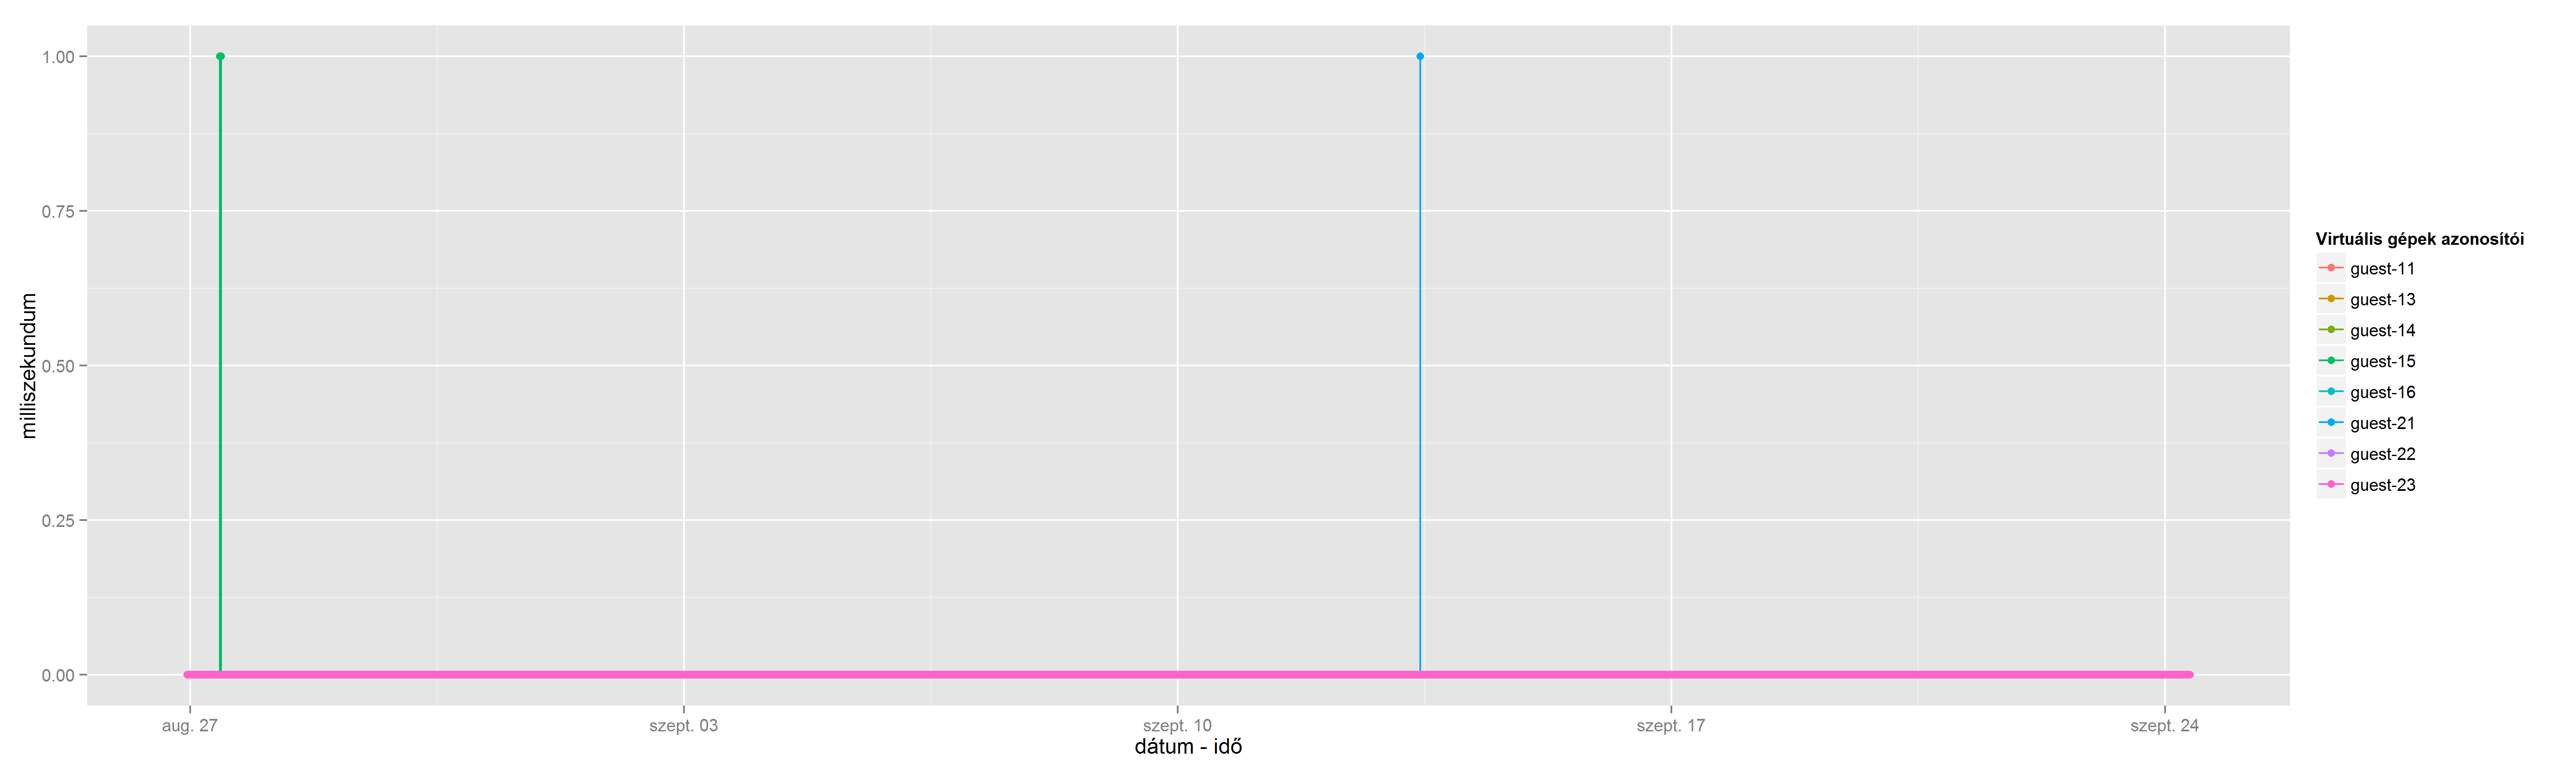
\includegraphics[width=1.00\textwidth]{figures/cpu_swapwait_summation-20120826230140-20120924083120.png}
\caption{A cpu.swapwait.summation értékei a monitorozott időintervallumban \label{fig:cpu_swapwait_summation}}
\end{figure}

\begin{figure}[h!]
\centering
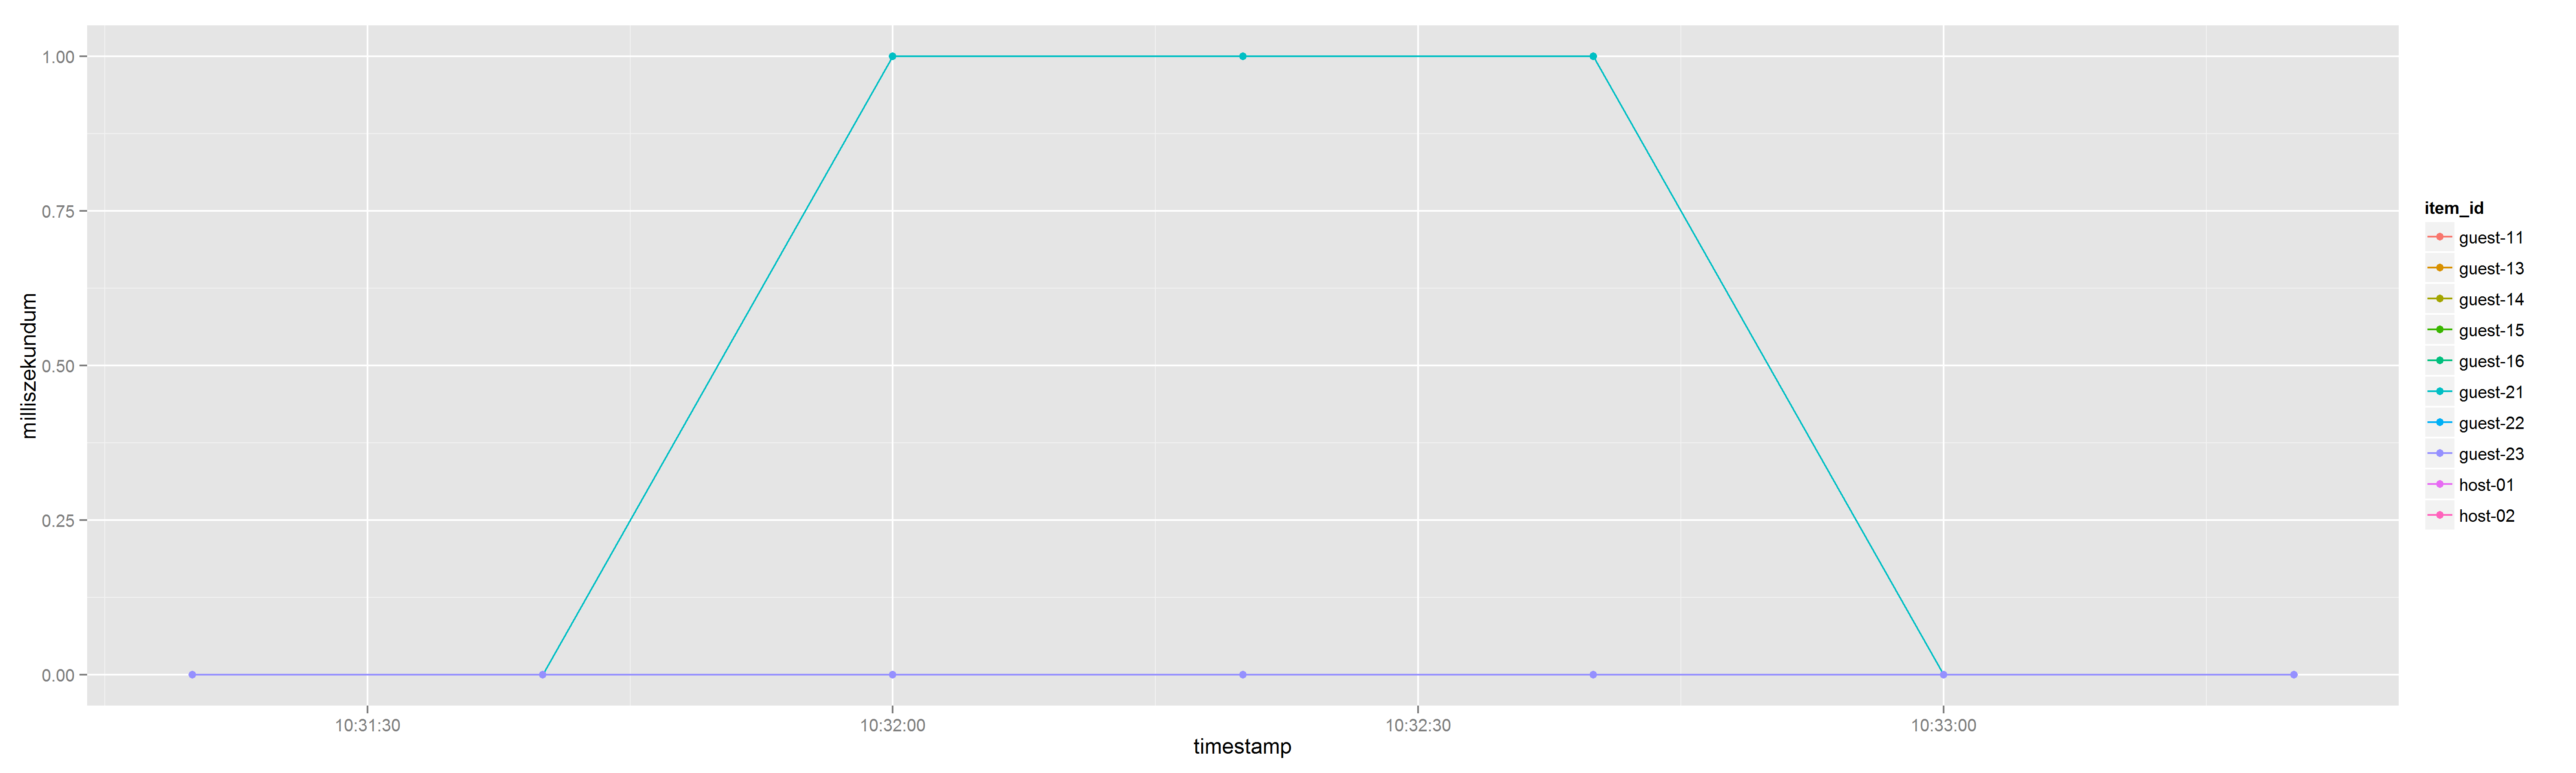
\includegraphics[width=1.00\textwidth]{figures/cpu_swapwait_summation-20120913103115-20120913103330.png}
\caption{A cpu.swapwait.summation értéke 2012.09.13. 10:31:15 - 10:33:30 között \label{fig:cpu_swapwait_summation_0913}}
\end{figure}

\begin{figure}[h!]
\centering
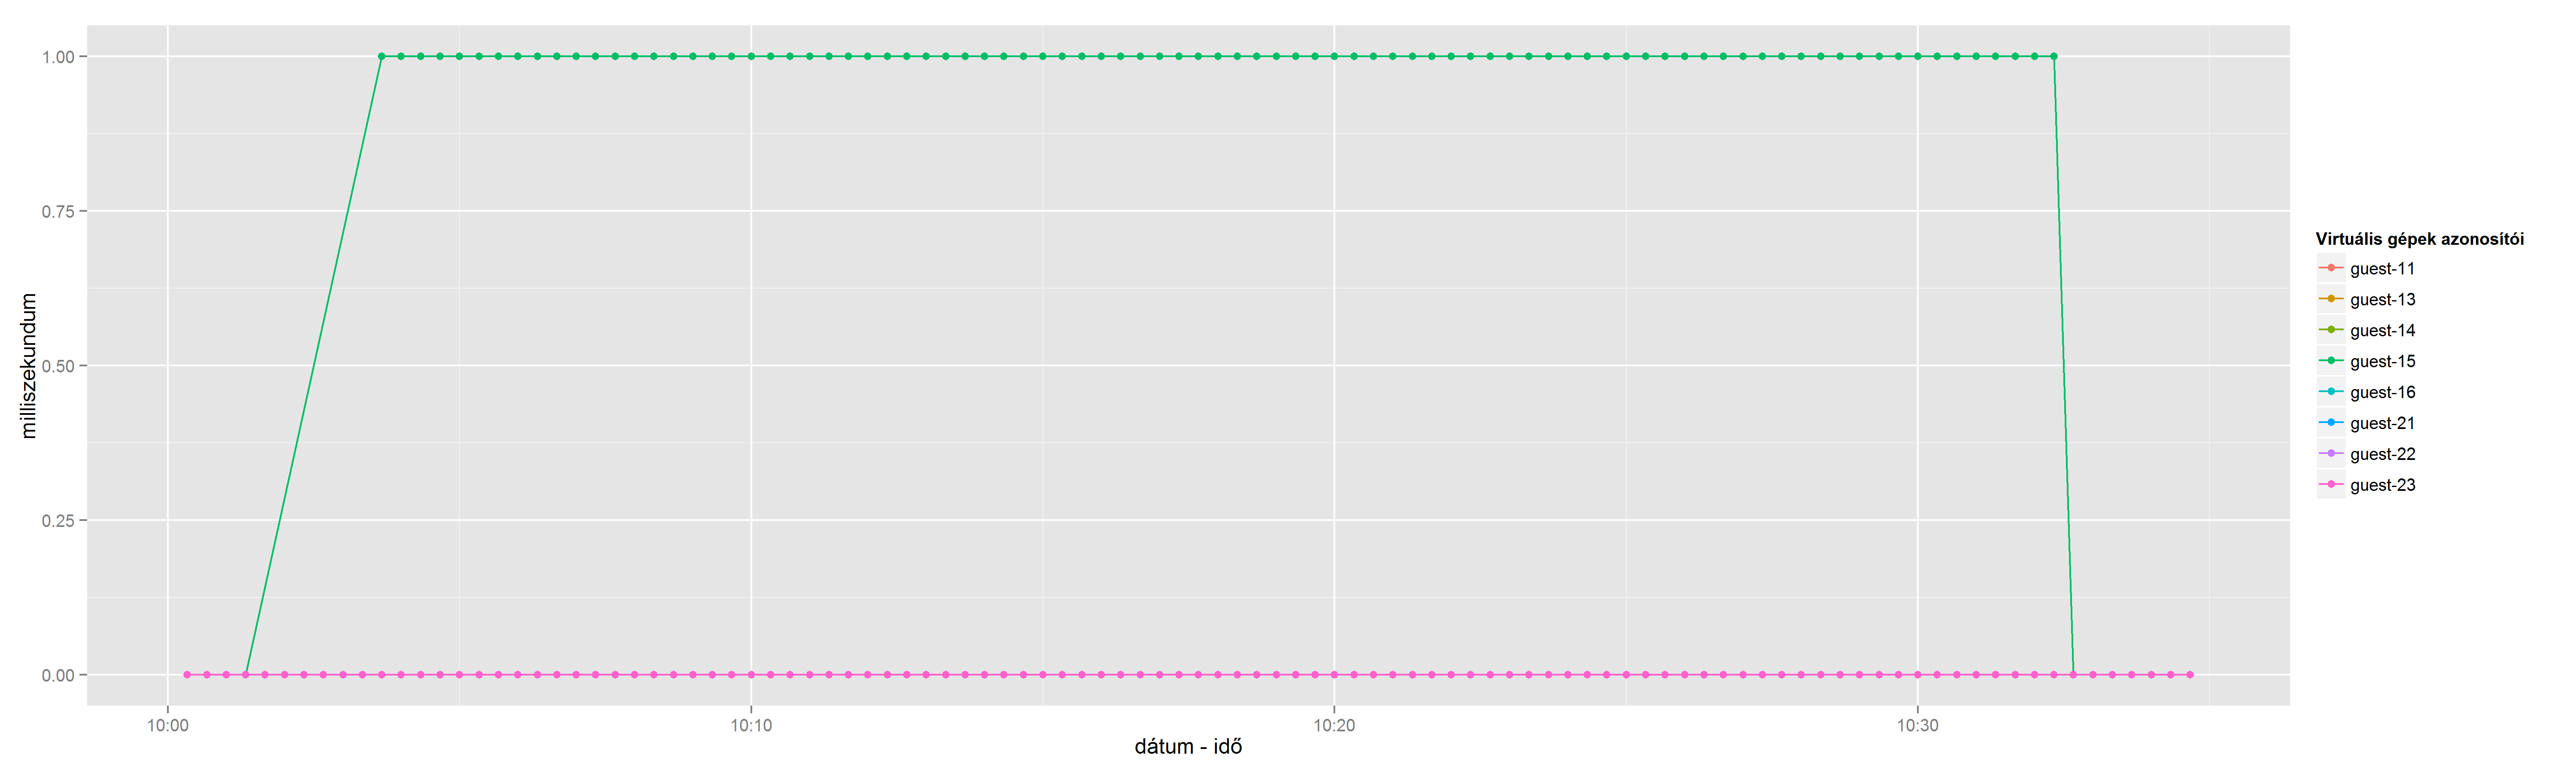
\includegraphics[width=1.00\textwidth]{figures/cpu_swapwait_summation-20120827100000-20120827103500.png}
\caption{A cpu.swapwait.summation értéke 2012.08.27. 10:00:00 - 10:35:00 között \label{fig:cpu_swapwait_summation_082701}}
\end{figure}

\begin{figure}[h!]
\centering
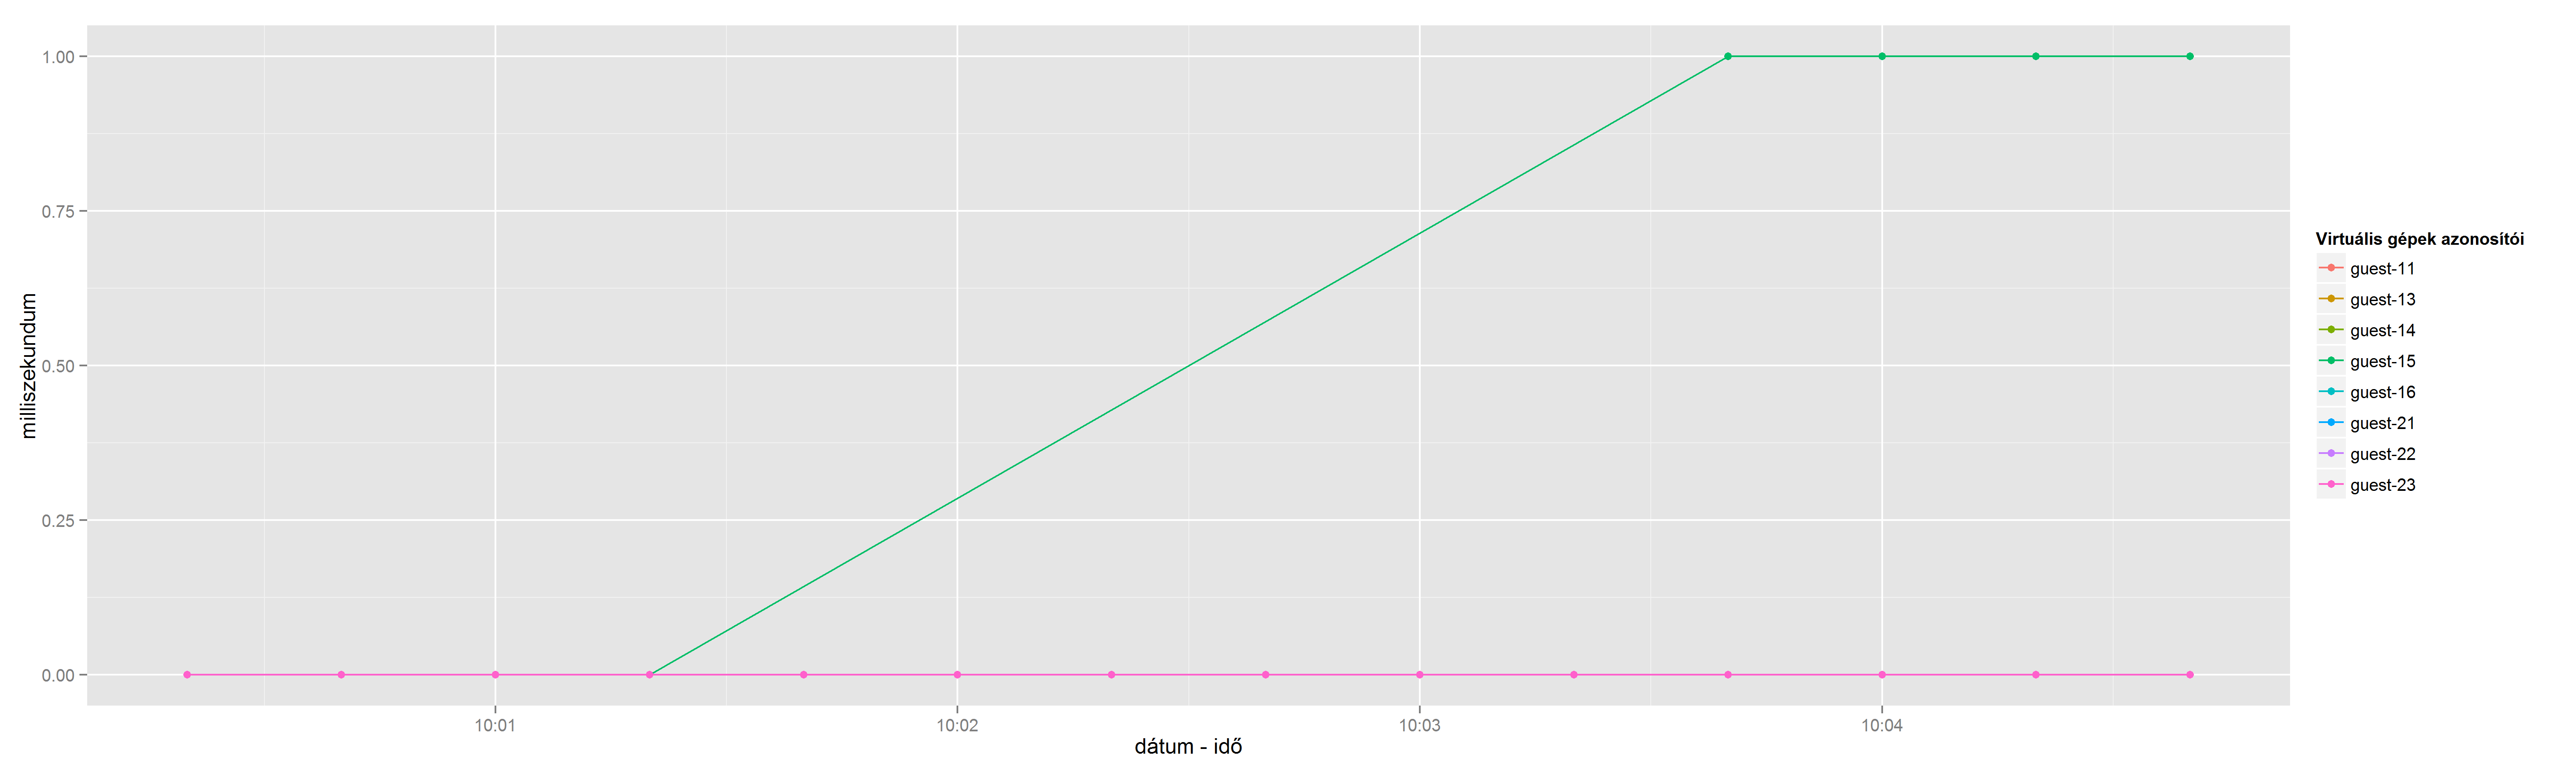
\includegraphics[width=1.00\textwidth]{figures/cpu_swapwait_summation-20120827100000-20120827100500.png}
\caption{A cpu.swapwait.summation értéke 2012.08.27. 10:00:00 - 10:05:00 között \label{fig:cpu_swapwait_summation_082702}}
\end{figure}
%#
%###############################################################################

%###############################################################################
%#
%#                    cpu.idle.summation
%#
\subsection{A cpu.idle.summation metrika}

Vizsgálódásunk tárgyai ebben az esetben a \textit{guest-15} és \textit{guest-16} nevű virtuális gépek. \Aref{fig:cpu_idle_summation_g16_1}.~ábrán a \textit{guest-16} VM idle értékei láthatóak a teljes mérési időben. Ahhoz, hogy követeztetéseket tudjunk levonni csökkentenünk kell az időablakot. \Aref{fig:cpu_idle_summation_g16_2}.~ábrával már egyszerűbb dolgunk van. \Aref{fig:cpu_idle_summation_g16_1}.~ábra tömörségének oka, hogy egyfajta periodicitás jellemzi a VM idle állapotban töltött idejét. 

\begin{figure}[h!]
\centering
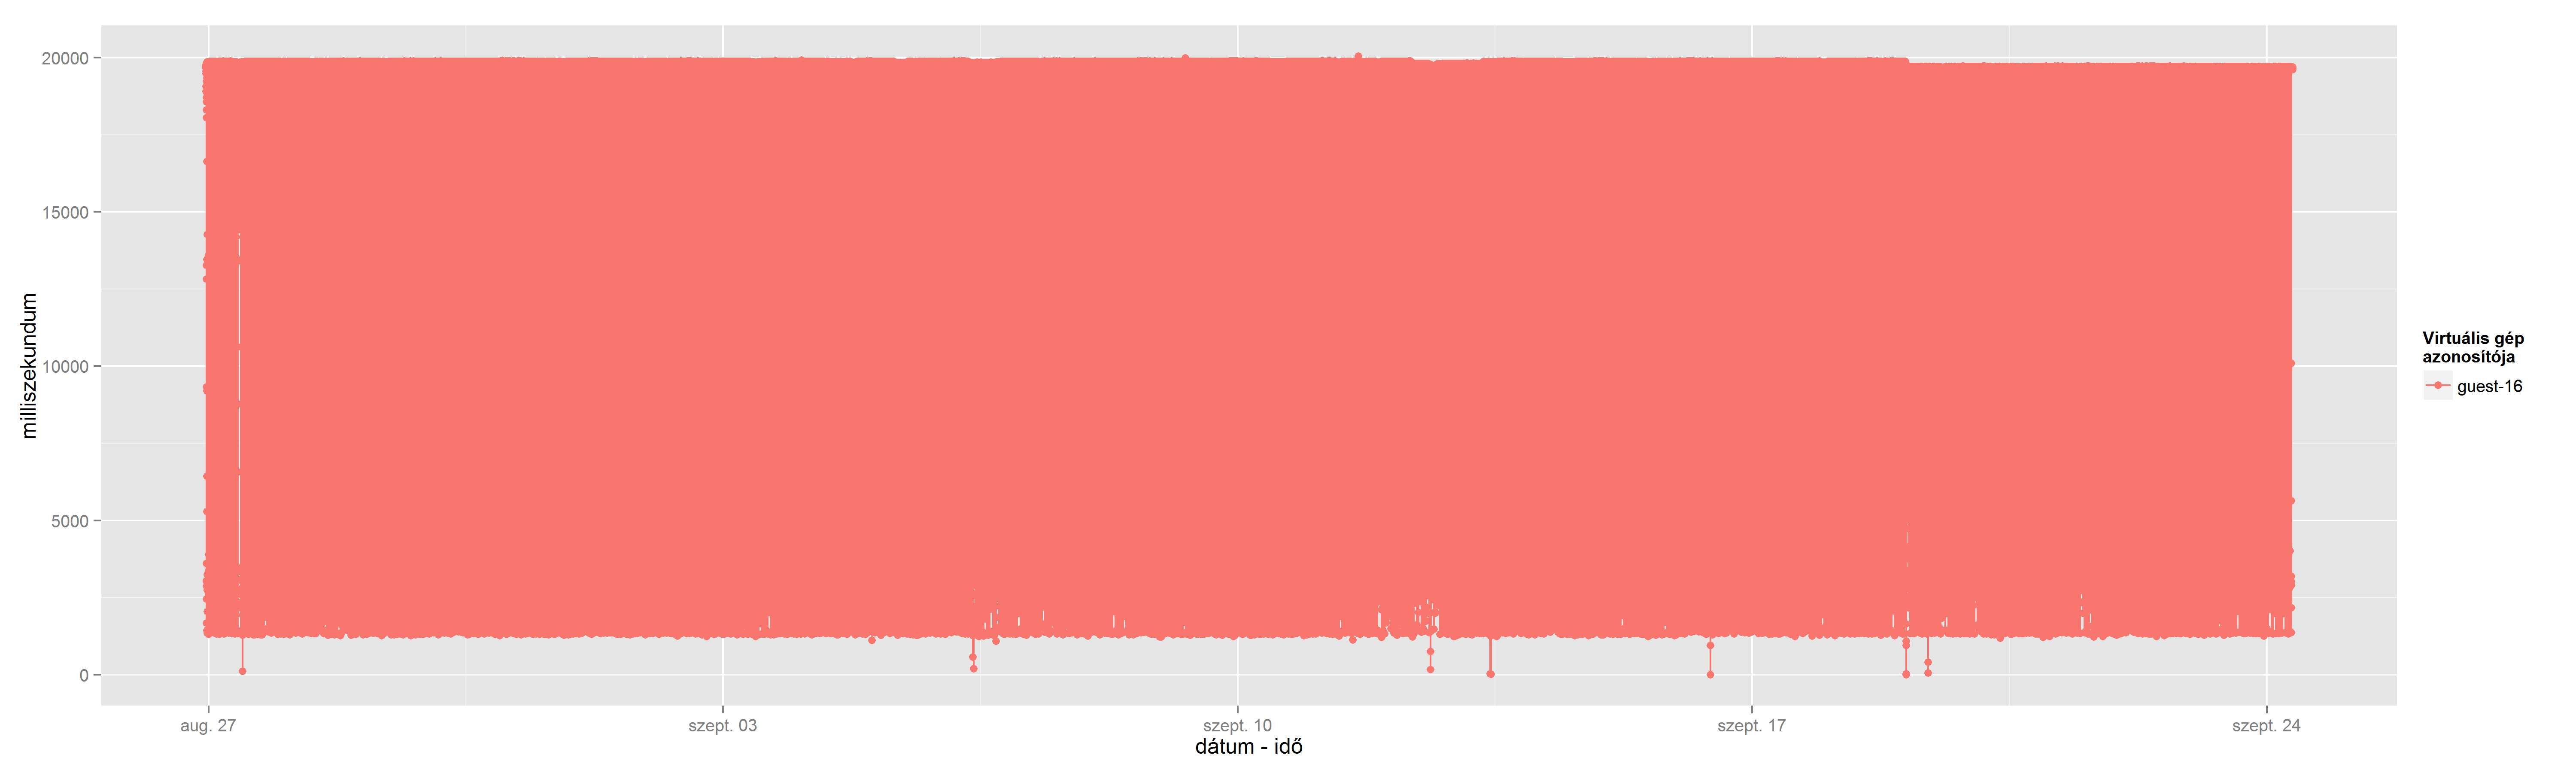
\includegraphics[width=1.00\textwidth]{figures/cpu_idle_summation-guest-16-20120826230140-20120924083120.png}
\caption{A guest-16 VM cpu.idle.summation értéke a monitorozott időintervallumban \label{fig:cpu_idle_summation_g16_1}}
\end{figure}

\begin{figure}[h!]
\centering
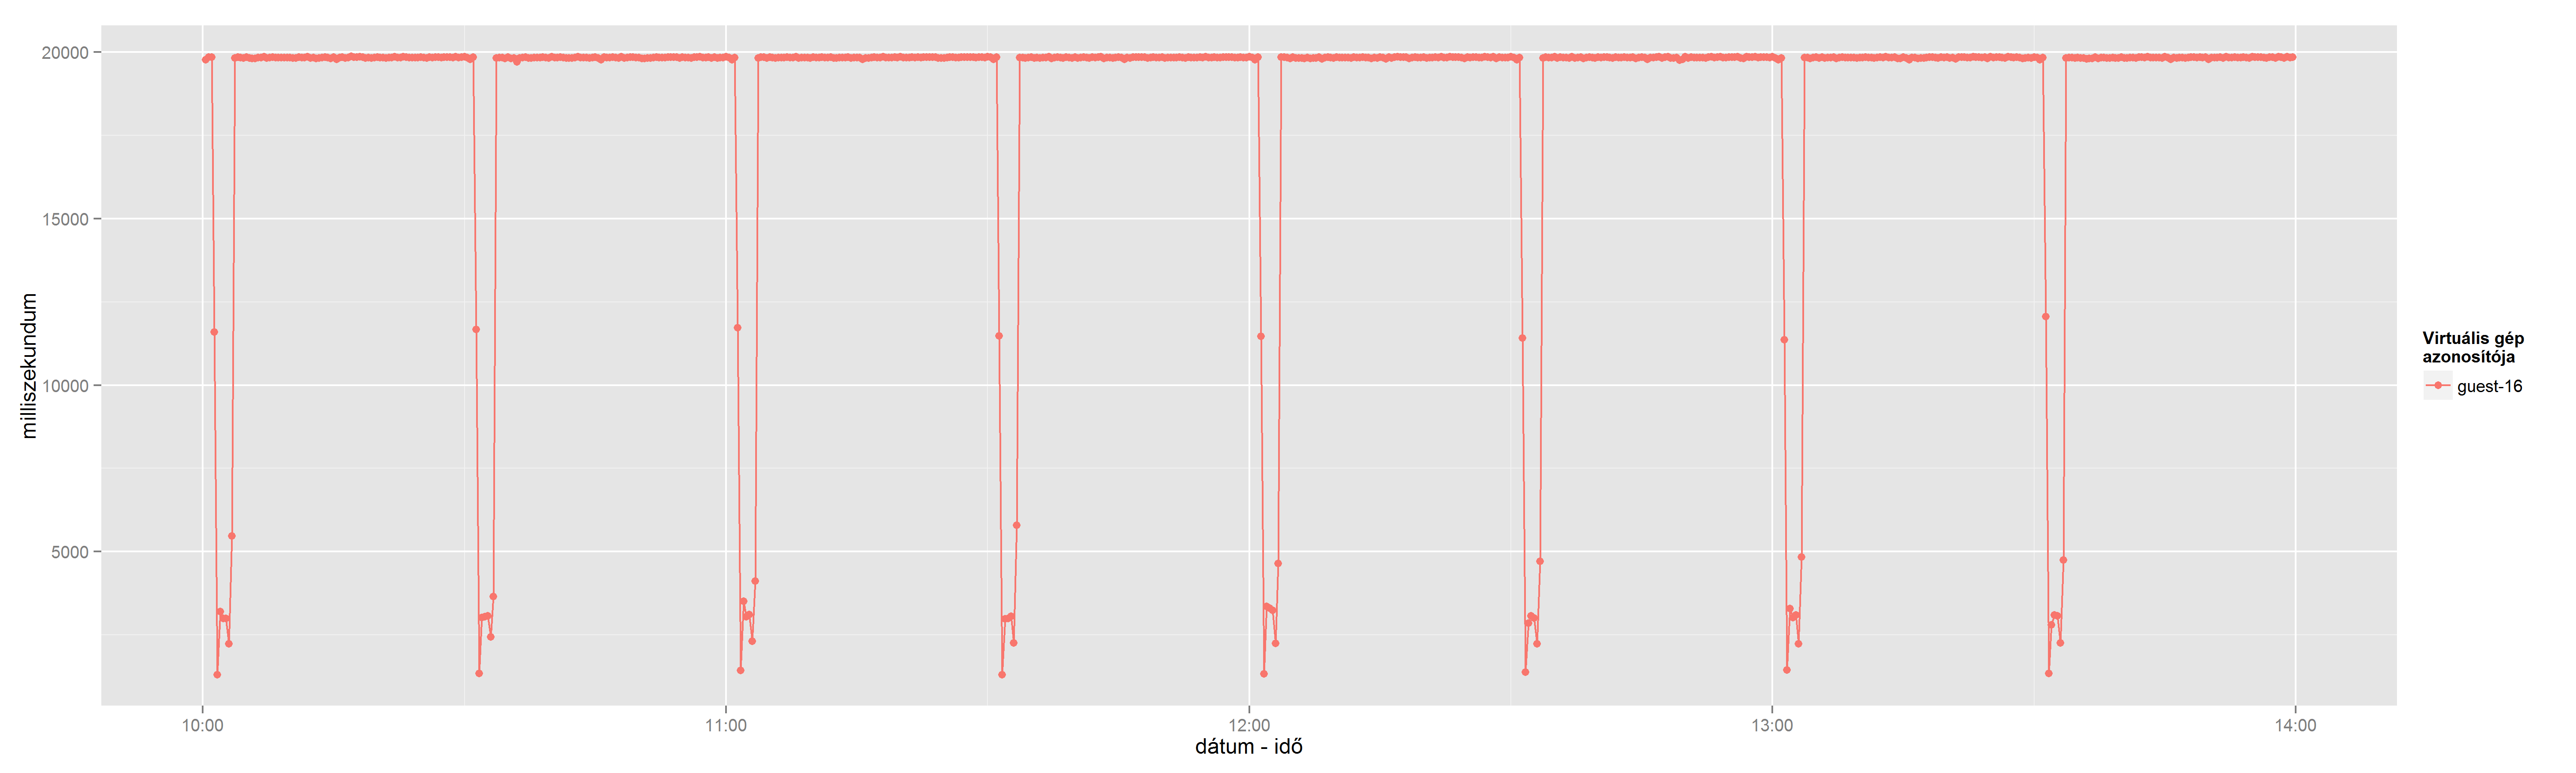
\includegraphics[width=1.00\textwidth]{figures/cpu_idle_summation-guest-16-20120910100000-20120910140000.png}
\caption{A guest-16 VM cpu.idle.summation értéke 2012.09.10. 10:00:00 és 2012.09.10. 14:00:00 között \label{fig:cpu_idle_summation_g16_2}}
\end{figure}

A \textit{guest-15} nevű virtuális gép \texttt{cpu.idle.summation} grafikonja jó példa arra, hogy a vizuális adatelemzés segítségével könnyen kiszúrhatjuk az esetleges mérési hibákat. \Aref{fig:cpu_idle_summation_g15_1}.~ábrán látható, hogy két esetben is (20000 milliszekundumnál) nagyobb értékek találhatóak az adathalmazunkban, mint ahogy annak értelme lenne. \Aref{fig:cpu_idle_summation_g15_2}.~ábra kisebb időablakban mutatja az egyik mérési hiba megjelenését.

\begin{figure}[h!]
\centering
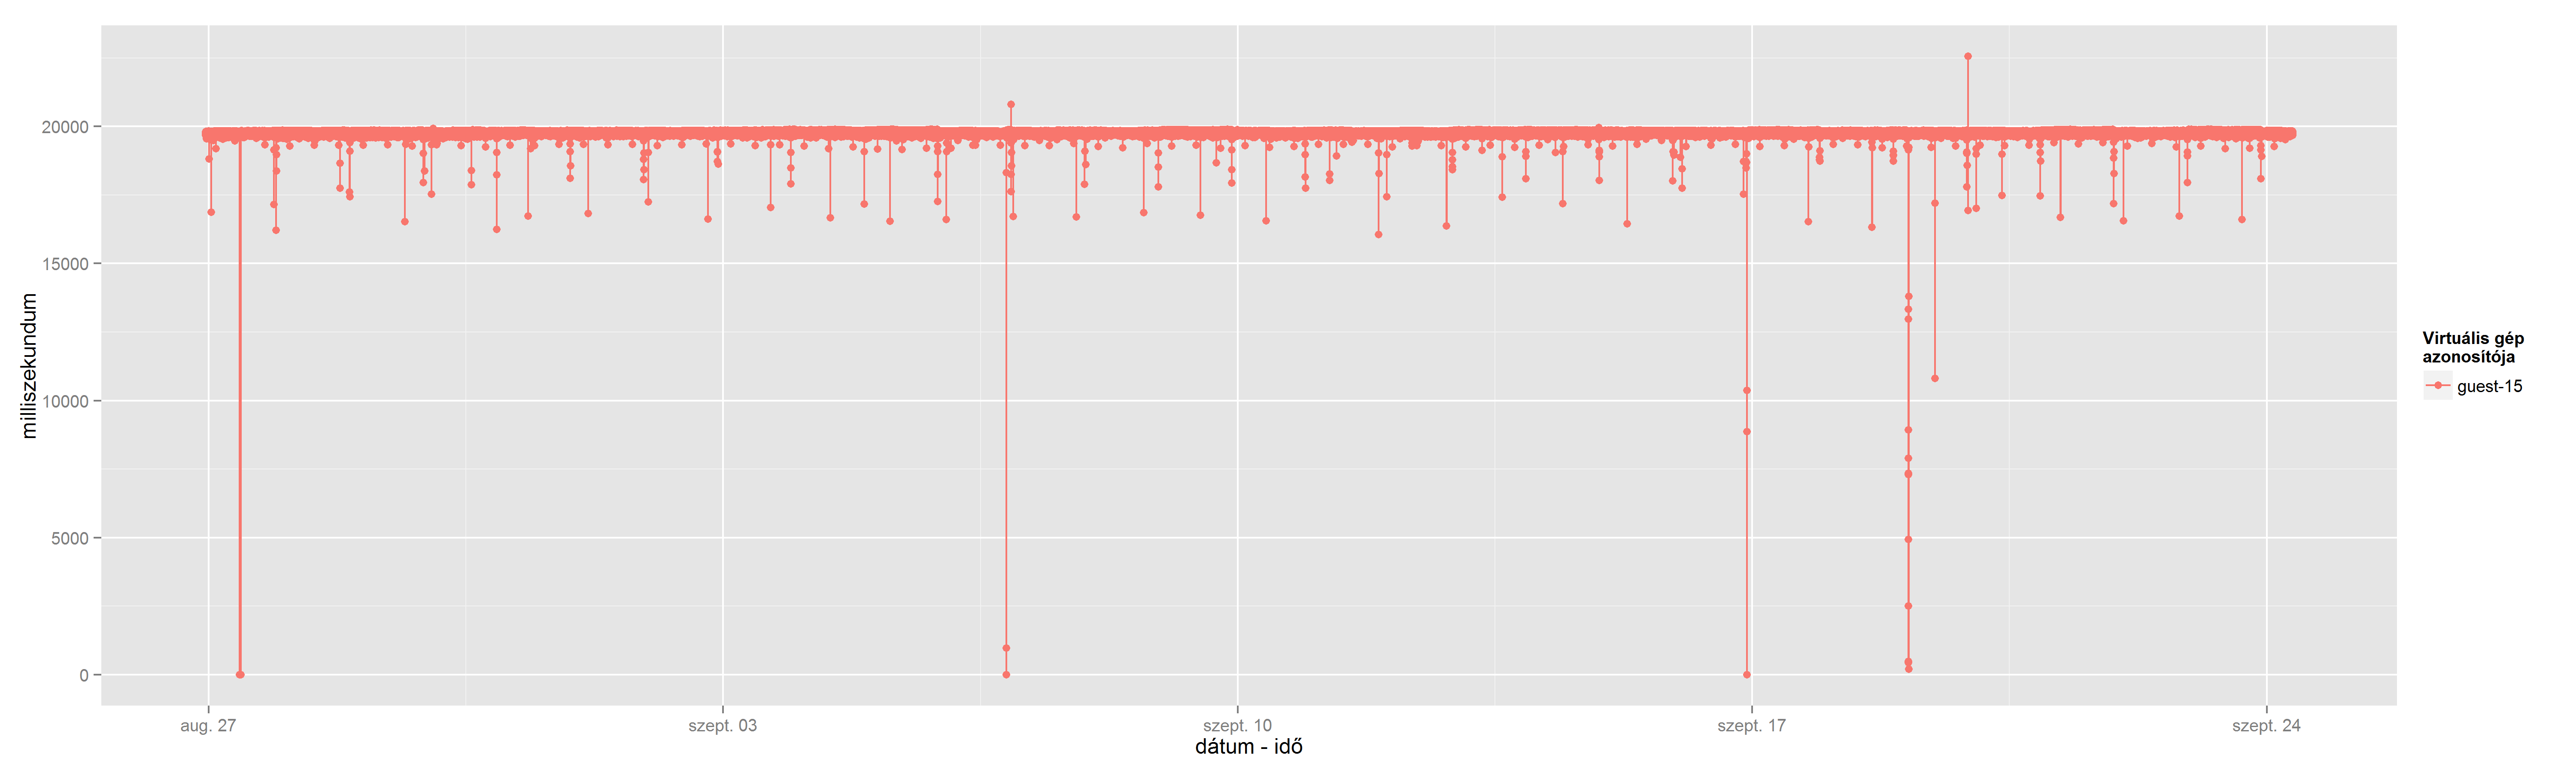
\includegraphics[width=1.00\textwidth]{figures/cpu_idle_summation-guest-15-20120826230140-20120924083120.png}
\caption{A guest-15 VM cpu.idle.summation értéke a monitorozott időintervallumban \label{fig:cpu_idle_summation_g15_1}}
\end{figure}

\begin{figure}[h!]
\centering
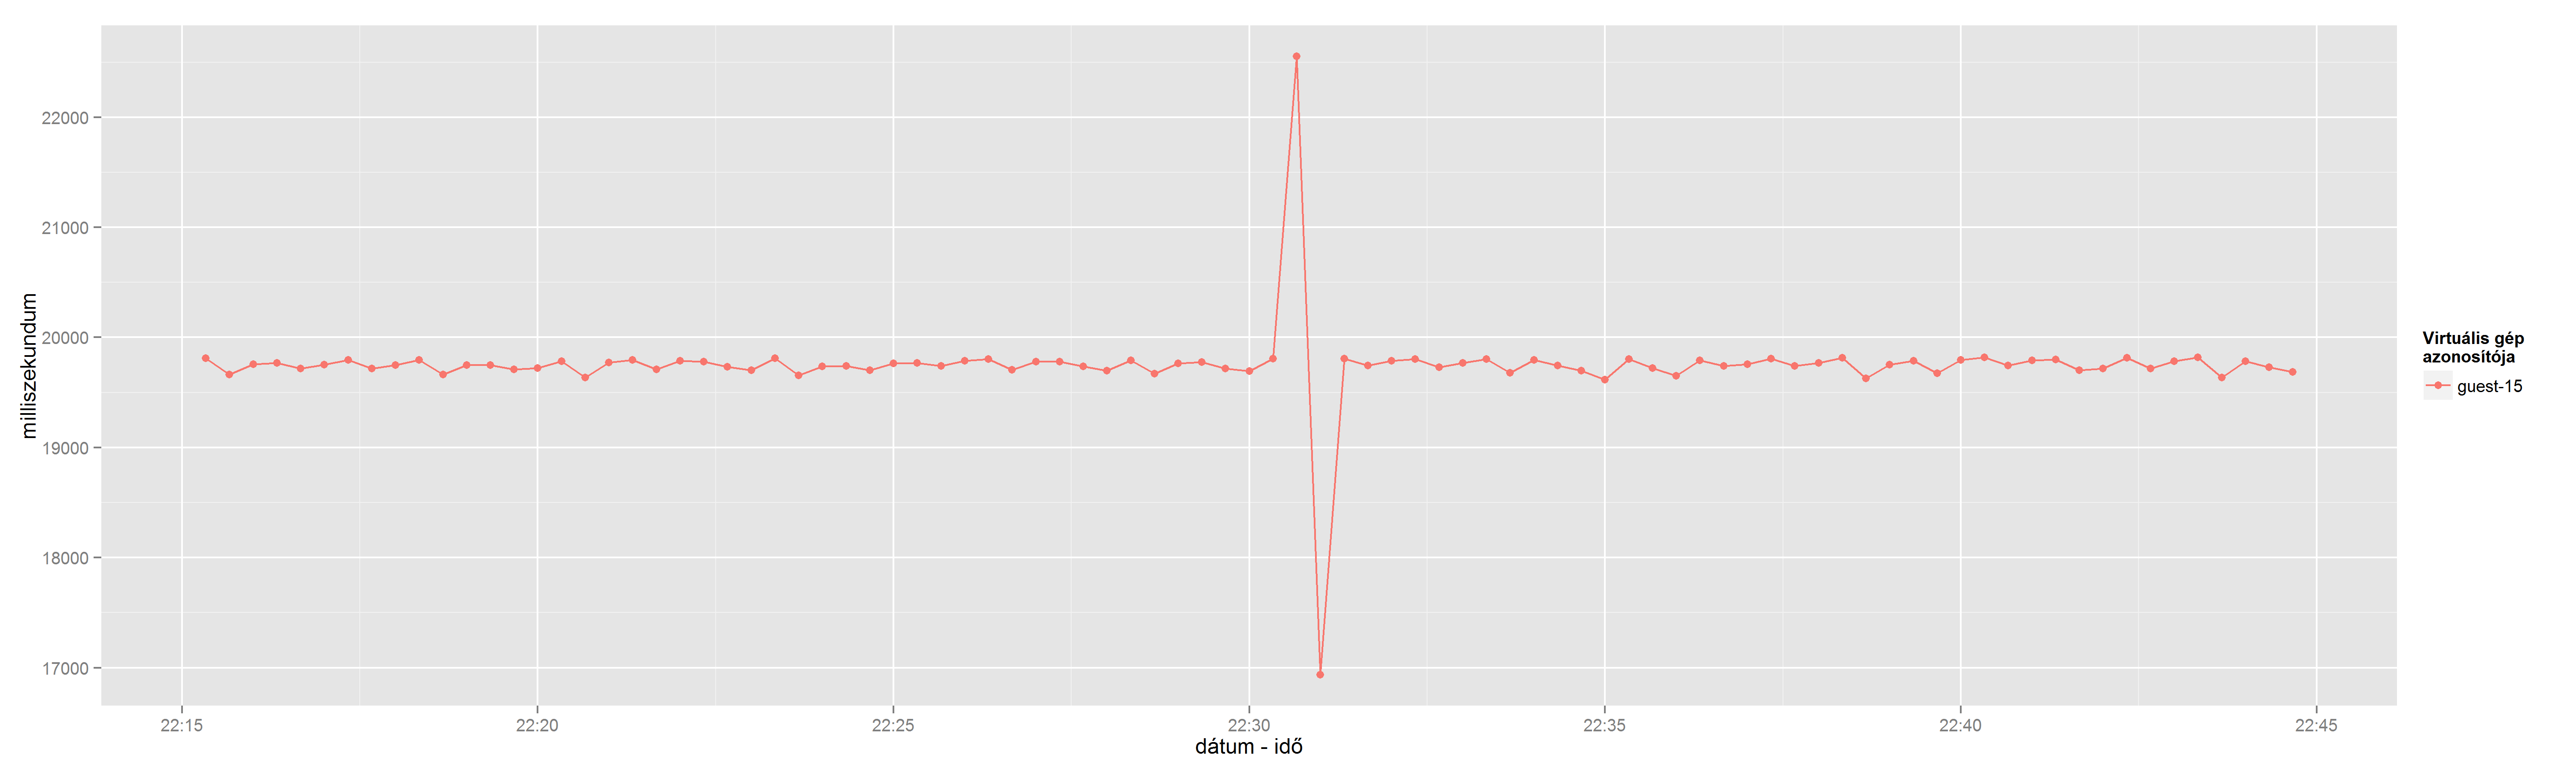
\includegraphics[width=1.00\textwidth]{figures/cpu_idle_summation-guest-15-20120919221500-20120919224500.png}
\caption{A guest-15 VM cpu.idle.summation értéke 2012.09.19. 22:15:00 és 2012.09.19. 22:45:00 között \label{fig:cpu_idle_summation_g15_2}}
\end{figure}

\begin{figure}[h!]
\centering
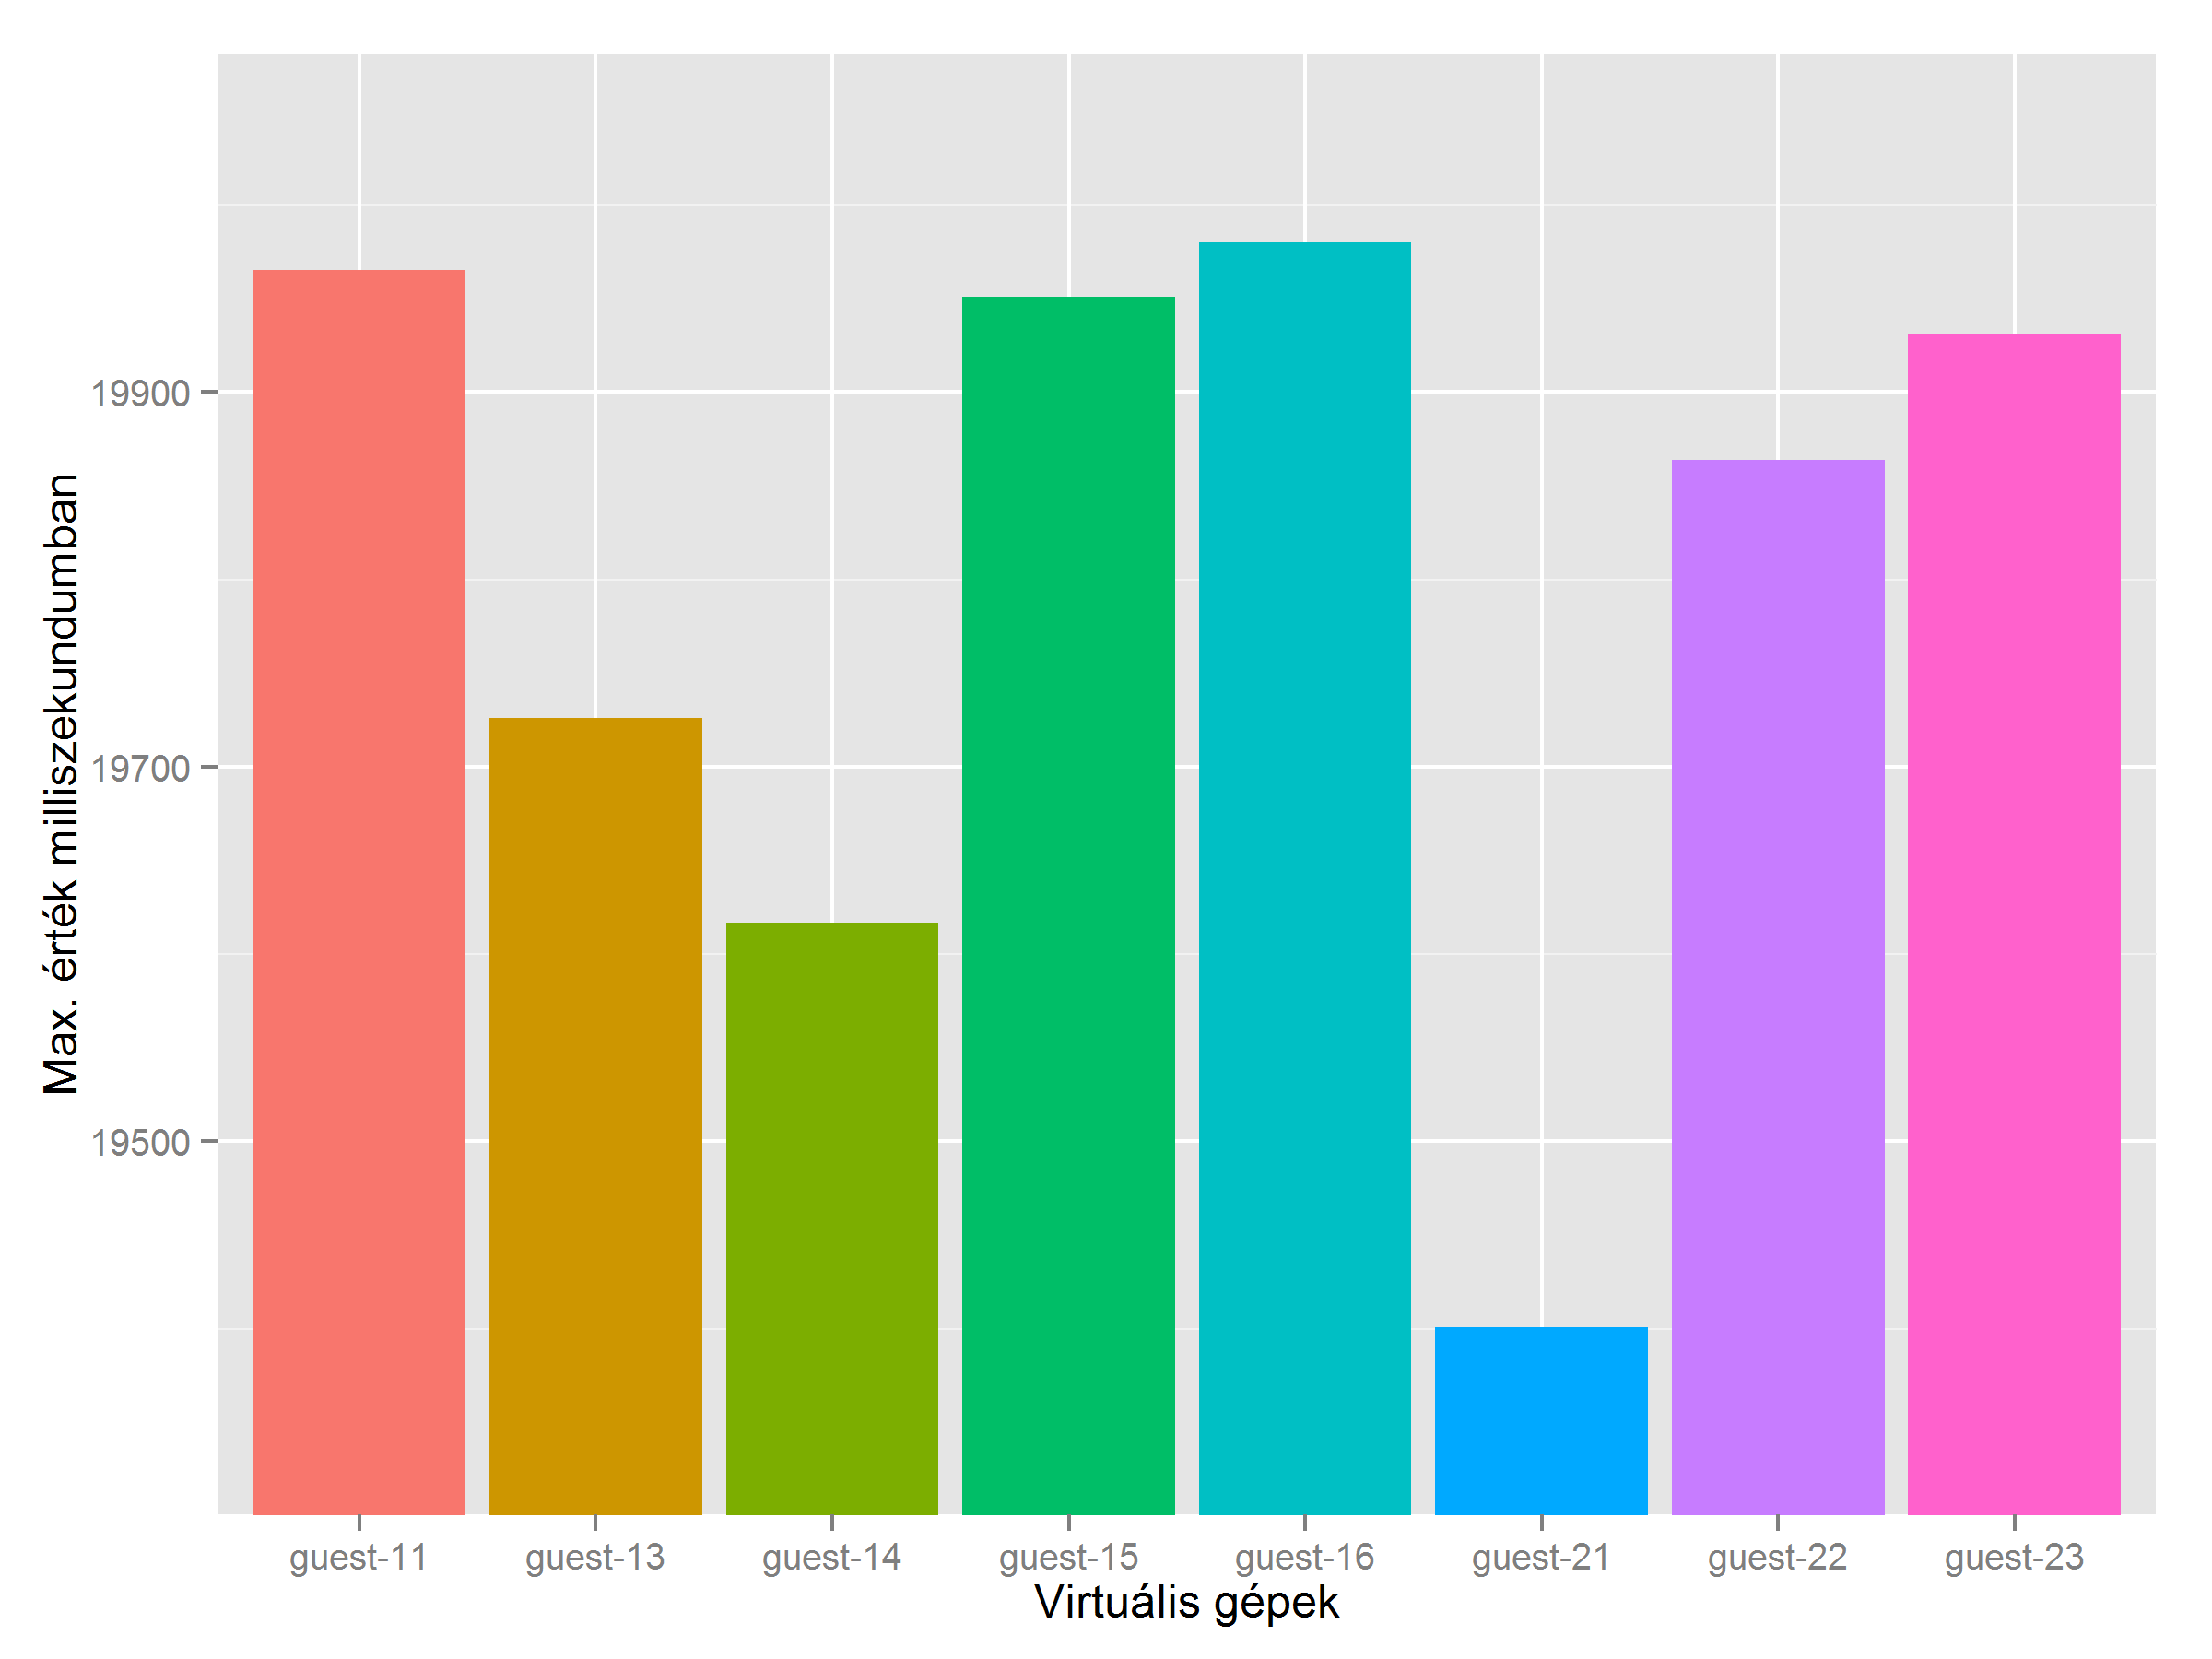
\includegraphics[width=1.00\textwidth]{figures/cpu_idle_summation-max-barchart.png}
\caption{Az egyes VM-ek max. cpu.idle.summation értéke a teljes megfigyelési időintervallumra nézve \label{fig:cpu_idle_summation_max_barchart}}
\end{figure}

Érdemes megnézni az egyes virtuális gépek idle állapotban eltöltött idejének maximumát. Ezt mutatja \aref{fig:cpu_idle_summation_max_barchart}.~ábra.

\mycomment{A már említett mérési hibák nem jelennek meg \aref{fig:cpu_idle_summation_max_barchart}.~ábrán, azok eltávolításra kerültek a diagram adathalmazából.}
%#
%###############################################################################

%###############################################################################
%#
%#                    A cpu.ready.summation metrika:
%#
\subsection{A cpu.ready.summation metrika}

A cpu.ready.summation metrika az egyik legismertebb teljesítmény indikátor a metrikák közül. Amennyiben egy virtuális gép futásra kész állapotban van, ám ennek ellenére nem jut fizikai processzor időhöz, úgy ennek a számlálónak az értéke növekszik, maximum a 20 másodperces mintavételezési ablak értékéig.

Amennyiben egy virtuális infrastruktúra monitorozása során magas CPU ready értékeket figyelünk meg, úgy abban az esetben érdemes utána járni, hogy mi lehet ennek az oka. Általában ha túlterhelt (sok VM-et működtet) a kiszolgálónk, az megjelenik a magas ready időkben \cite{link:VPM}.

Magas értékekről beszélünk, ha a ready meghaladja az időablak 10\%-át, tehát 2 másodpercet. Egy átlagos kihasználtsággal rendelkező infrastruktúra esetében a ready értékek 5\% környékiek \cite{link:CRT}.

A \textit{guest-13} azonosítójú VM ready értékeit mutatja \aref{fig:cpu_ready_summation_g13}.~ábra. Megfigyelhető, hogy a legmagasabb érték sem éri el a 150 milliszekundum körüli értéket, de sok esetben 20 milliszekundum körüli.

\begin{figure}[h!]
\centering
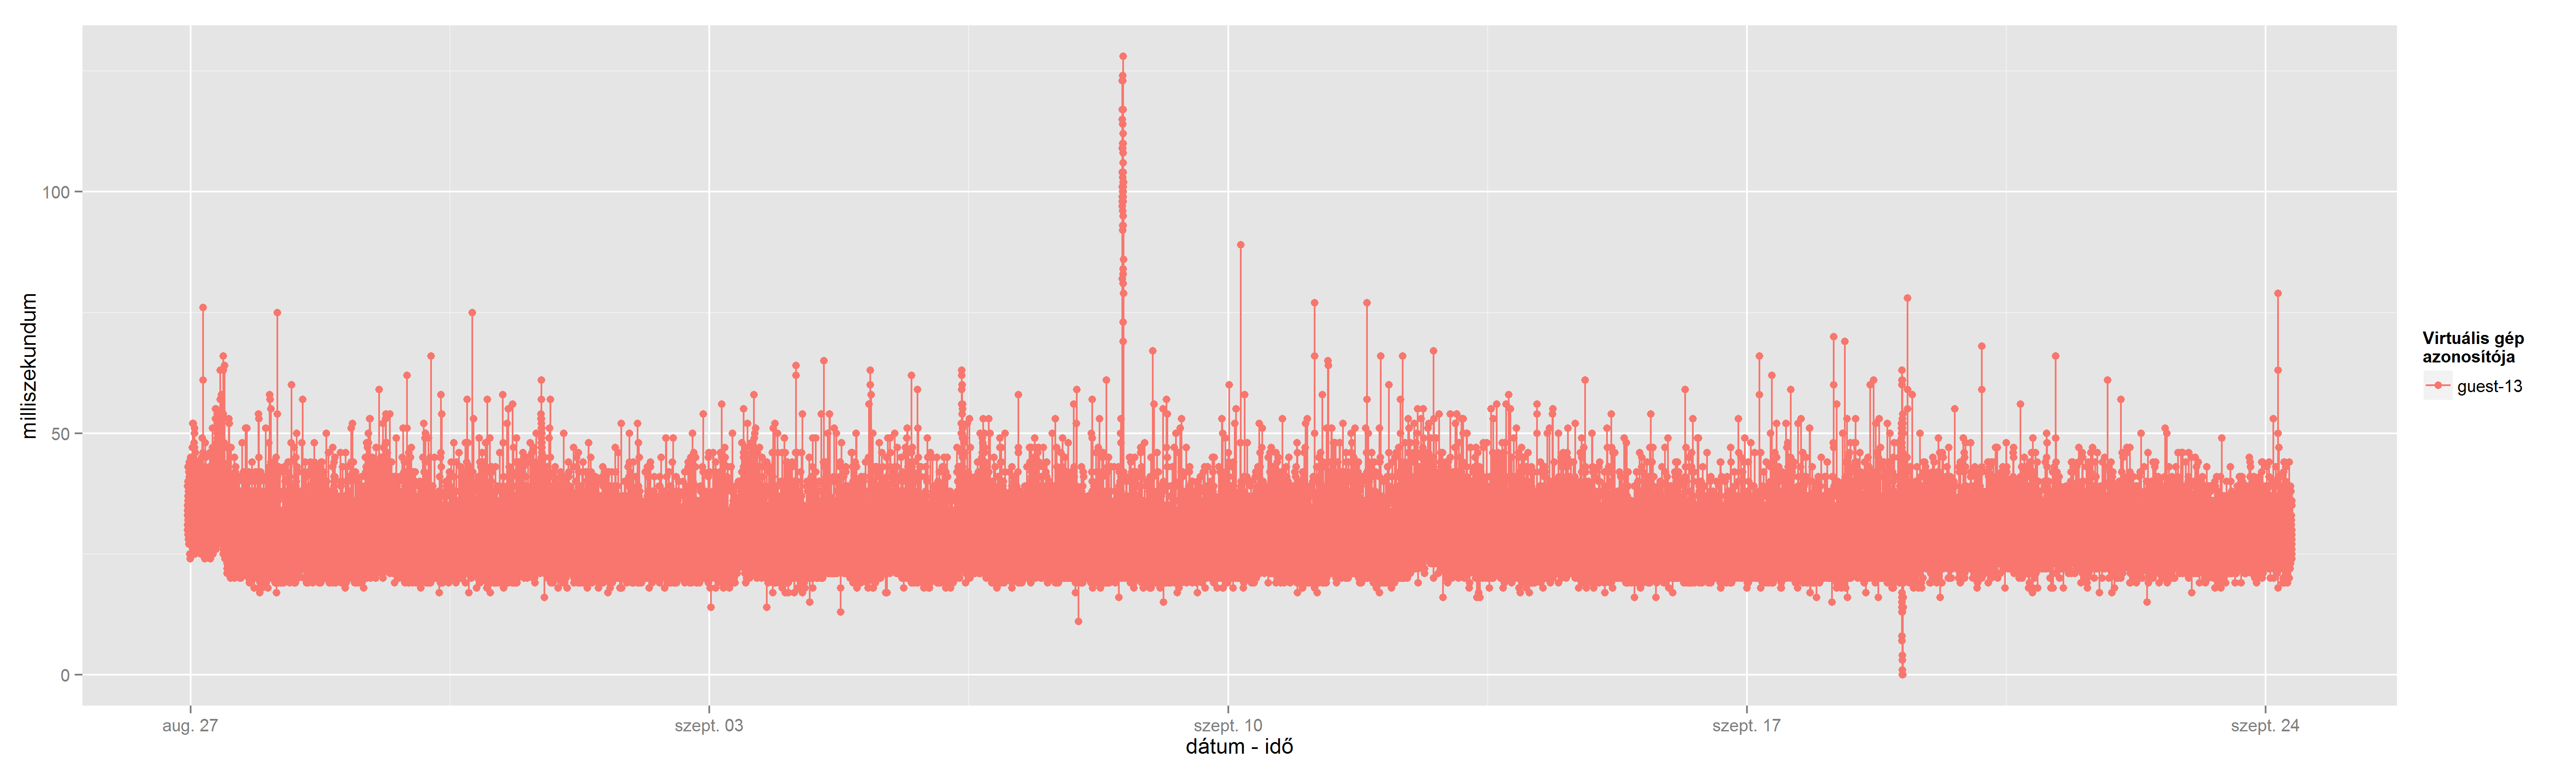
\includegraphics[width=1.00\textwidth]{figures/cpu_ready_summation-guest-13-20120826230140-20120924083120.png}
\caption{A cpu.ready.summation alakulása a guest-13 azonosítójú VM esetében a teljes megfigyelési időintervallumon \label{fig:cpu_ready_summation_g13}}
\end{figure}

Érdekesebb lehet a \textit{guest-24} nevű virtuális gép (\ref{fig:cpu_ready_summation_g24_1}. és \ref{fig:cpu_ready_summation_g24_2}.~ábrák), hiszen ez 2 db virtuális CPU-val (vCPU) rendelkezik. Az ilyen virtuális gépek esetében eltérő ütemezési stratégiát alkalmaznak, hogy a vCPU-k belső órája ne csússzon szét egymáshoz és a fizikai CPU-hoz képest, ezért nagyobb ready értékek tapasztalhatóak \cite{link:VMCS}.

\begin{figure}[h!]
\centering
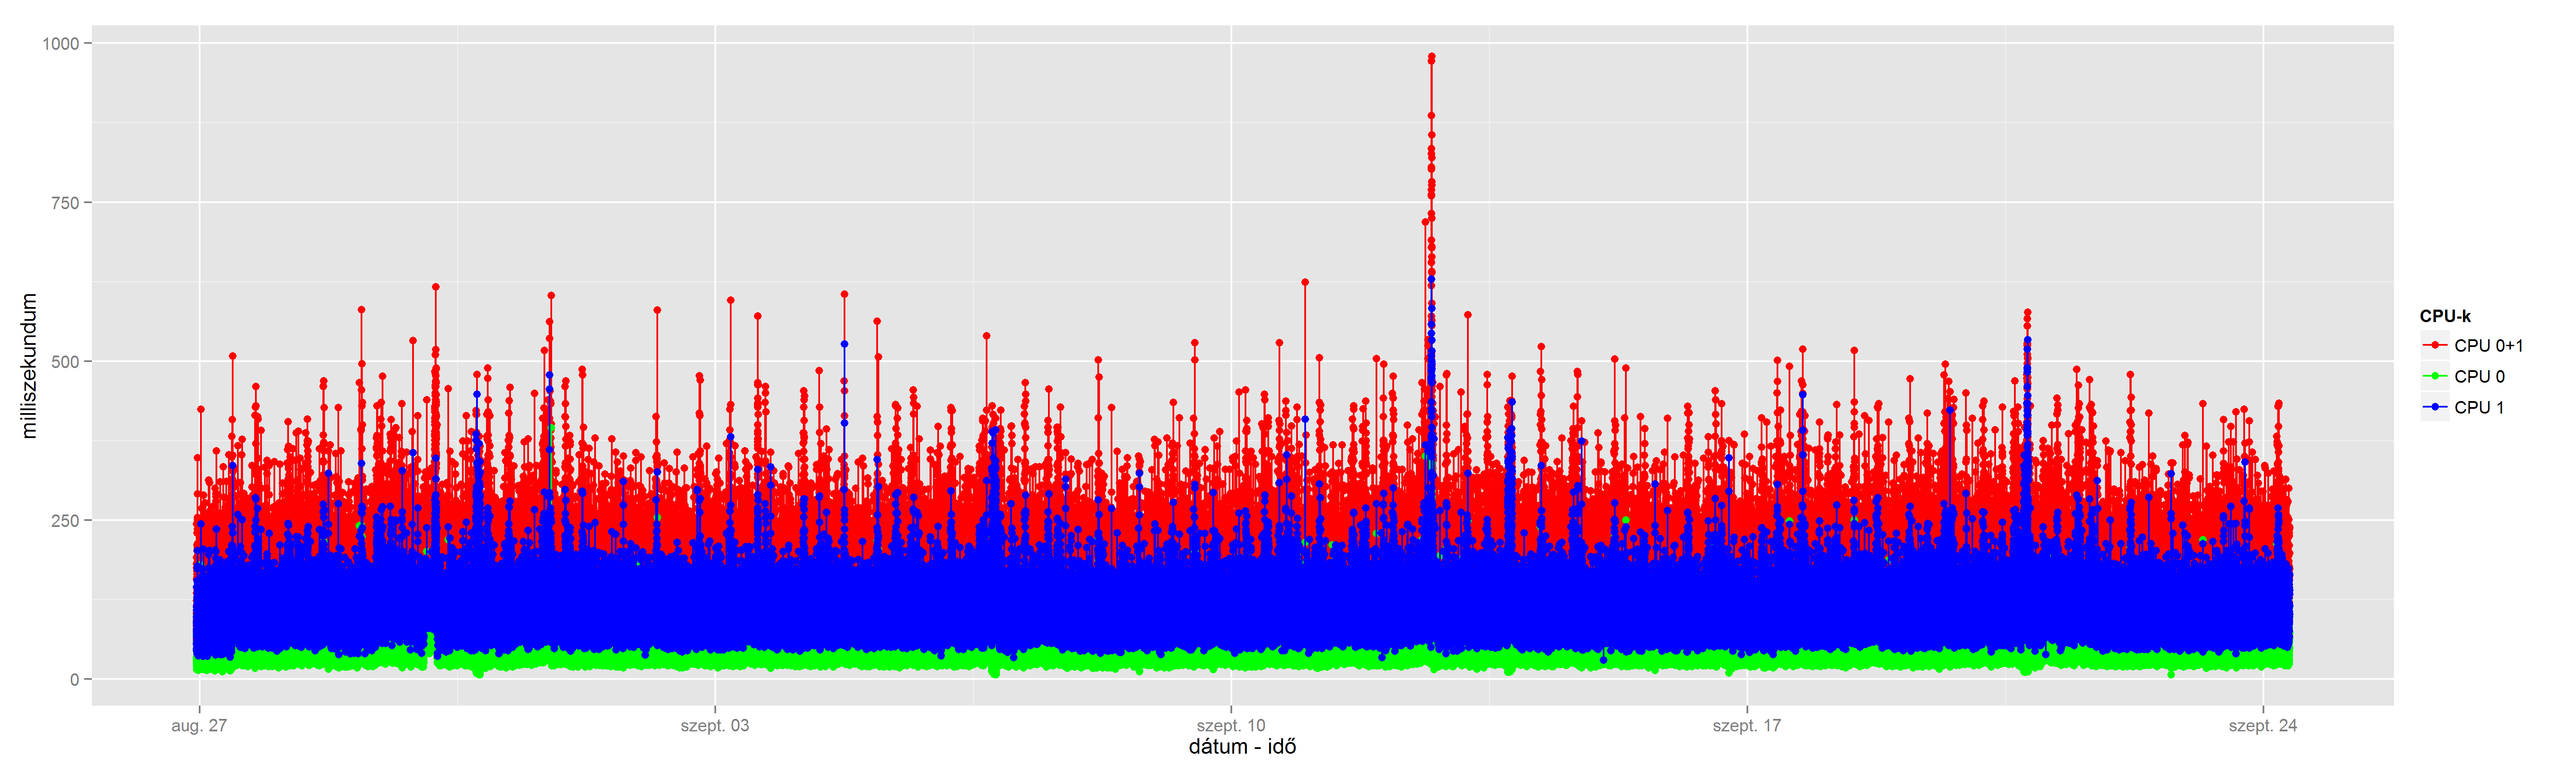
\includegraphics[width=1.00\textwidth]{figures/cpu_ready_summation-guest-24-20120826230140-20120924083120.png}
\caption{A cpu.ready.summation alakulása a guest-24 azonosítójú VM esetében a teljes megfigyelési időintervallumon \label{fig:cpu_ready_summation_g24_1}}
\end{figure}

\begin{figure}[h!]
\centering
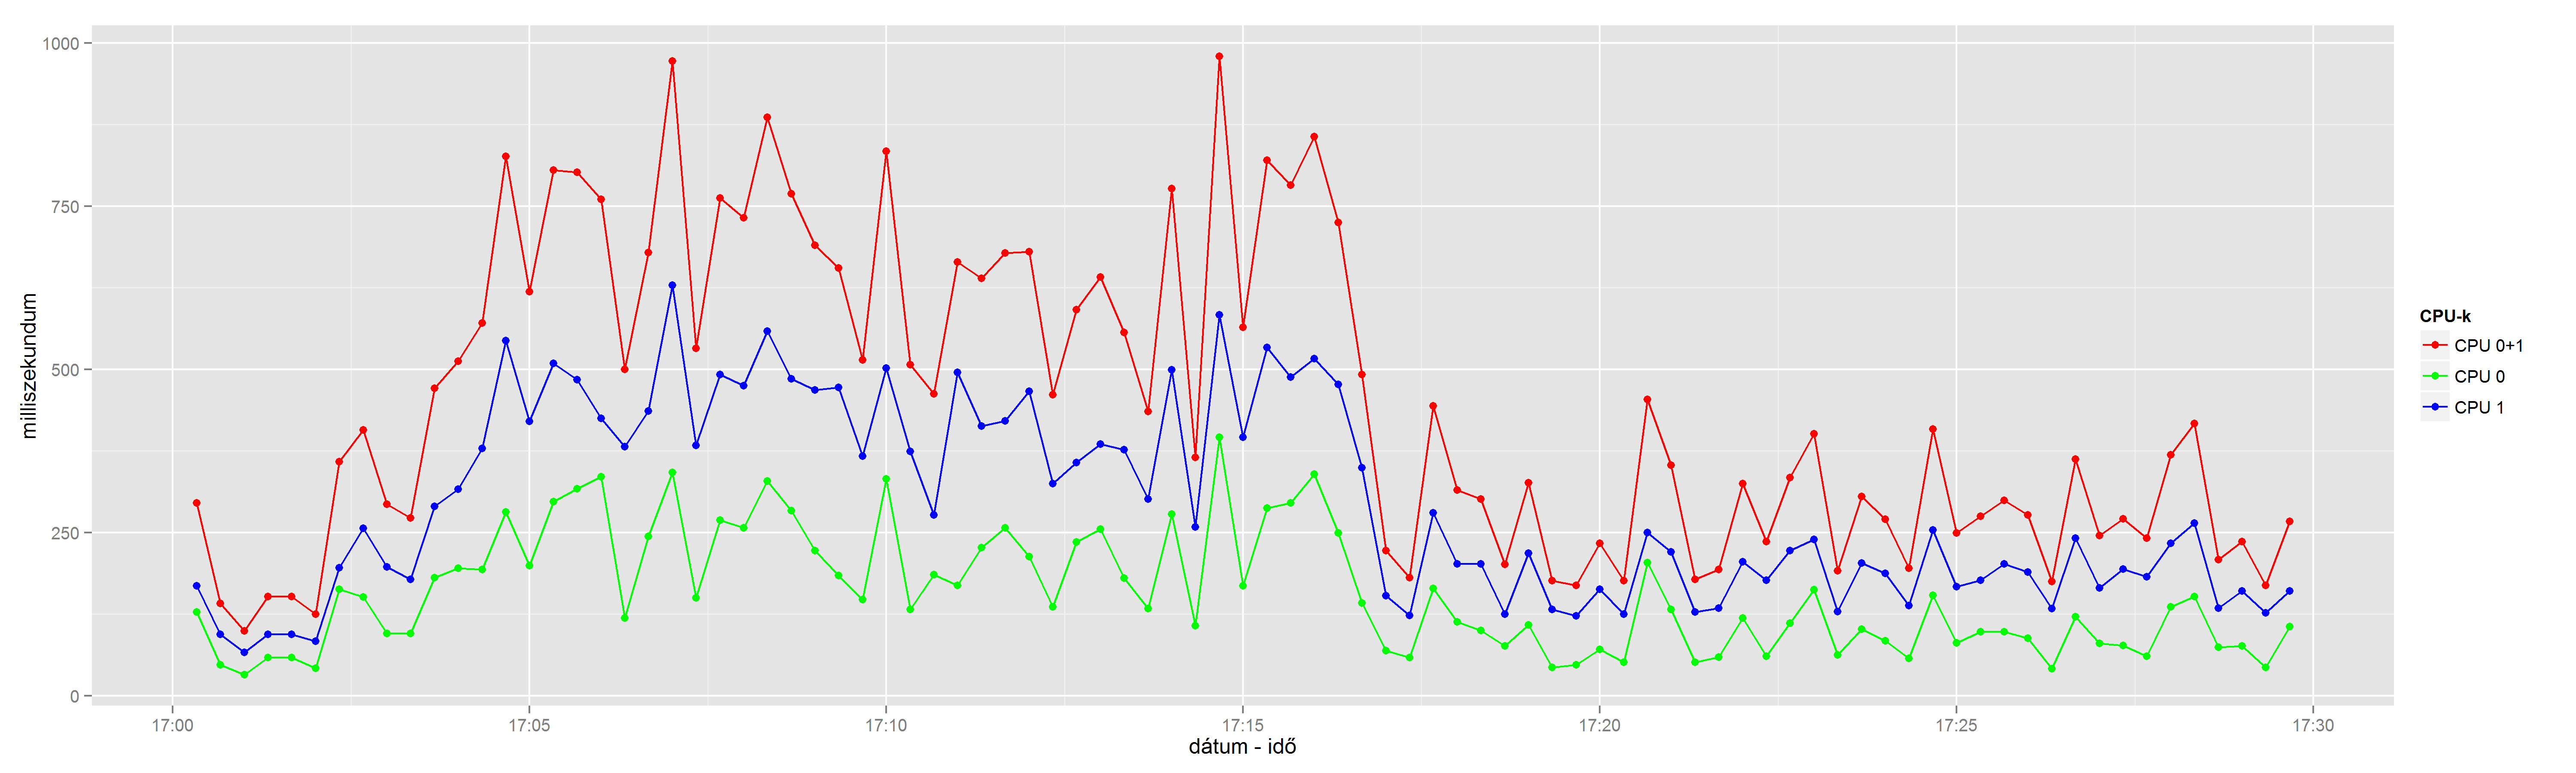
\includegraphics[width=1.00\textwidth]{figures/cpu_ready_summation-guest-24-20120912170000-20120912173000.png}
\caption{A cpu.ready.summation alakulása a guest-24 azonosítójú VM esetében 2012.09.12. 17:00:00 és 2012.09.12. 17:30:00 között \label{fig:cpu_ready_summation_g24_2}}
\end{figure}

\mycomment{Érdemes lehet megvizsgálni, hogy a vCPU-k ready értékeinek összege kiadja-e az összesített ready értéket, hiszen ebben az esetben az összesített metrika megfigyelése és tárolása felesleges lehet a redundáns információ tartalom miatt.}

\Aref{fig:cpu_ready_summation_max_barchart}.~ábrán az egyes virtuális gépek maximális CPU ready értékeit láthatjuk összesítve, a \textit{guest-24} esetében külön és összesítve is a vCPU-kra.

\begin{figure}[h!]
\centering
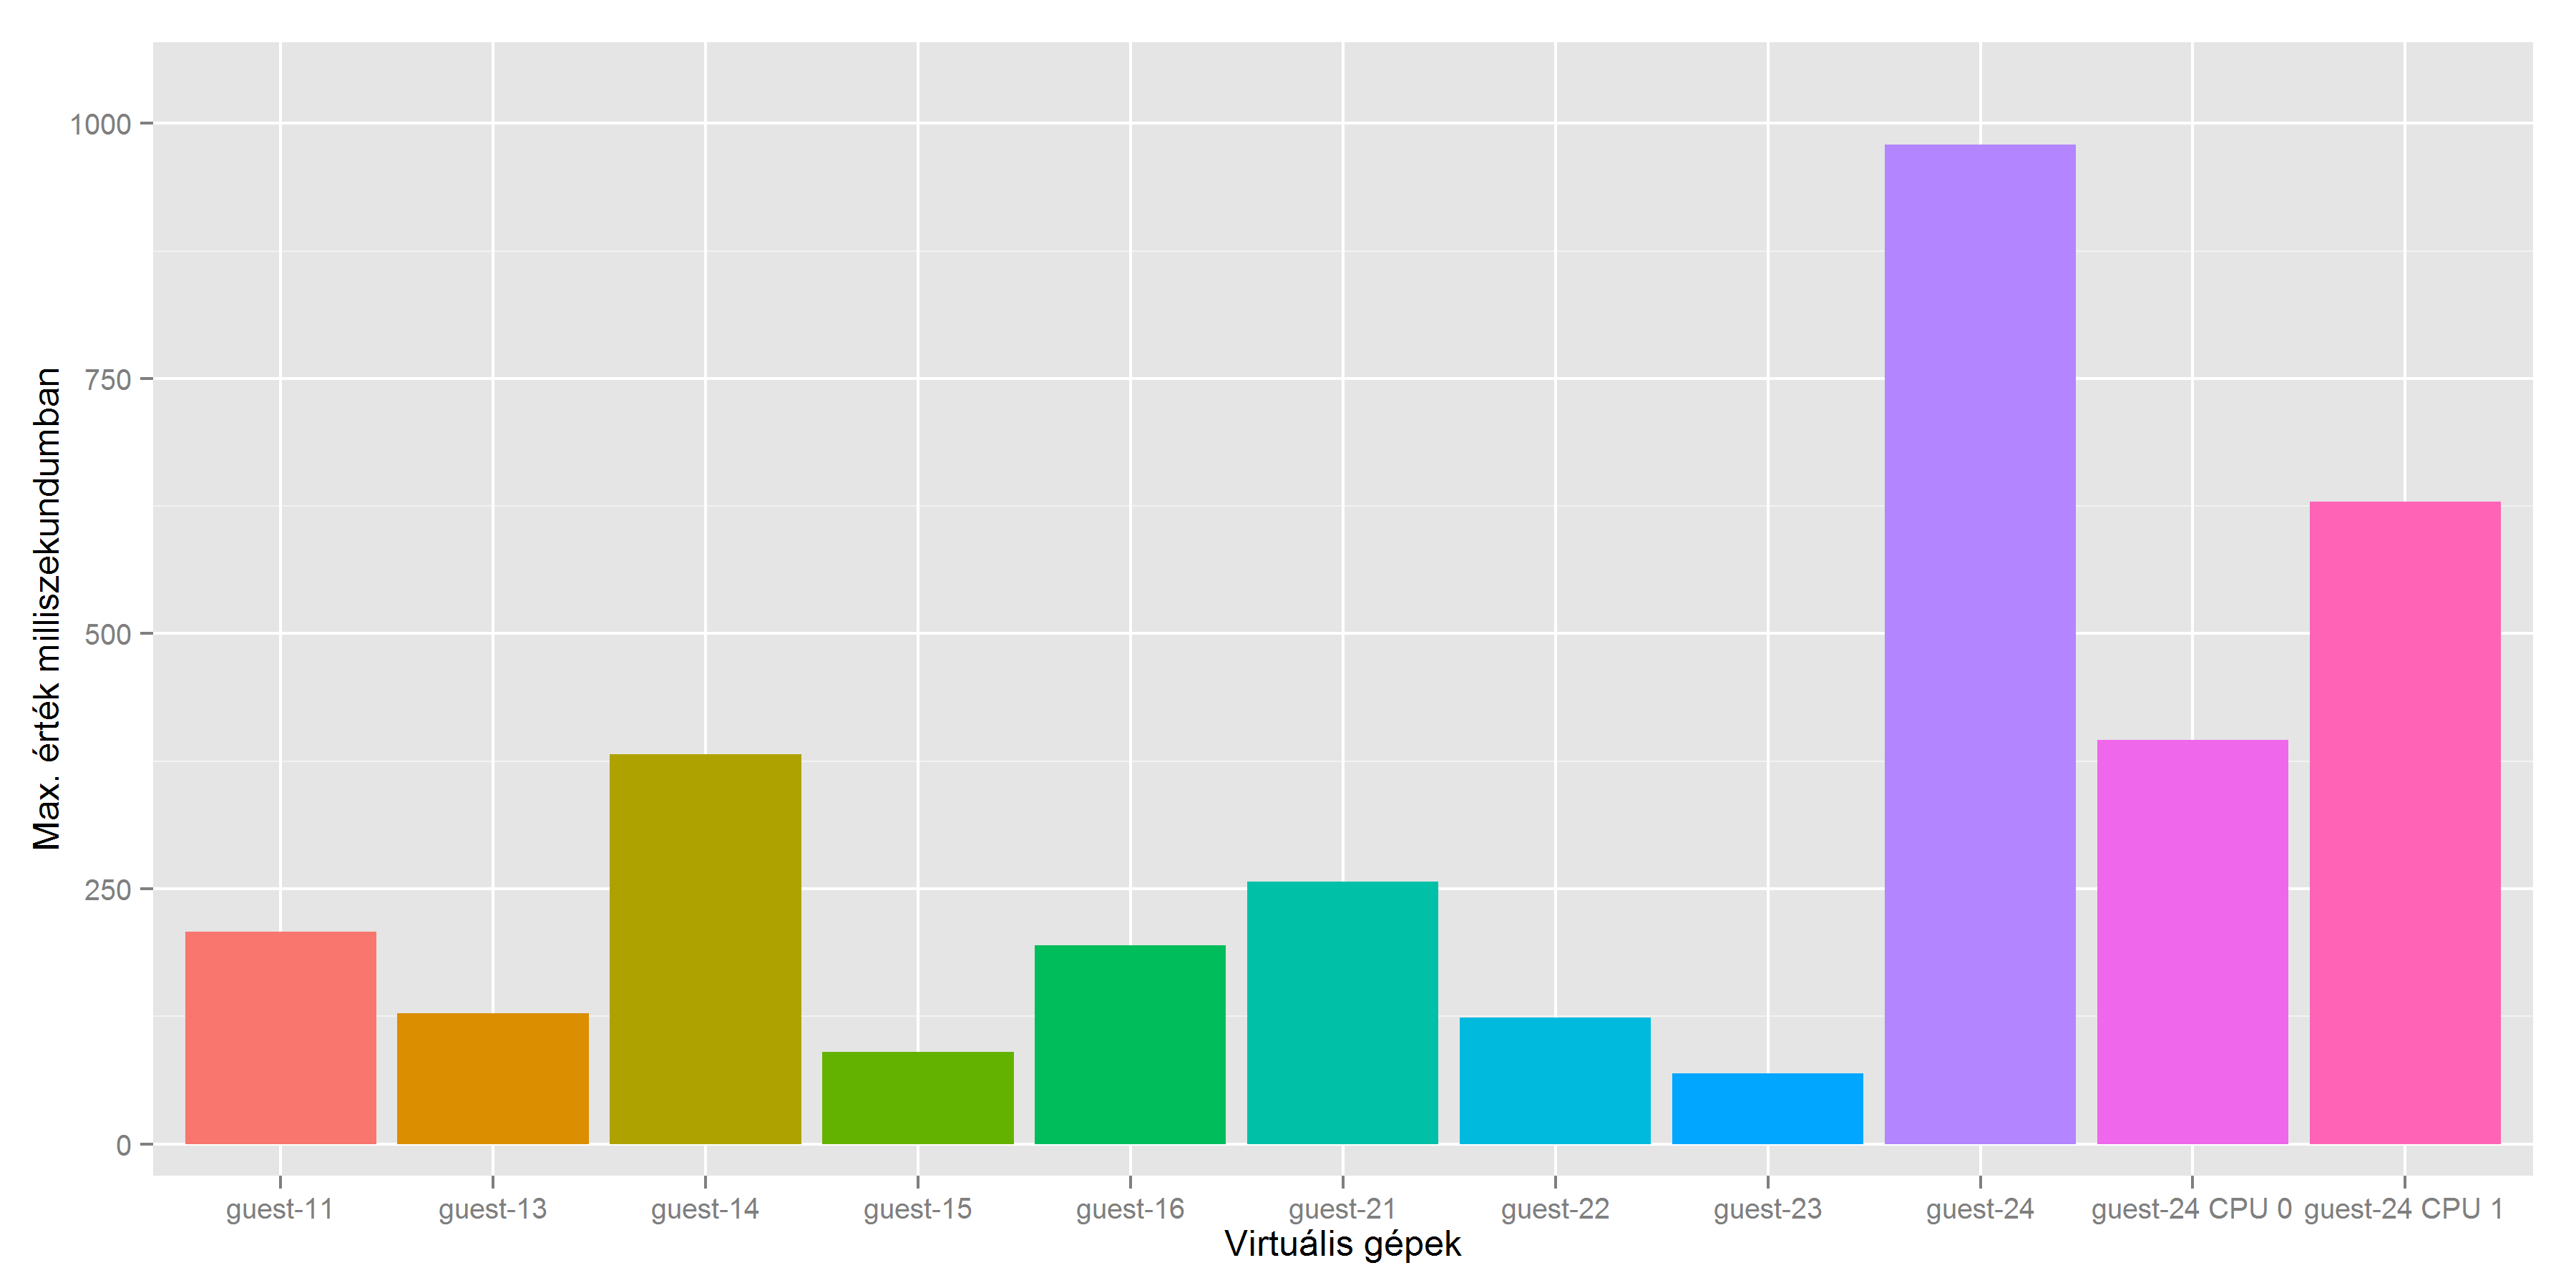
\includegraphics[width=0.80\textwidth]{figures/cpu_ready_summation-max-barchart.png}
\caption{A cpu.ready.summation maximális értéke az egyes VM-ek esetén \label{fig:cpu_ready_summation_max_barchart}}
\end{figure}

Amennyiben arra vagyunk kíváncsiak, hogy a rendszerünk mennyire üzemel a ready idők szempontjából a kritikus határokon belül, úgy azt \aref{fig:cpu_ready_summation_histograms}.~ábrákon (\aref{fig:cpu_ready_summation_histogram_wb}.~ábra esetében az 5 és kritikus 10\%-os határ is jelölve van) nézhetjük meg. Megállapítható, hogy még a legnagyobb érték sem éri az időablak 2.5\%-át sem, tehát a vizsgált infrastruktúrán esetében nincs CPU teljesítményből eredő probléma.

\begin{figure}[h!]
  \centering
  \subfloat[A VM-ek cpu.ready.summation eloszlása]{\label{fig:cpu_ready_summation_histogram}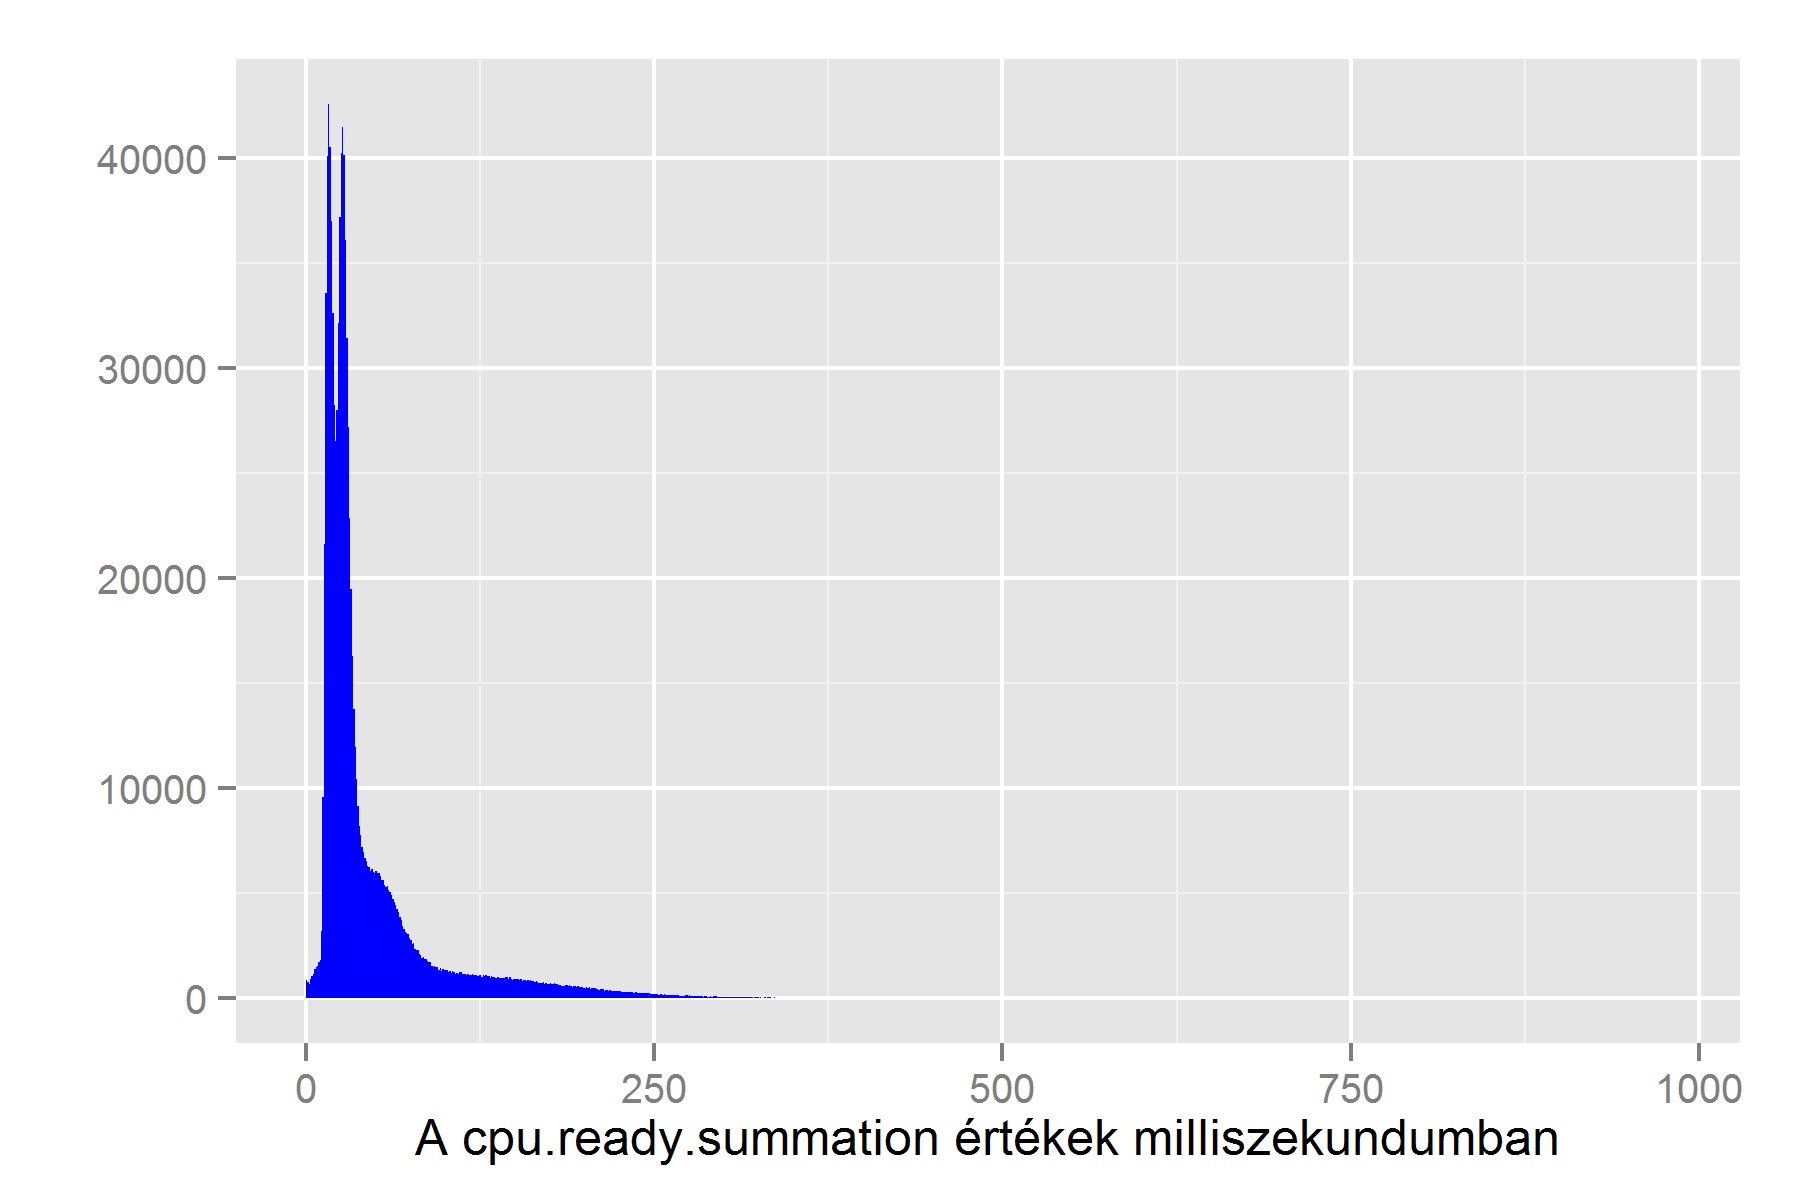
\includegraphics[width=0.45\textwidth]{figures/cpu_ready_summation-histogram.png}}                
  \subfloat[A VM-ek cpu.ready.summation eloszlása, az 5 és 10\%-os határokkal]{\label{fig:cpu_ready_summation_histogram_wb}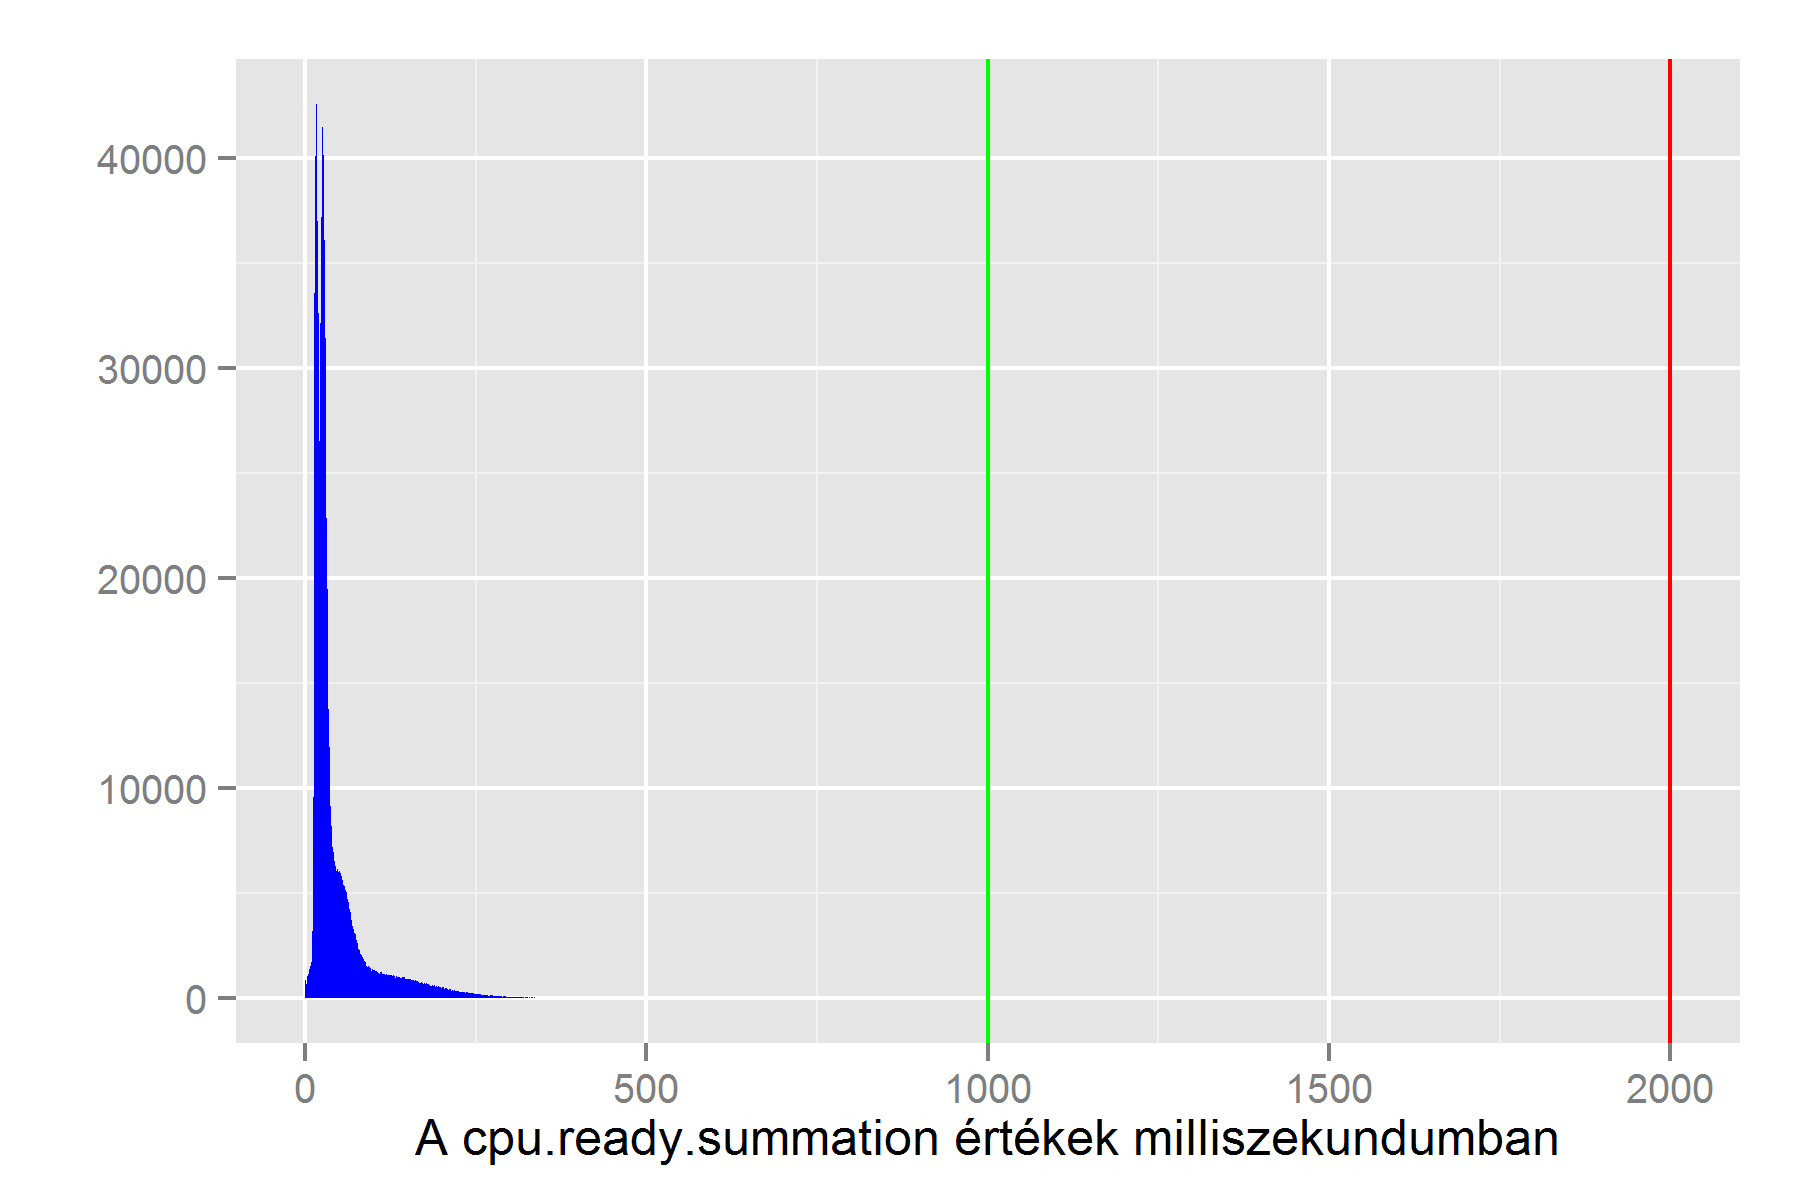
\includegraphics[width=0.45\textwidth]{figures/cpu_ready_summation-histogram-w-b.png}}
  \caption{A VM-ek cpu.ready.summation eloszlása}
  \label{fig:cpu_ready_summation_histograms}
\end{figure}
%#
%###############################################################################

\subsection{Összefüggés a wait, ready, run metrikák között}

A következőekben a wait, ready és run metrikák közötti összefüggést fogjuk megvizsgálni. Tudjuk, hogy a három metrika összege kiadja a mérési ablak nagyságát, tehát a CPU 20 másodpercből $X$ időt futási, $Y$ időt várakozási és $Z$ időt futásra kész állapotban tölt, amelyekre $X+Y+Z=20000$. \Aref{fig:cpu_run_wait_ready-guest-15-01}.~ábrán a \textit{guest-15} azonosítójú virtuális gép ezen metrikáinak alakulása látható a teljes mérési időszakban.

\begin{figure}[h!]
\centering
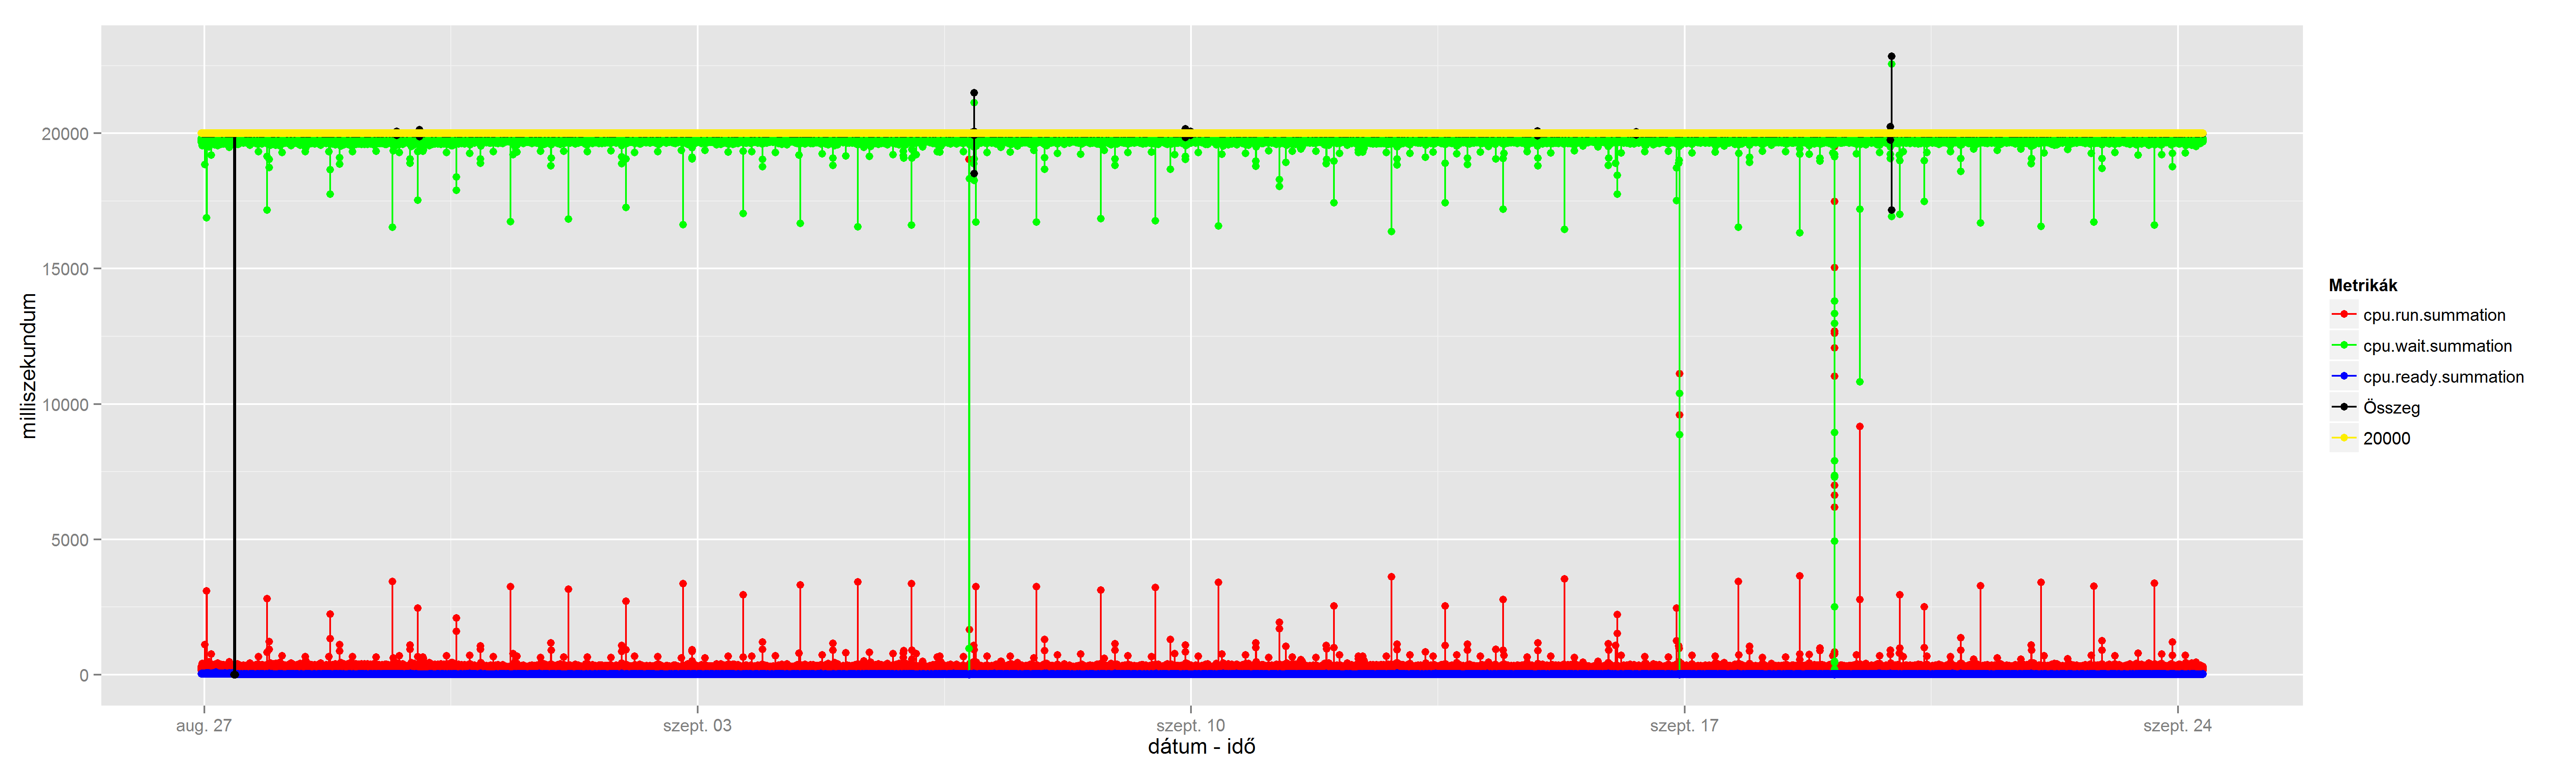
\includegraphics[width=1.00\textwidth]{figures/cpu_run_wait_ready-guest-15-20120826230140-20120924083120.png}
\caption{ A guest-15 VM CPU állapotainak alakulása a teljes megfigyelési időintervallumban \label{fig:cpu_run_wait_ready-guest-15-01}}
\end{figure}

Megfigyelhető, hogy a három érték összege több helyen is eltér a várt 20000-es értéktől. Ha szűkebb időintervallumban vizsgáljuk az adatok alakulását (\ref{fig:cpu_run_wait_ready-guest-15-02}.~ábra) megállapíthatjuk, hogy a \texttt{cpu.wait.summation} hibás értékeiből származnak az eltérések. Ezek értékeit \aref{fig:cpu_run_wait_ready-diff-guest-15}.~ábrán láthatjuk. 


\begin{figure}[h!]
\centering
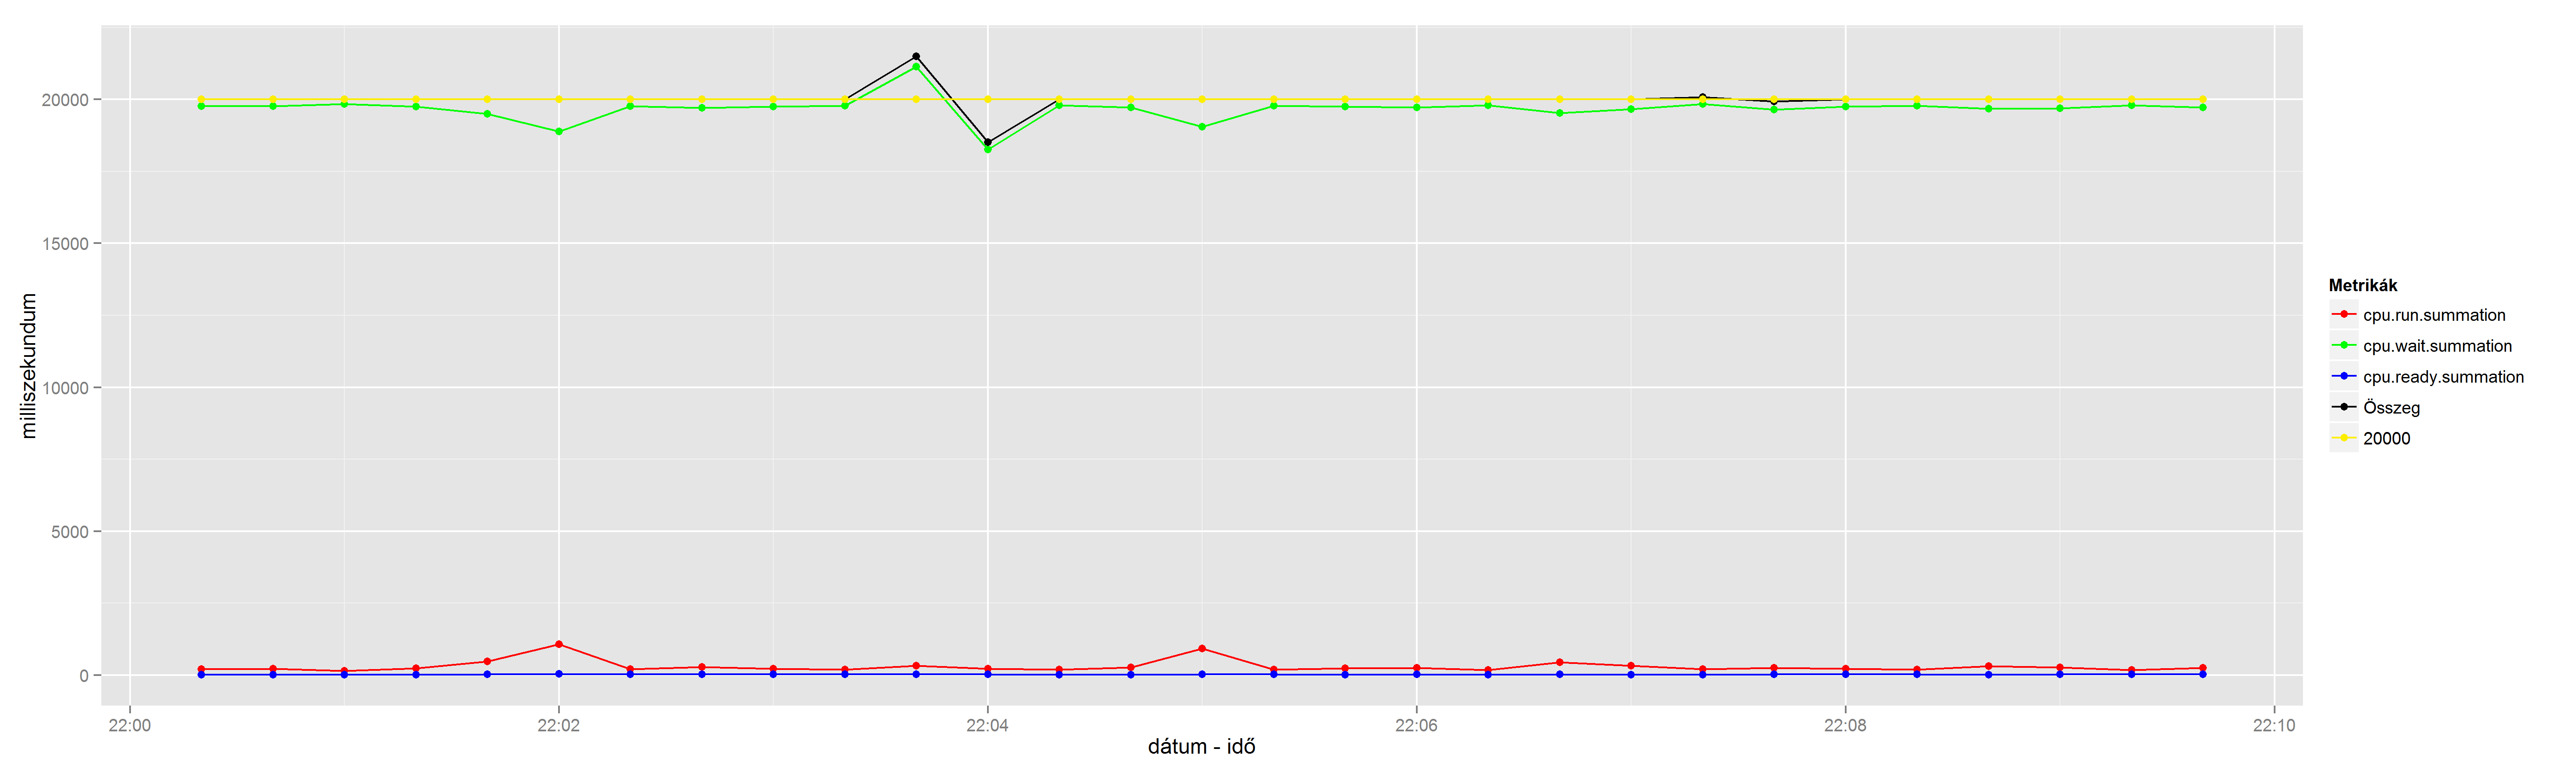
\includegraphics[width=1.00\textwidth]{figures/cpu_run_wait_ready-guest-15-20120906220000-20120906221000.png}
\caption{ A guest-15 VM CPU állapotainak alakulása 2012.09.06. 22:00:00 és 2012.09.06. 22:10:00 között \label{fig:cpu_run_wait_ready-guest-15-02}}
\end{figure}

\begin{figure}[h!]
\centering
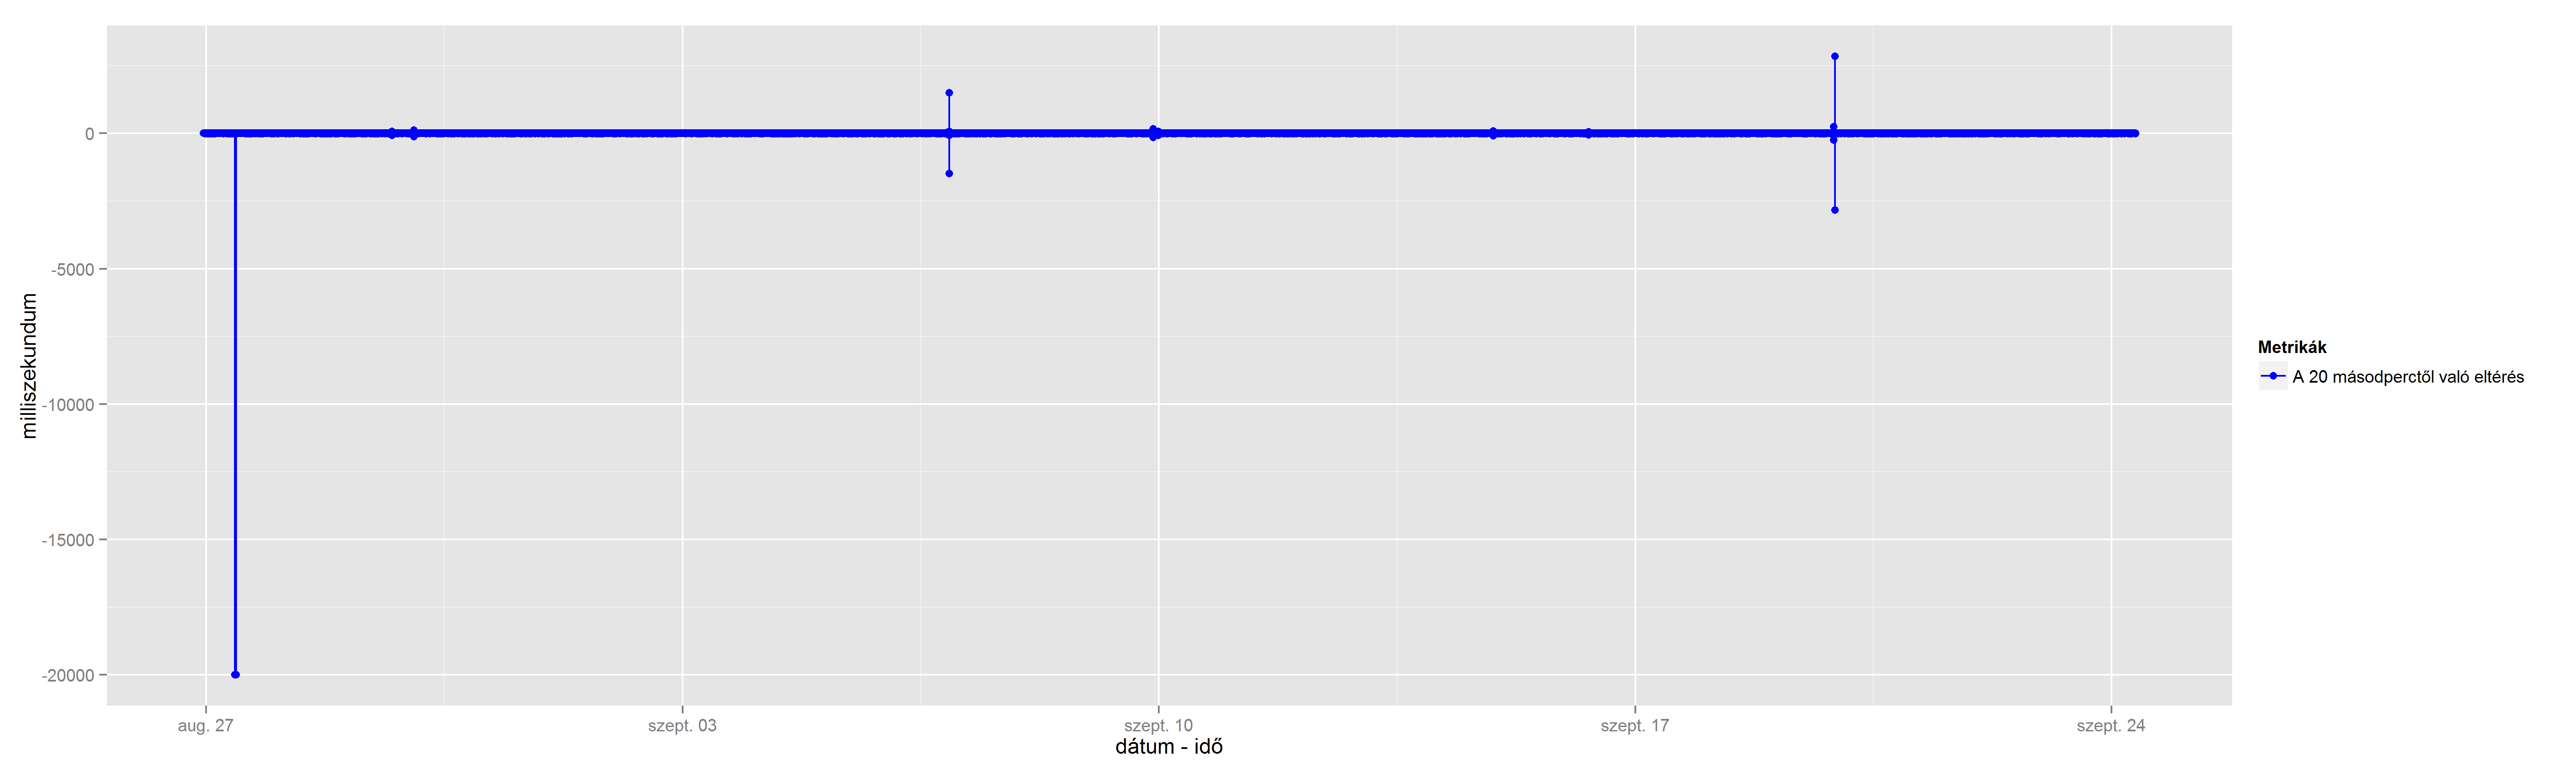
\includegraphics[width=1.00\textwidth]{figures/cpu_run_wait_ready-diff-guest-15-20120826230140-20120924083120.png}
\caption{ A guest-15 VM run, wait és ready összegek eltérései a 20 másodperchez képest \label{fig:cpu_run_wait_ready-diff-guest-15}}
\end{figure}

A guest-15 kiugró értékeitől kisebb eltéréseket is megfigyelhetünk más virtuális gépeknél. \Aref{fig:cpu_run_wait_ready-diff-guest-13}.~ábrán a \textit{guest-13} méréseinek számított értéke látható. Itt max. 6 milliszekundumos különbségeket találunk.

\begin{figure}[h!]
\centering
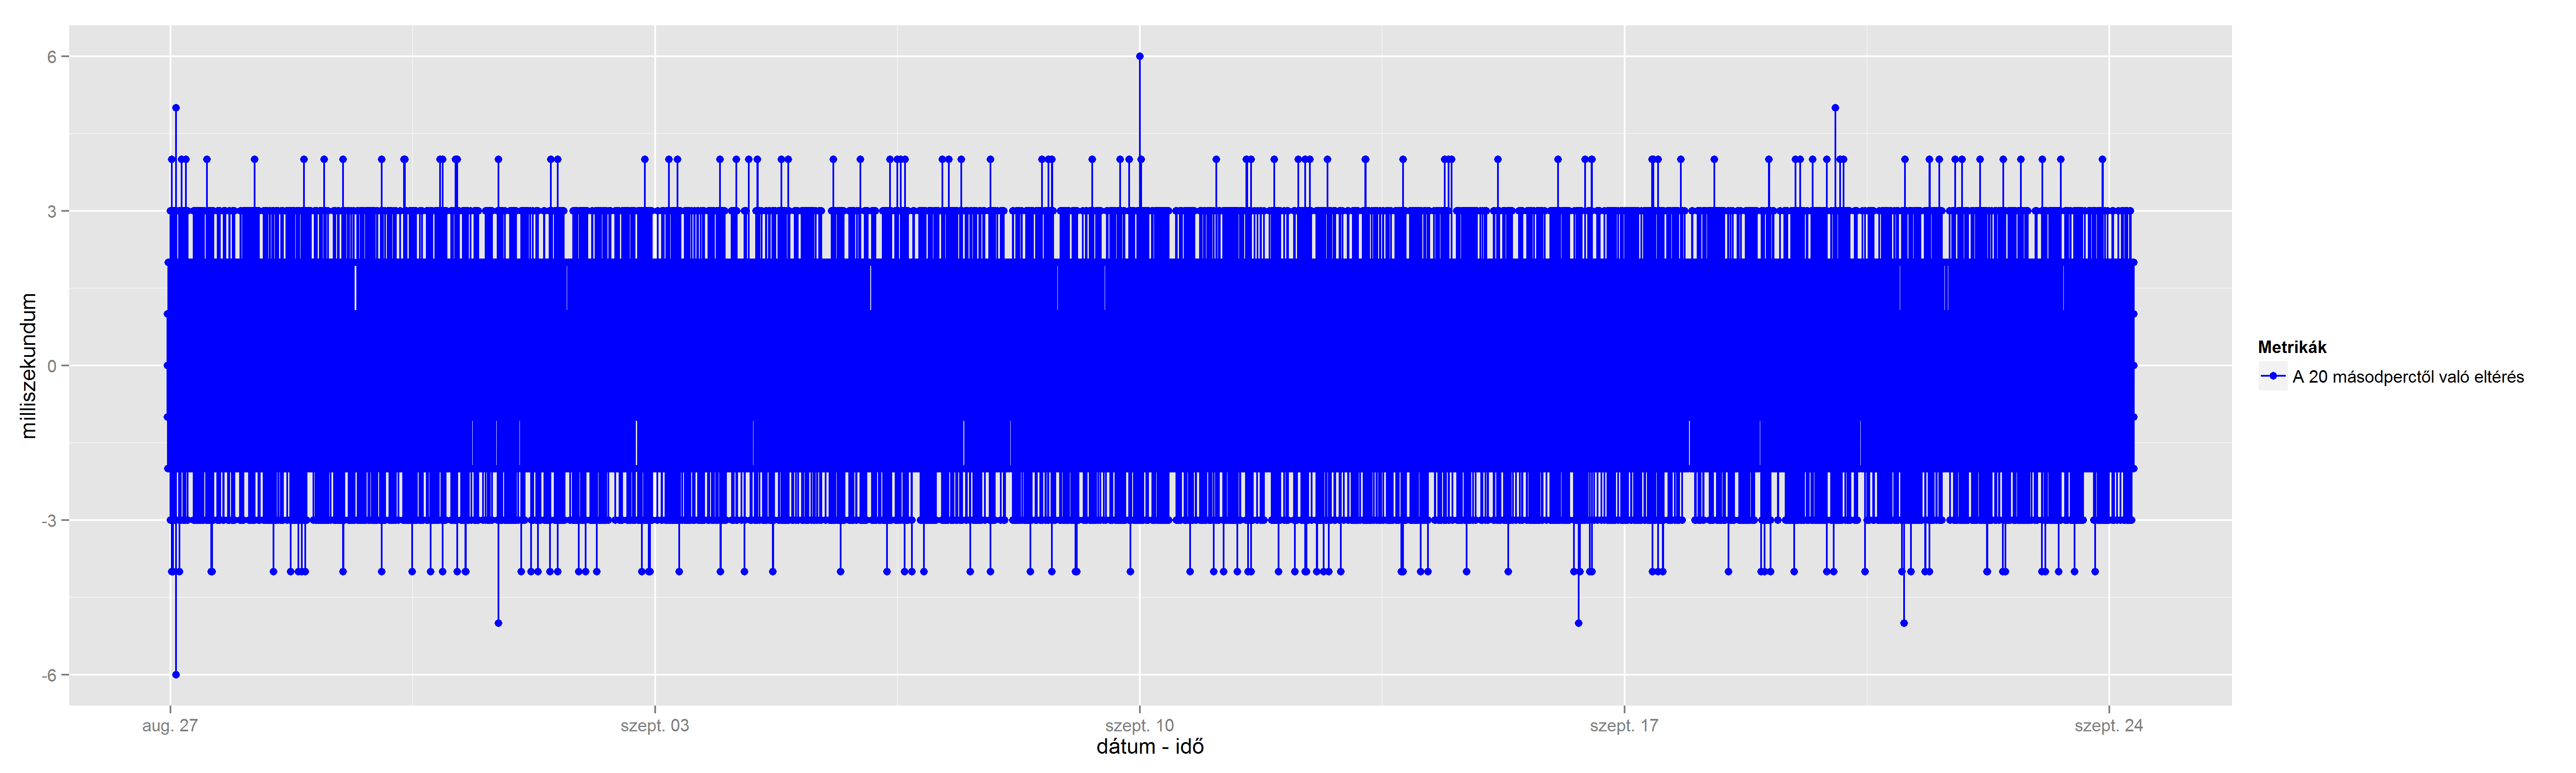
\includegraphics[width=1.00\textwidth]{figures/cpu_run_wait_ready-diff-guest-13-20120826230140-20120924083120.png}
\caption{ A guest-13 VM run, wait és ready összegek eltérései a 20 másodperchez képest \label{fig:cpu_run_wait_ready-diff-guest-13}}
\end{figure}

\Aref{fig:cpu_run_wait_ready-diff-dist}.~ábrán az eltérések eloszlását láthatjuk a teljes rendszerre nézve. Megállapítható, hogy az eltérések többsége 6 milliszekundumon belüli értéket vesz fel. Ha ugyanezt az eloszlást logaritmikus skálán nézzük, akkor viszont az is kiderül, hogy milyen eltérések vannak a teljes mért időszakban (\ref{fig:cpu_run_wait_ready-diff-dist-log}).

\begin{figure}[h!]
\centering
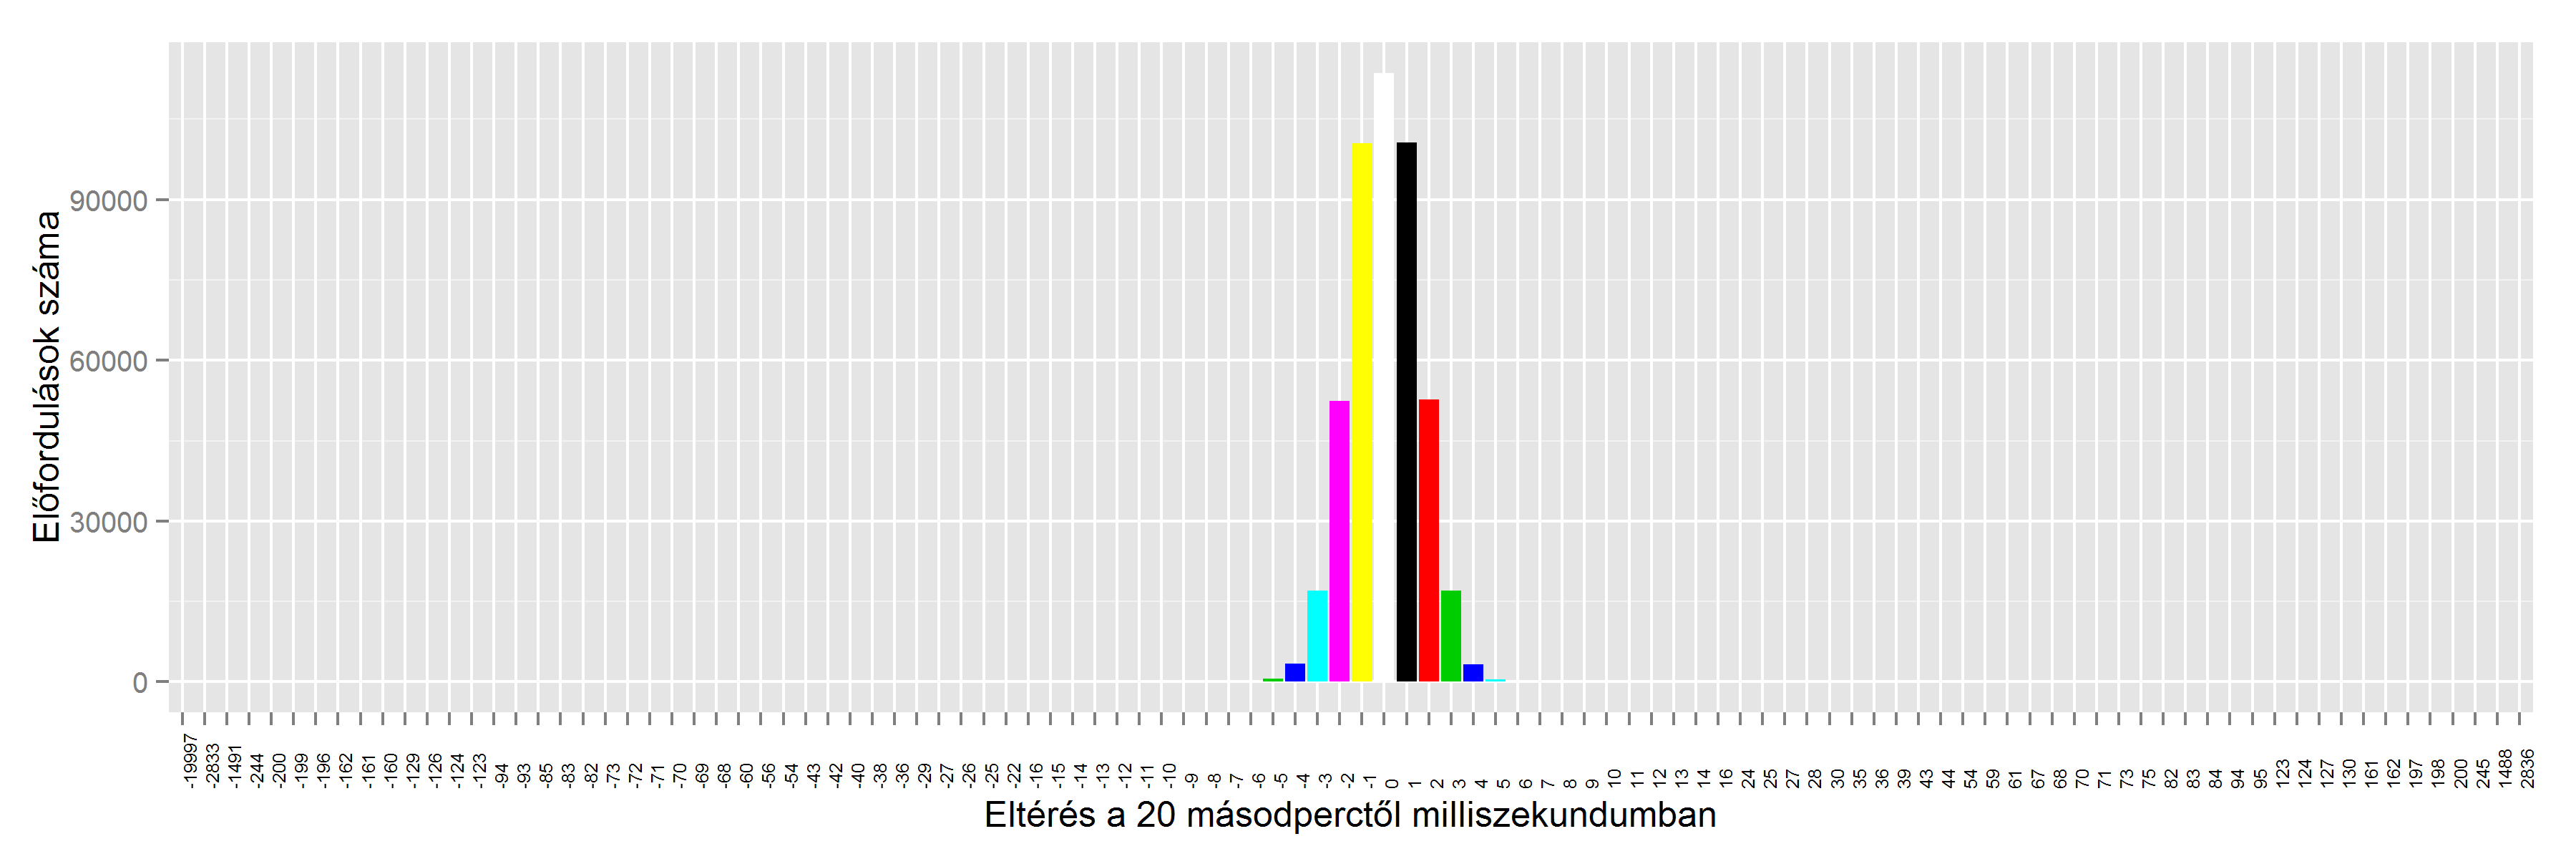
\includegraphics[width=1.00\textwidth]{figures/cpu_run_wait_ready-diff-dist-20120826230140-20120924083120.png}
\caption{ Előforduló eltérések a 20000 milliszekundumhoz képest \label{fig:cpu_run_wait_ready-diff-dist}}
\end{figure}

\begin{figure}[h!]
\centering
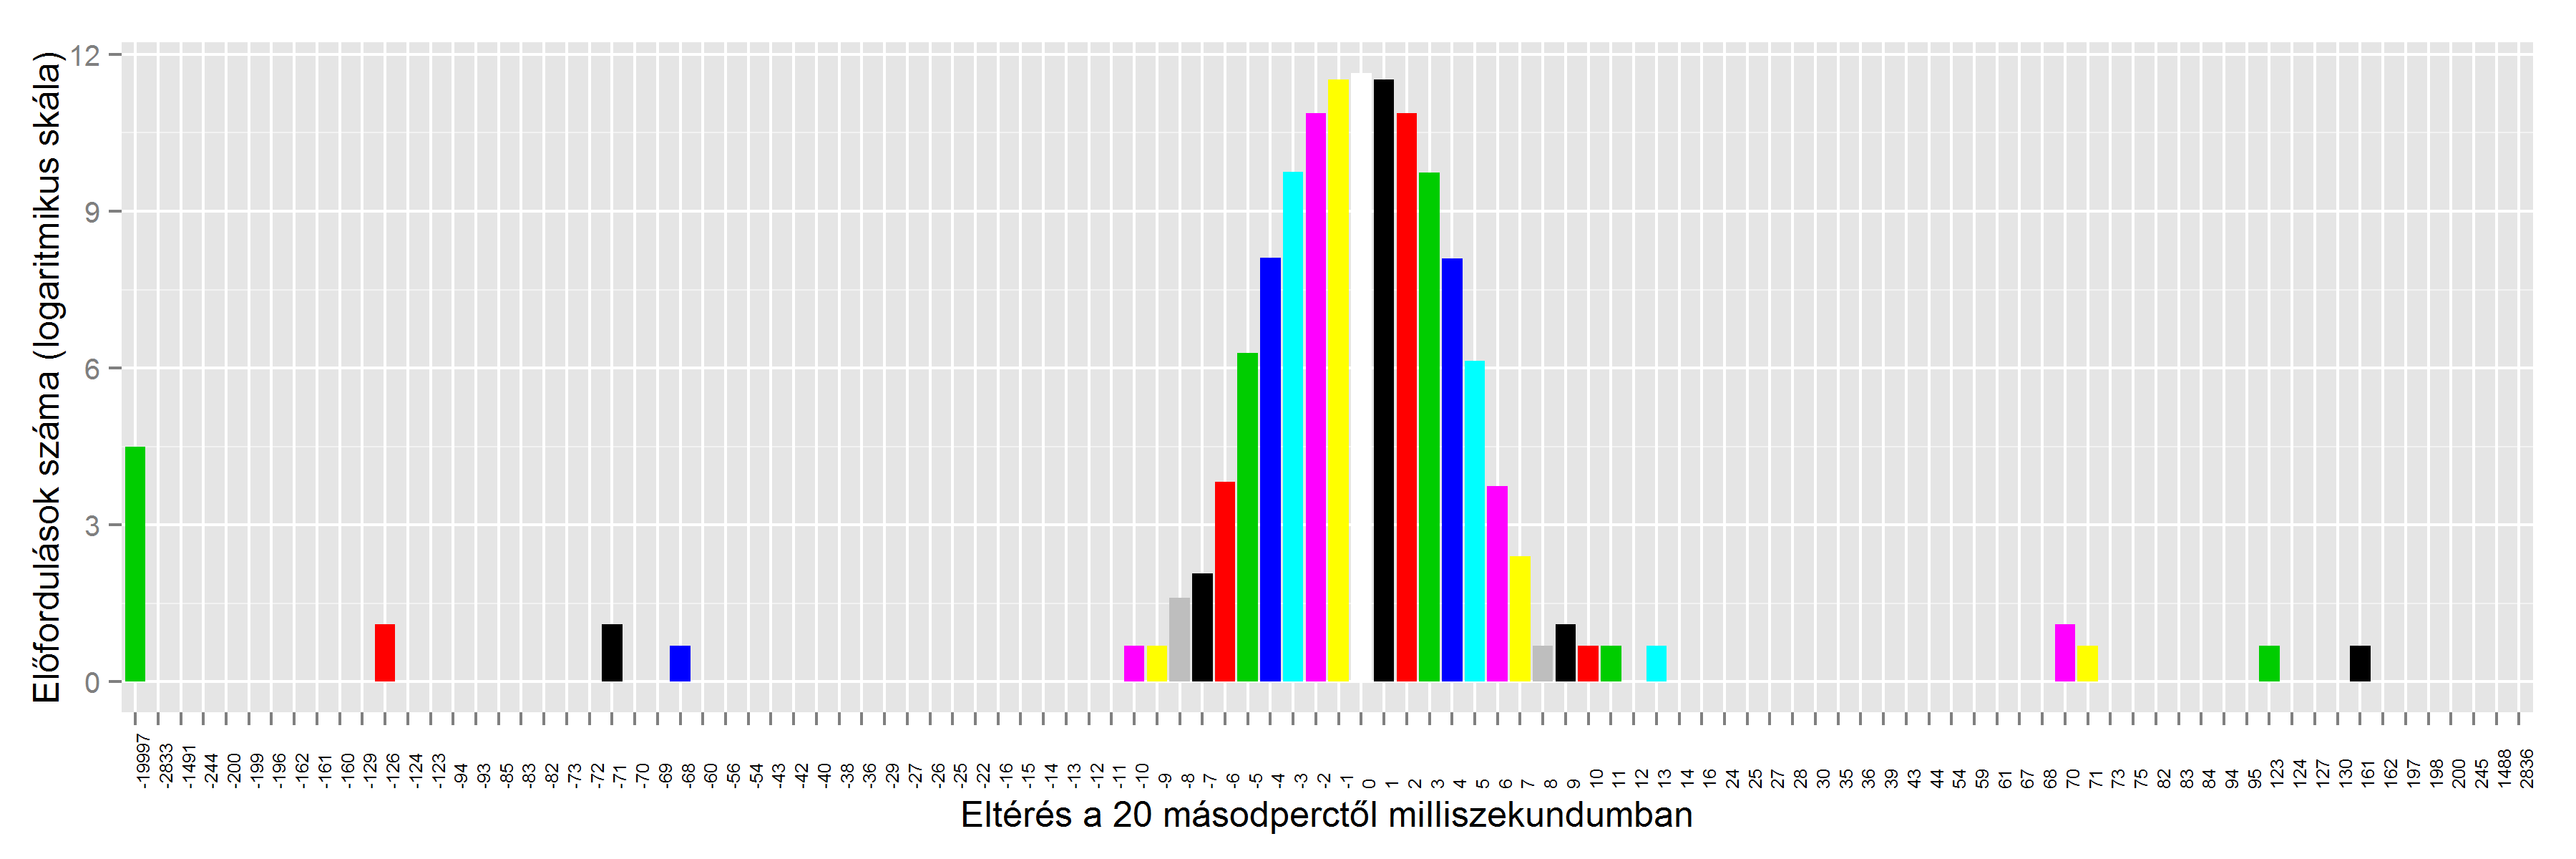
\includegraphics[width=1.00\textwidth]{figures/cpu_run_wait_ready-diff-dist-log-20120826230140-20120924083120.png}
\caption{ Előforduló eltérések a 20000 milliszekundumhoz képest (logaritmikus skálán)\label{fig:cpu_run_wait_ready-diff-dist-log}}
\end{figure}

A vizsgálatból megállítható, hogy bár a három metrika összege megközelítve kiadja a mérési időablak nagyságának értékét, de nincs teljesen megbízható lehetőség arra, hogy esetlegesen valamelyik metrika eltárolása helyett azt a másik kettő alapján számoljuk ki.

%\subsection{Összefüggés az idle, swapwait, system metrikák között}
%
%\todo{Megcsinálni!}
%
%\begin{table}[h]
%	\caption{A cpu.system.summation metrika}
%	\centering
%	\small
%	\begin{tabular}{| p{3.5cm} | p{7.5cm} | p{2cm} |}
%		\hline
%		\rowcolor{tc_bone} \textbf{Metrika} & \textbf{Leírás} & \textbf{Mértékegység} \\
%		\hline
%		cpu.system.summation & Azoknak az időknek az összege, amelyet a virtuális CPU a virtuális gépben rendszer folyamatok (megszakítás, I/O) kezelésével tölt. Ez nem a vendég operációs rendszer, hanem a kiszolgáló által látott érték. & milliszekundum \\ 
%		\hline
%	\end{tabular}
%	\normalsize
%	\label{tab:cpu.system.summation}
%\end{table}


\subsection{Korreláció vizsgálata a cpu.usage.average és cpu.usagemhz.average metrikák között}



Vizsgáljuk meg a \texttt{cpu.usage.average} és \texttt{cpu.usagemhz.average} metrikák közötti korrelációt. A korreláció nagyságát vizuálisan \aref{fig:corrgram-hosts}.~ábra mutatja.

Megállapítható, hogy a két metrika közötti összefüggés miatt az egyikük akár el is hagyható a monitorozás/naplózás során, hiszen nem nyújt új információt az infrastruktúráról. 

\begin{figure}[h!]
  \centering
  \subfloat[host-01 (Korreláció: $0,999999734514543$)]{\label{fig:corrgram-host-01}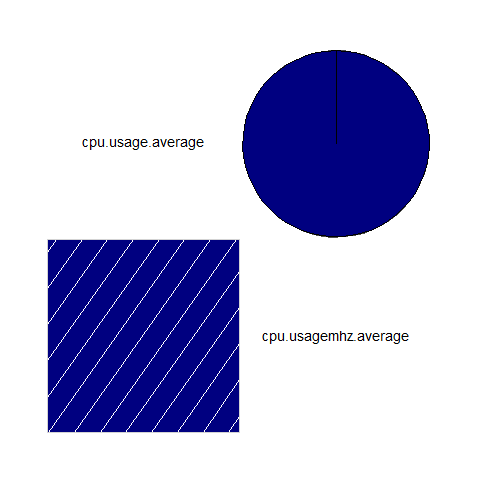
\includegraphics[width=0.45\textwidth]{figures/corrgram-host-01-0999999734514543.png}}                
  \subfloat[host-02 (Korreláció: $0,999999692814215$)]{\label{fig:corrgram-host-01}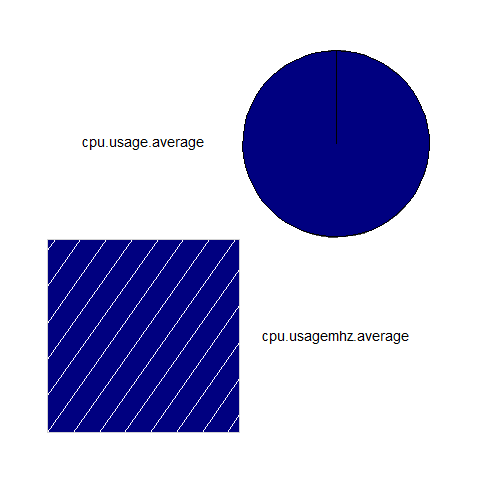
\includegraphics[width=0.45\textwidth]{figures/corrgram-host-02-0999999692814215.png}}
  \caption{A cpu.usage.average és cpu.usagemhz.average metrikák közötti korreláció}
  \label{fig:corrgram-hosts}
\end{figure}

\section{Lemez metrikák}

\todo{Írni a lemezmetrikákról általánosan!}

\todo{Forrás: \url{http://www.vmware.com/support/developer/vc-sdk/visdk400pubs/ReferenceGuide/disk_counters.html}}

\subsection{Összefüggés a disk.deviceLatency.average, disk.kernelLatency.average, \\ disk.totallatency.average metrikák között}

\todo{Megcsinálni!}



\begin{figure}[h!]
\centering
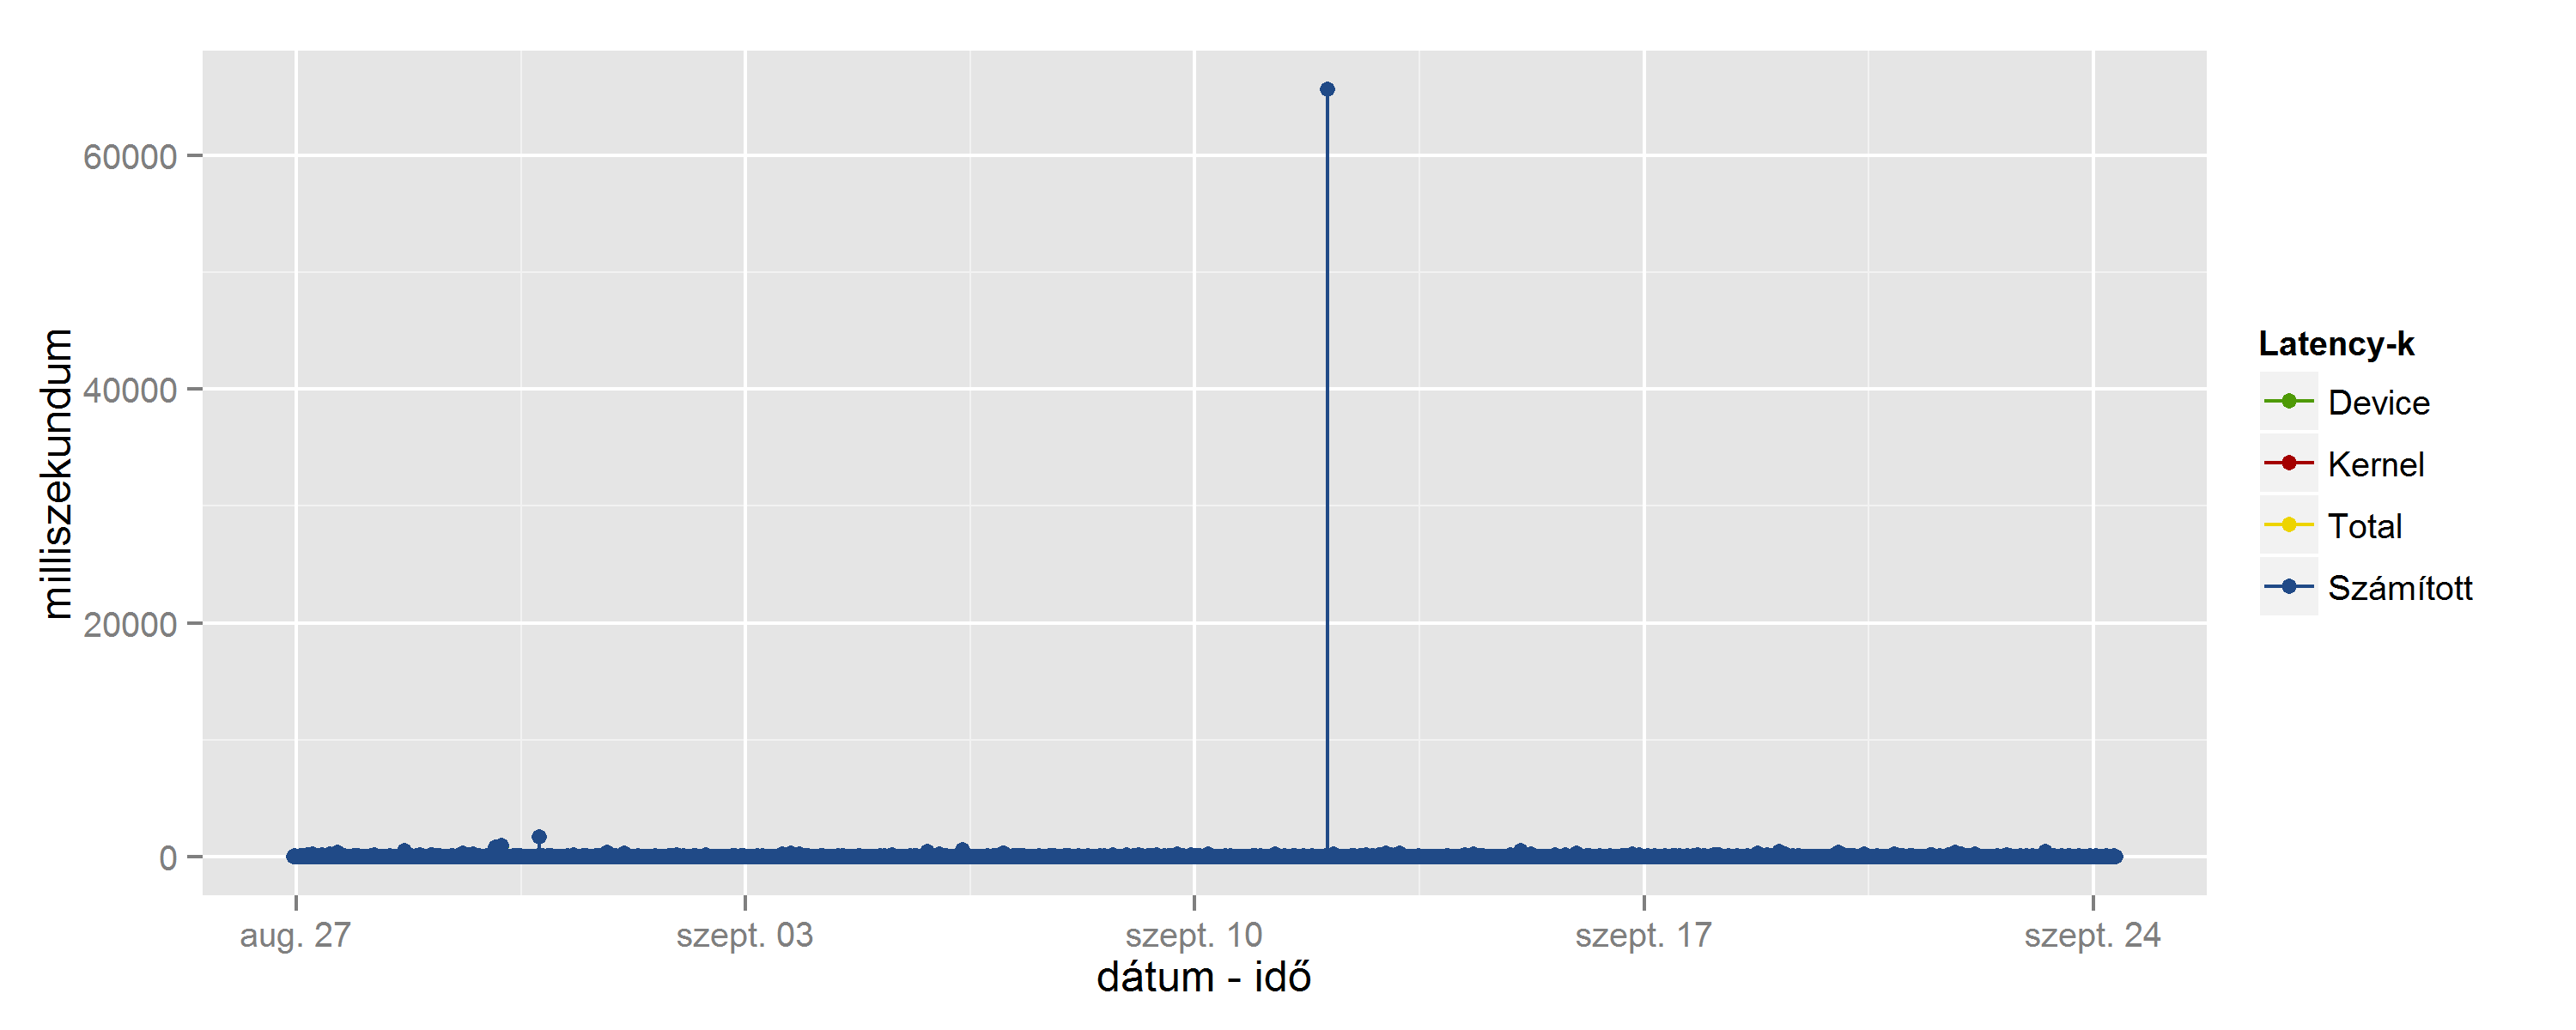
\includegraphics[width=1.00\textwidth]{figures/disk_metrics_sumlatency-20120826230140-20120924083120.png}
\caption{ Lemezkésleltetések a host-01 esetében a teljes mérési időintervallumon \label{fig:disk_metrics_sumlatency-01}}
\end{figure}

\begin{figure}[h!]
\centering
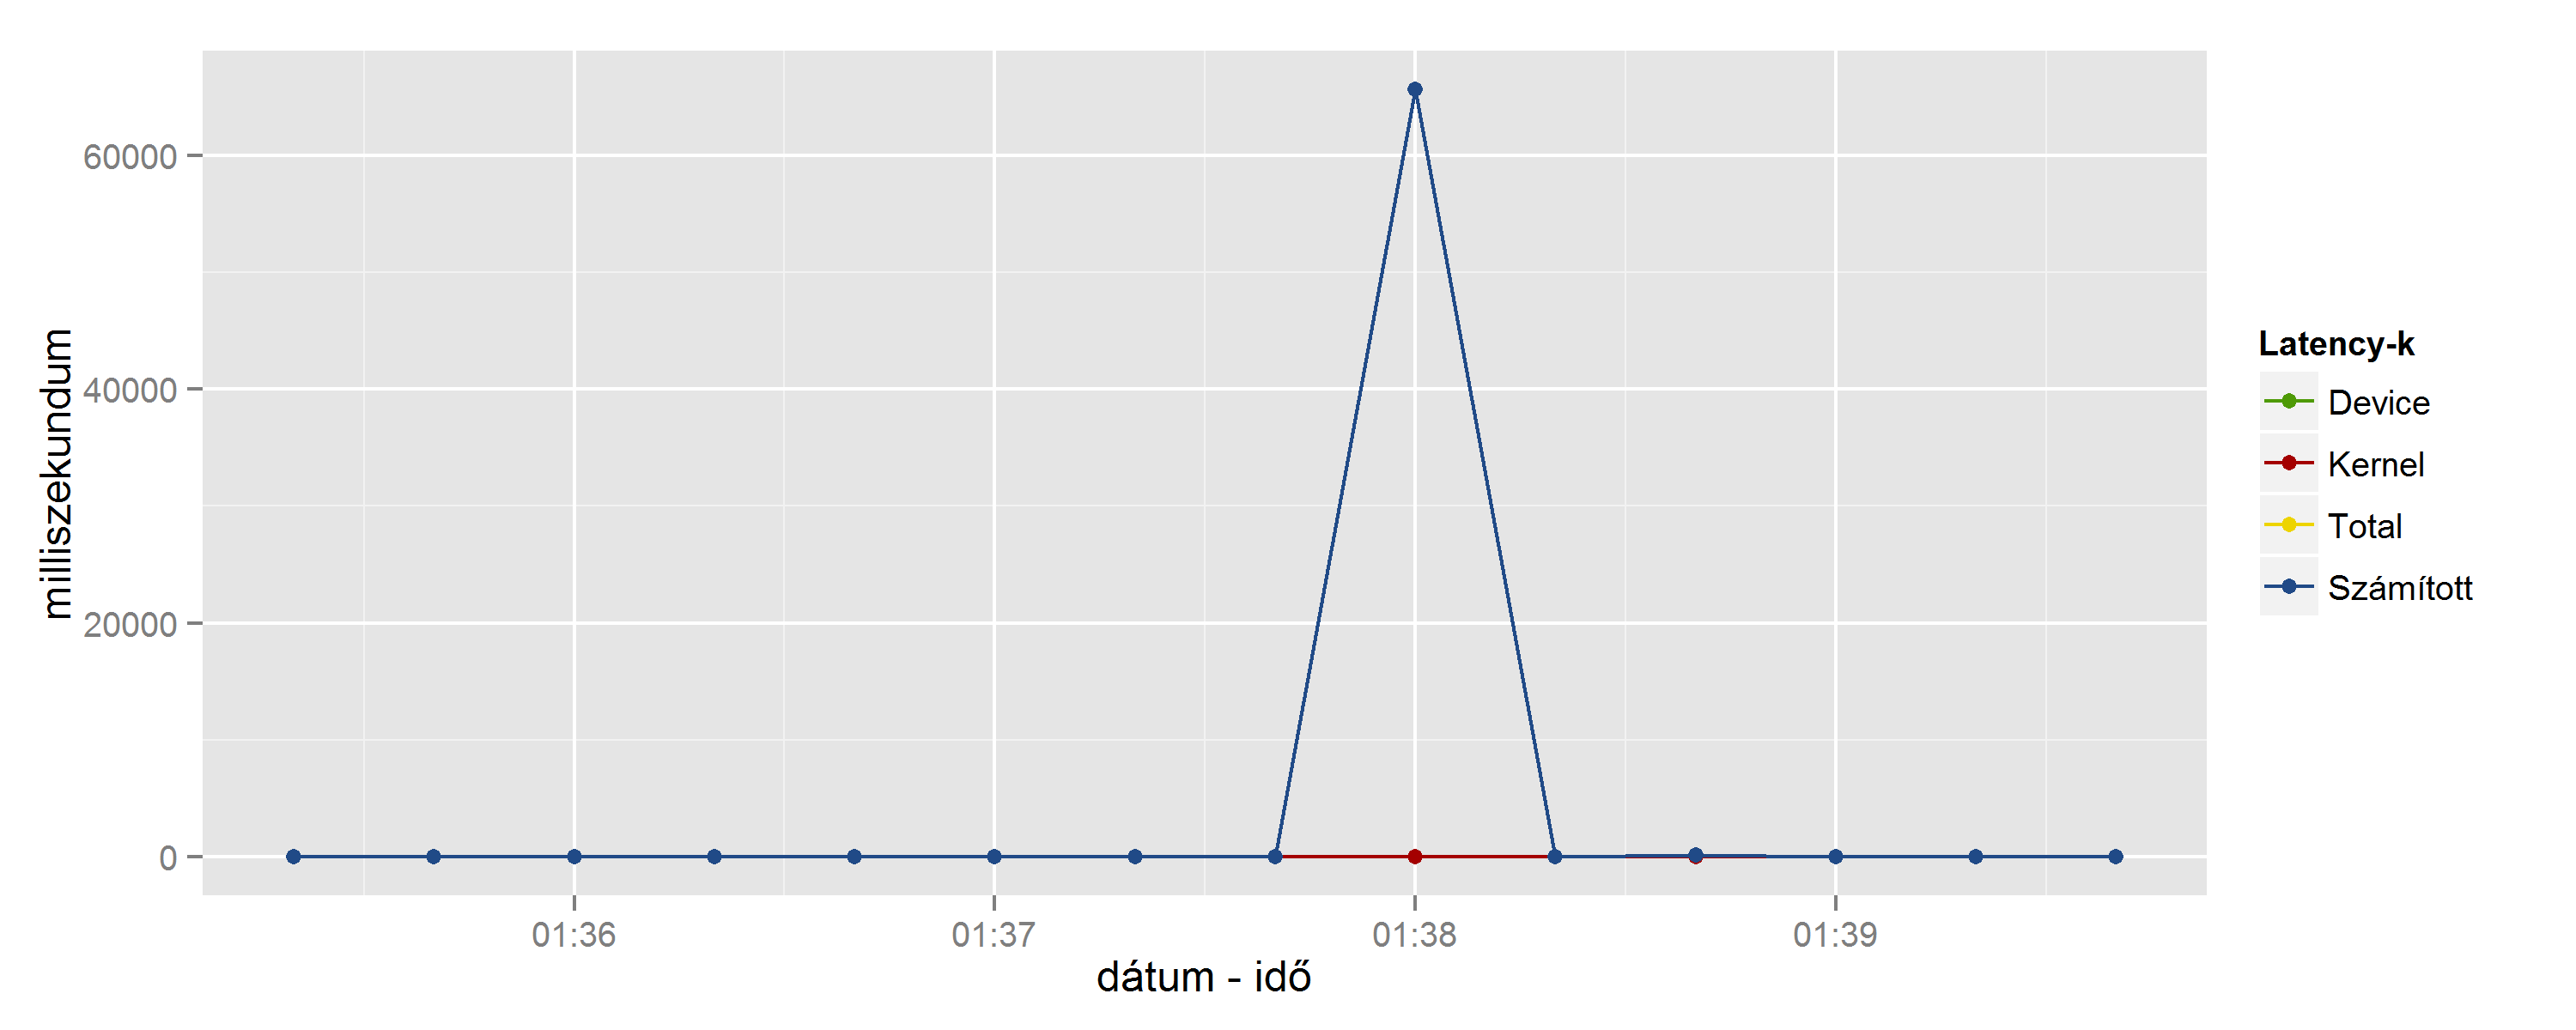
\includegraphics[width=1.00\textwidth]{figures/disk_metrics_sumlatency-20120912013500-20120912014000.png}
\caption{ Lemezkésleltetések a host-01 esetében 2012.09.12. 01:35:00 és 2012.09.12. 01:40:00 között \label{fig:disk_metrics_sumlatency-02}}
\end{figure}



\subsection{Összefüggés a storagepath, storageadapter, disk latency-k között}

\todo{Megcsinálni!}

\begin{figure}[h!]
\centering
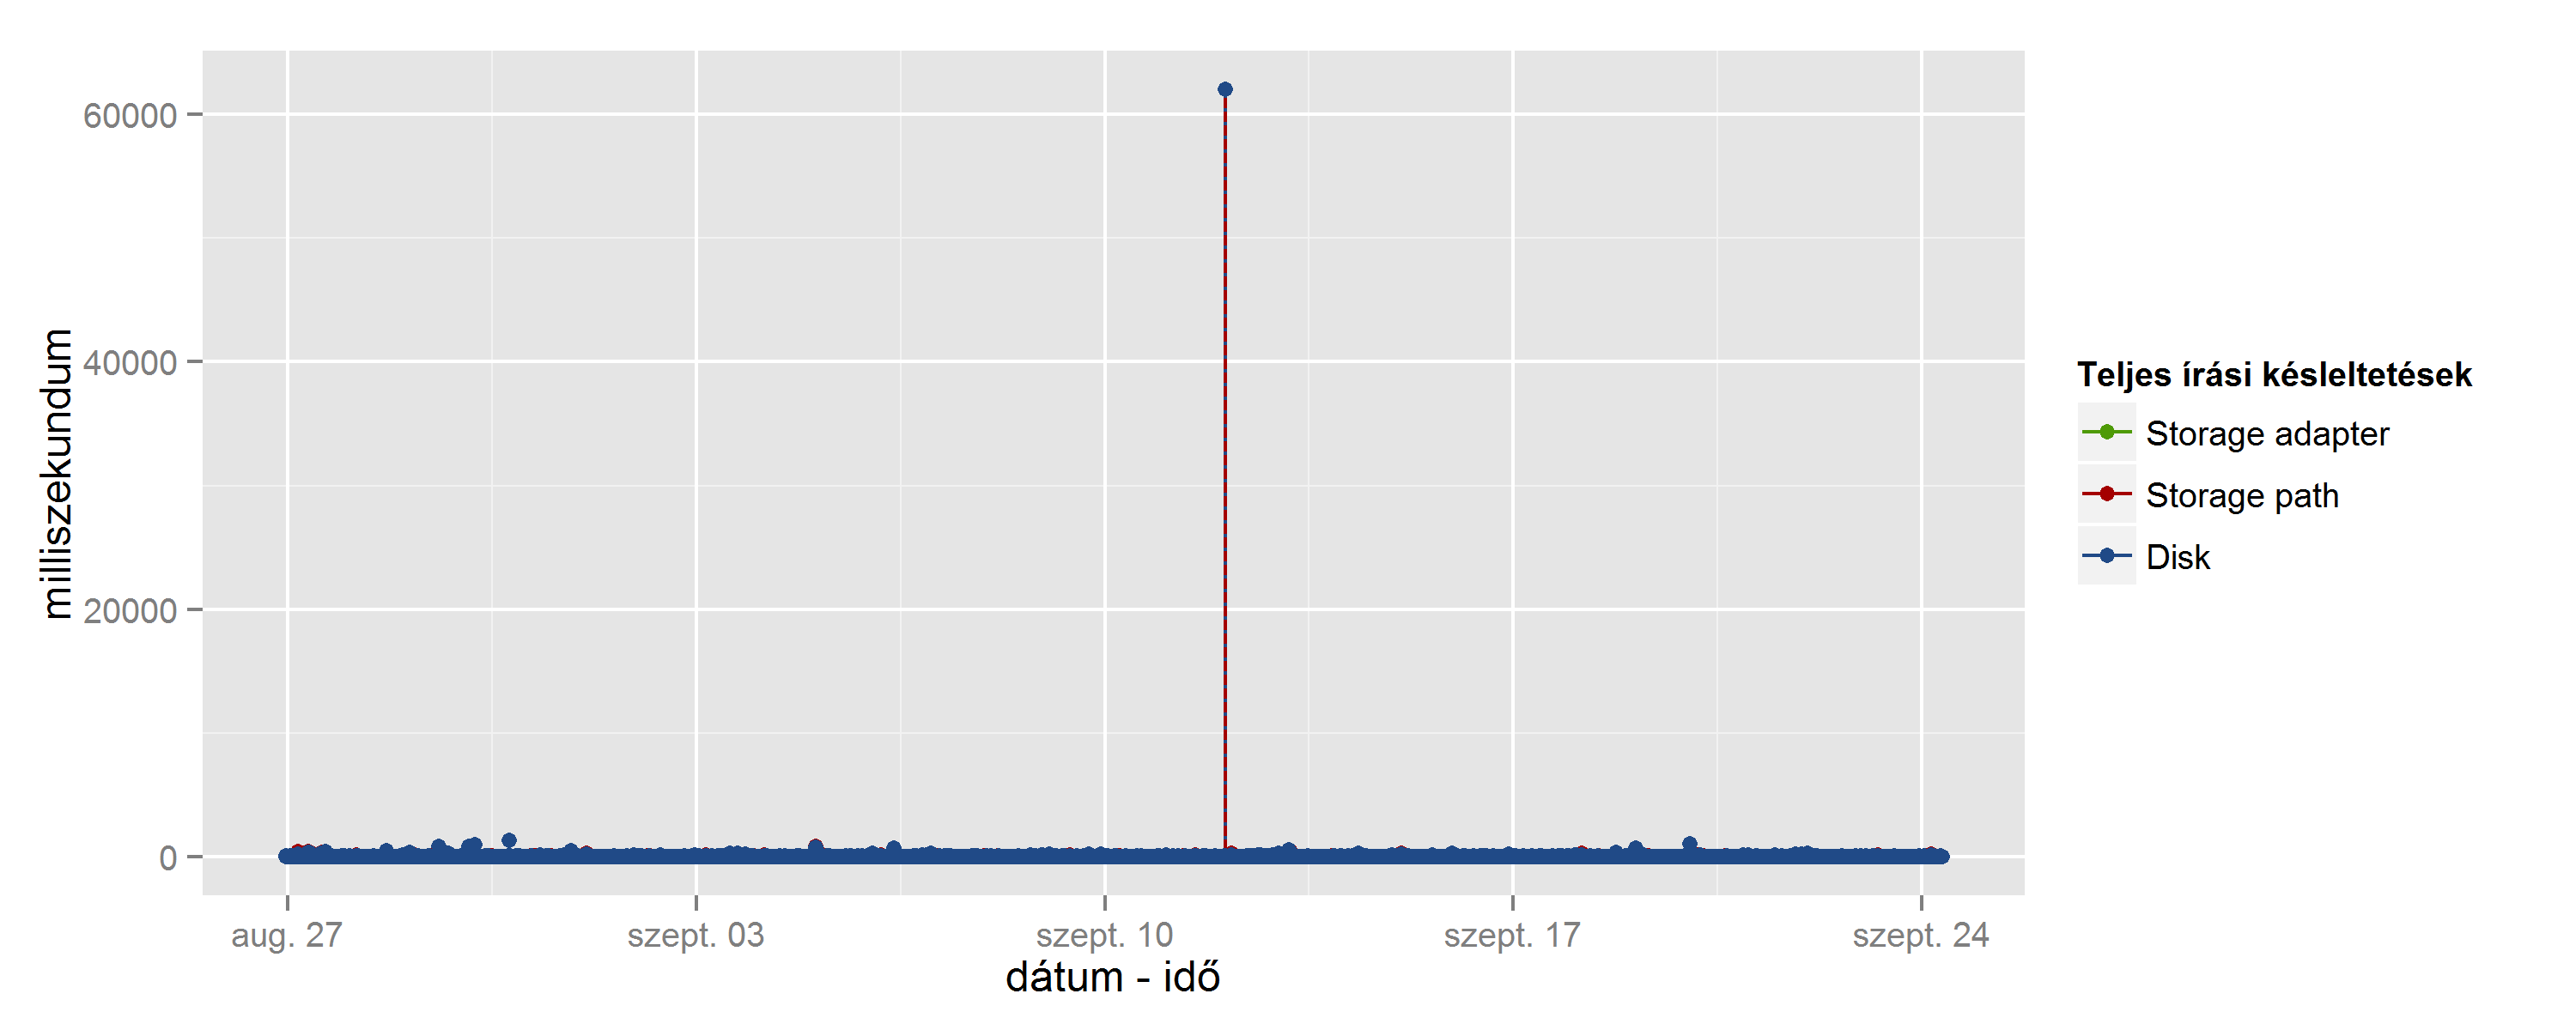
\includegraphics[width=1.00\textwidth]{figures/disk_metrics_storage_latency-20120826230140-20120924083120.png}
\caption{ Storage késleltetés a host-01 esetében a teljes megfigyelési időintervallumon \label{fig:disk_metrics_storage_latency-01}}
\end{figure}

\begin{figure}[h!]
\centering
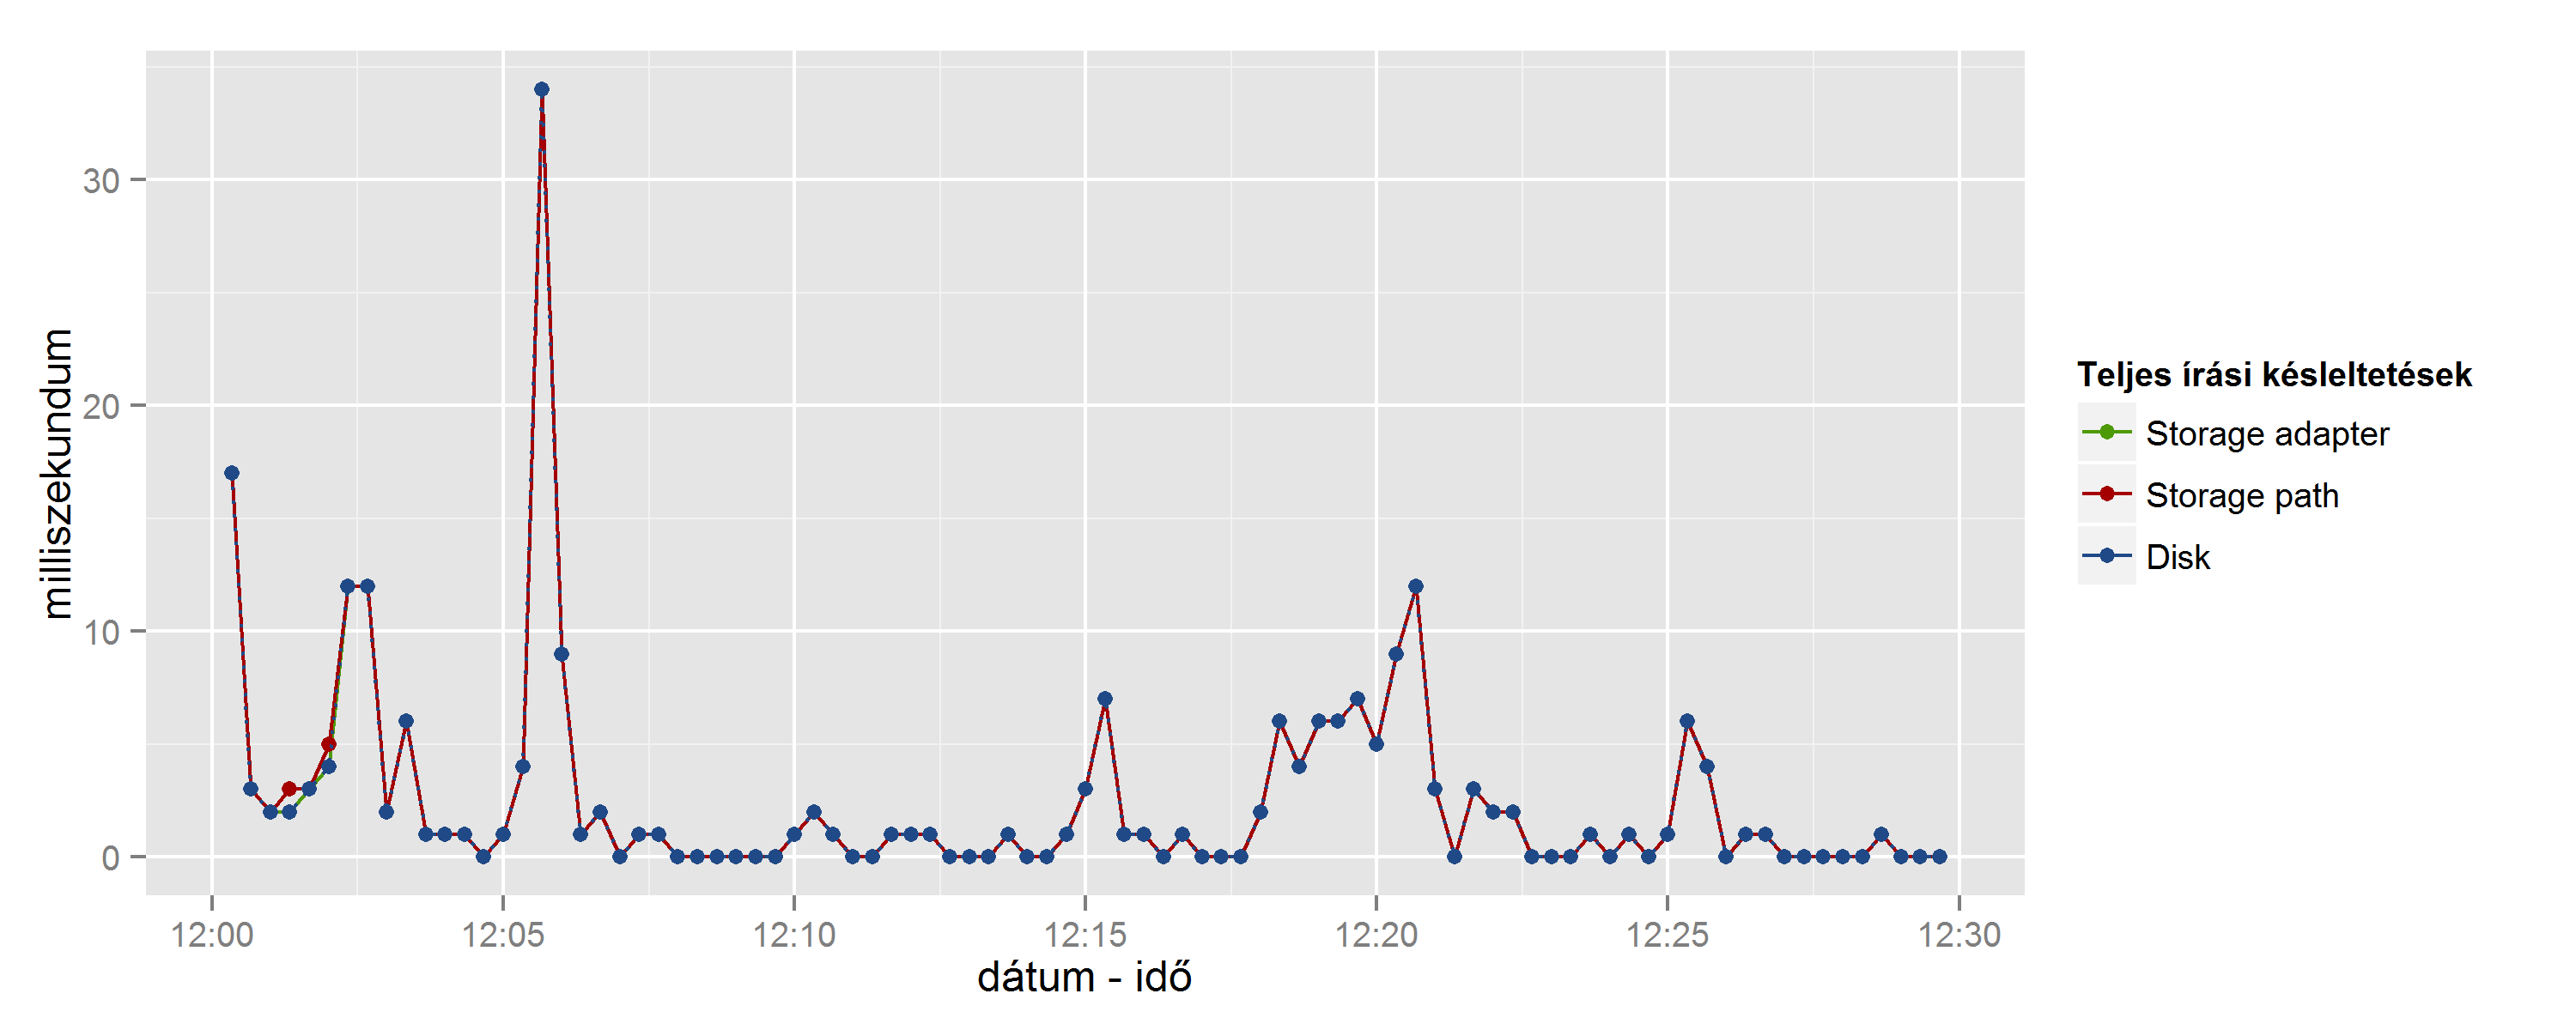
\includegraphics[width=1.00\textwidth]{figures/disk_metrics_storage_latency-20120910120000-20120910123000.png}
\caption{ Storage késleltetés a host-01 esetében 2012.09.10. 12:00:00 és 2012.09.10. 12:30:00 között \label{fig:disk_metrics_storage_latency-02}}
\end{figure}

\section{Hálózati metrikák}

\todo{Írni a hálózati metrikákról általánosan!}

\subsection{net.transmitted.average}

\todo{Megcsinálni!}

\begin{figure}[h!]
\centering
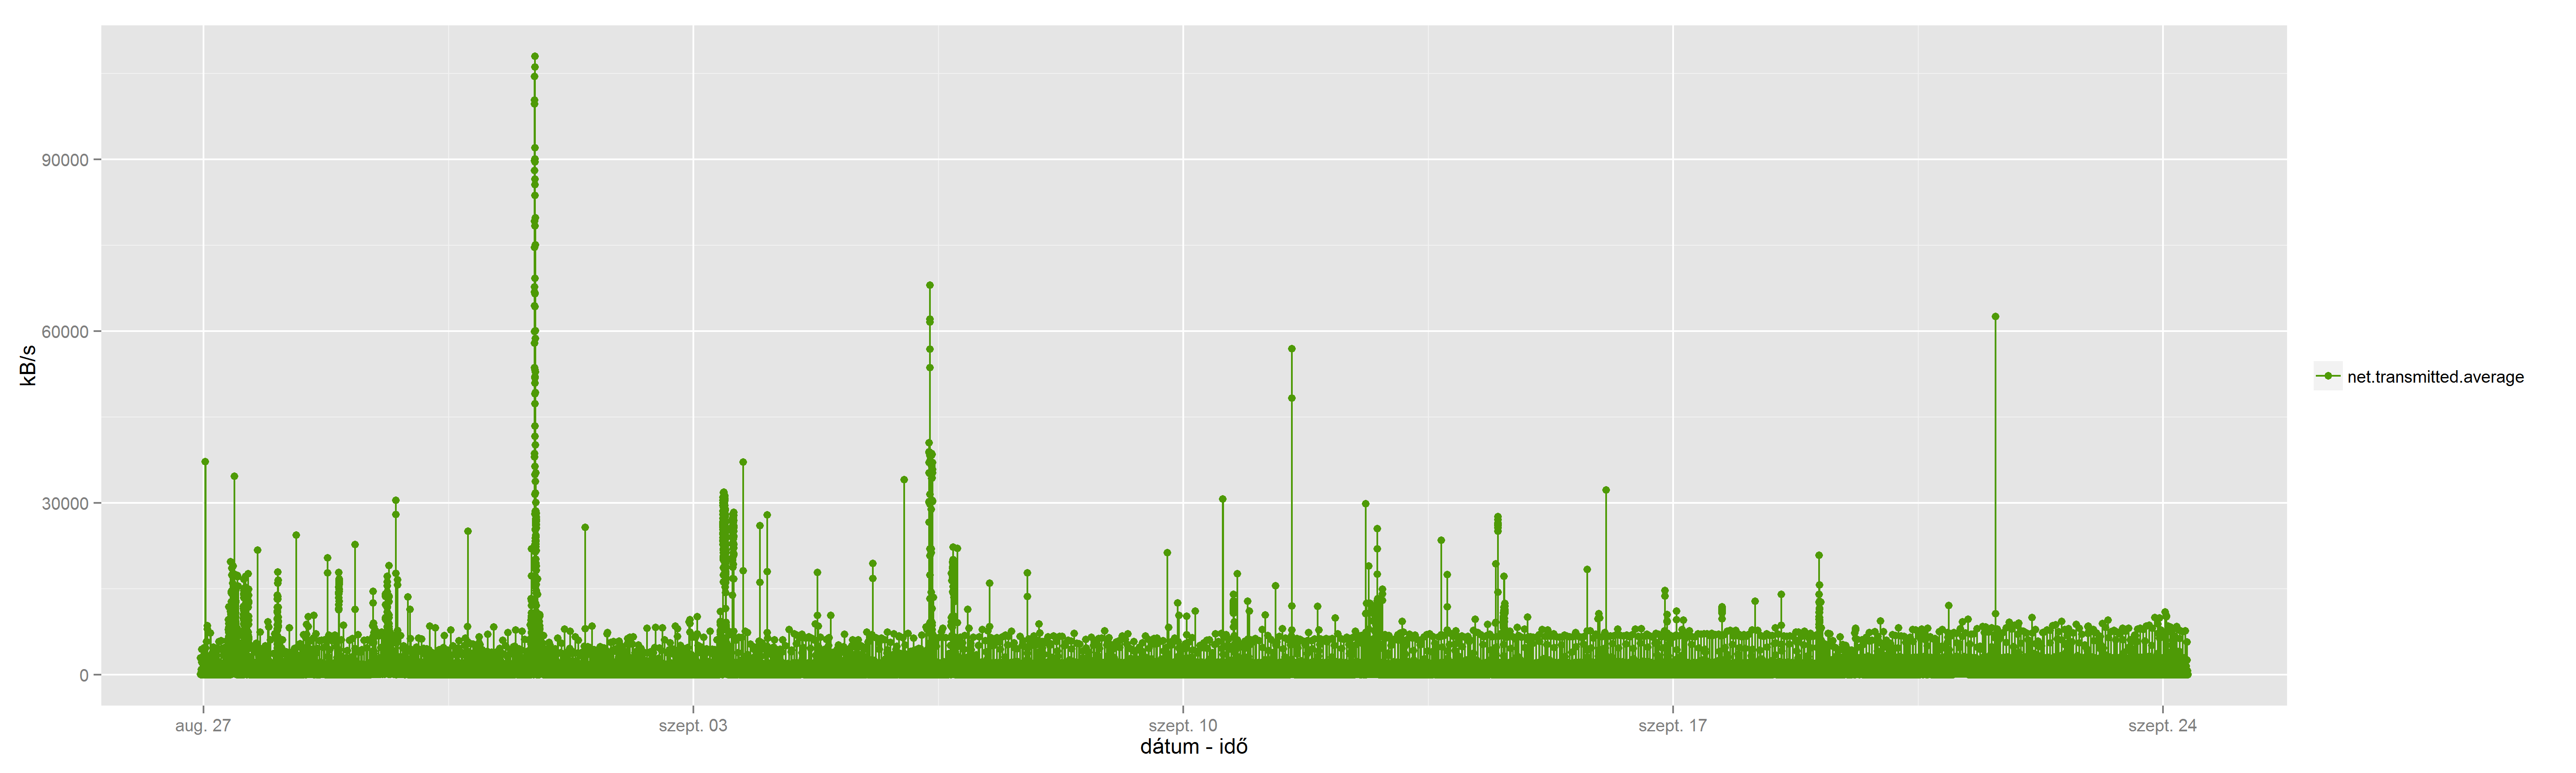
\includegraphics[width=1.00\textwidth]{figures/net_transmitted_average-20120826230140-20120924083120.png}
\caption{ A hálózati adatátviteli-sebesség alakulása a host-01 esetében a teljes megfigyelési időintervallumon \label{fig:net_transmitted_average-01}}
\end{figure}

\begin{figure}[h!]
\centering
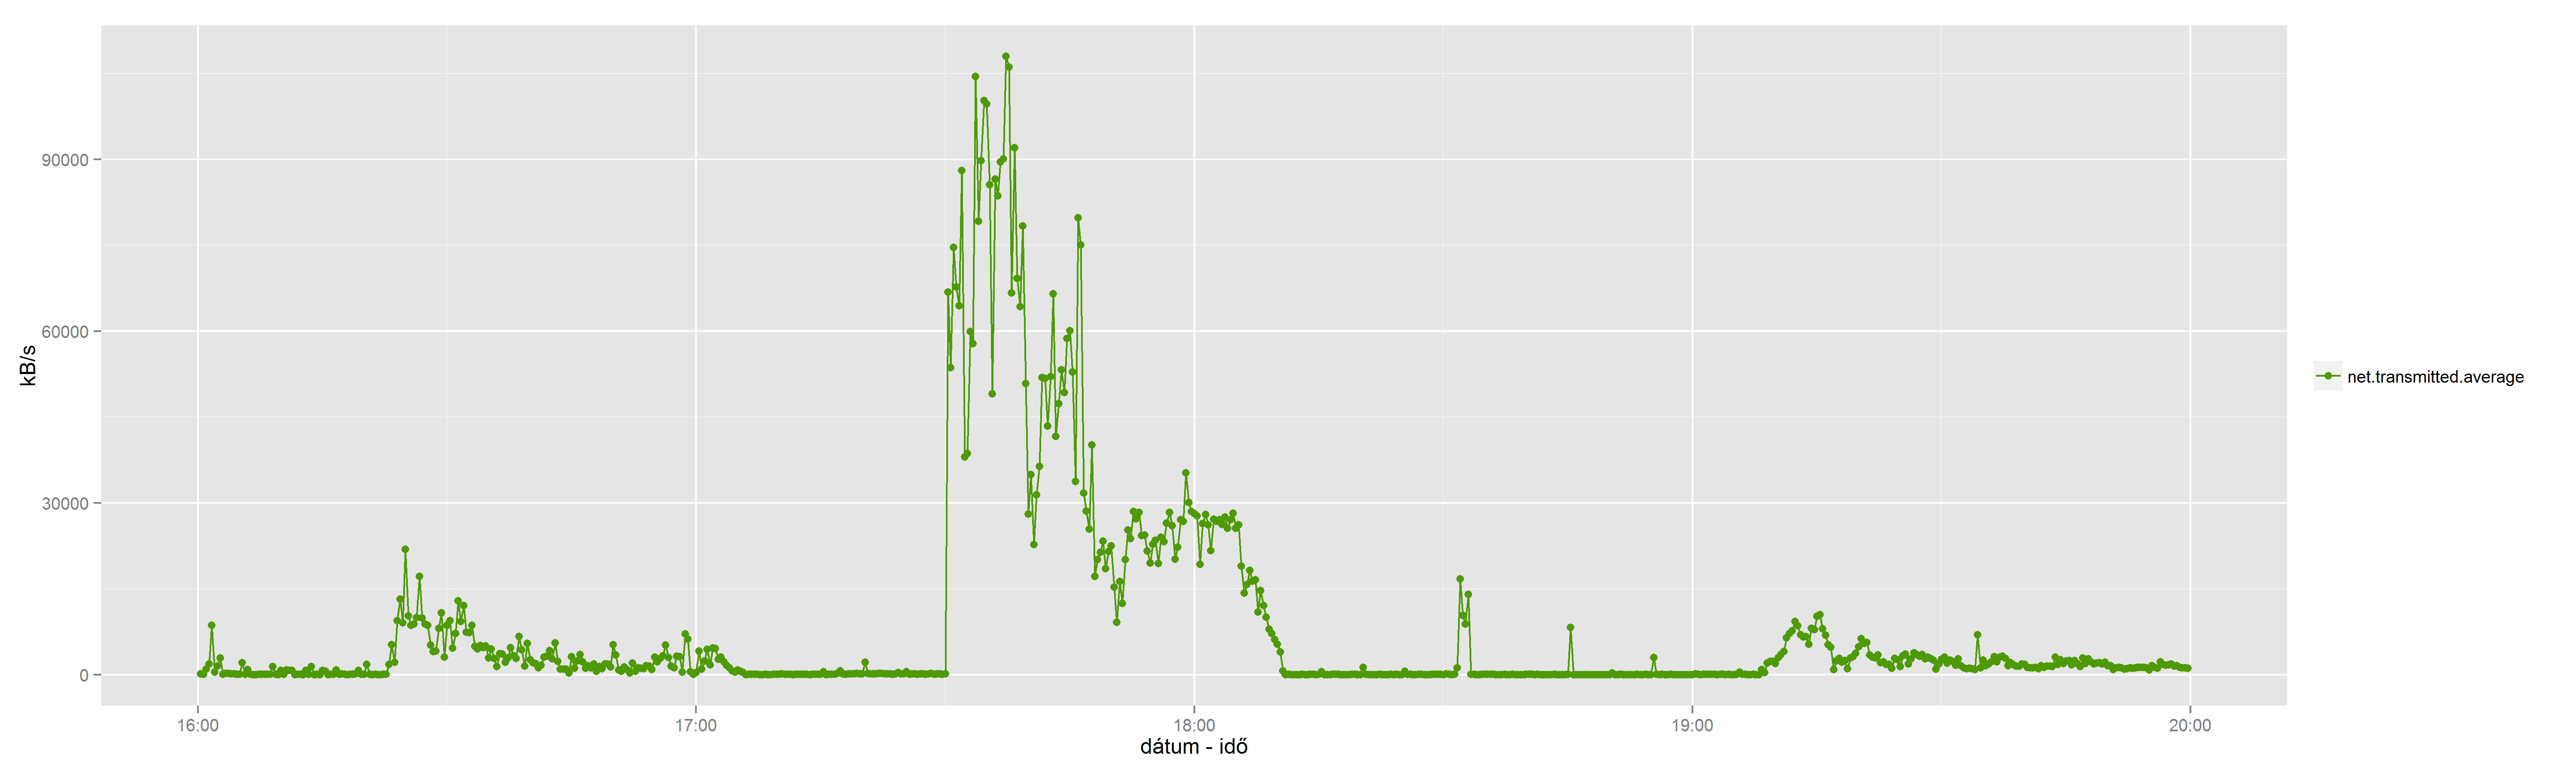
\includegraphics[width=1.00\textwidth]{figures/net_transmitted_average-20120831160000-20120831200000.png}
\caption{ A hálózati adatátviteli-sebesség alakulása a host-01 esetében 2012.08.31. 16:00:00 és 2012.08.31. 20:00:00 között \label{fig:net_transmitted_average-02}}
\end{figure}

\begin{figure}[h!]
\centering
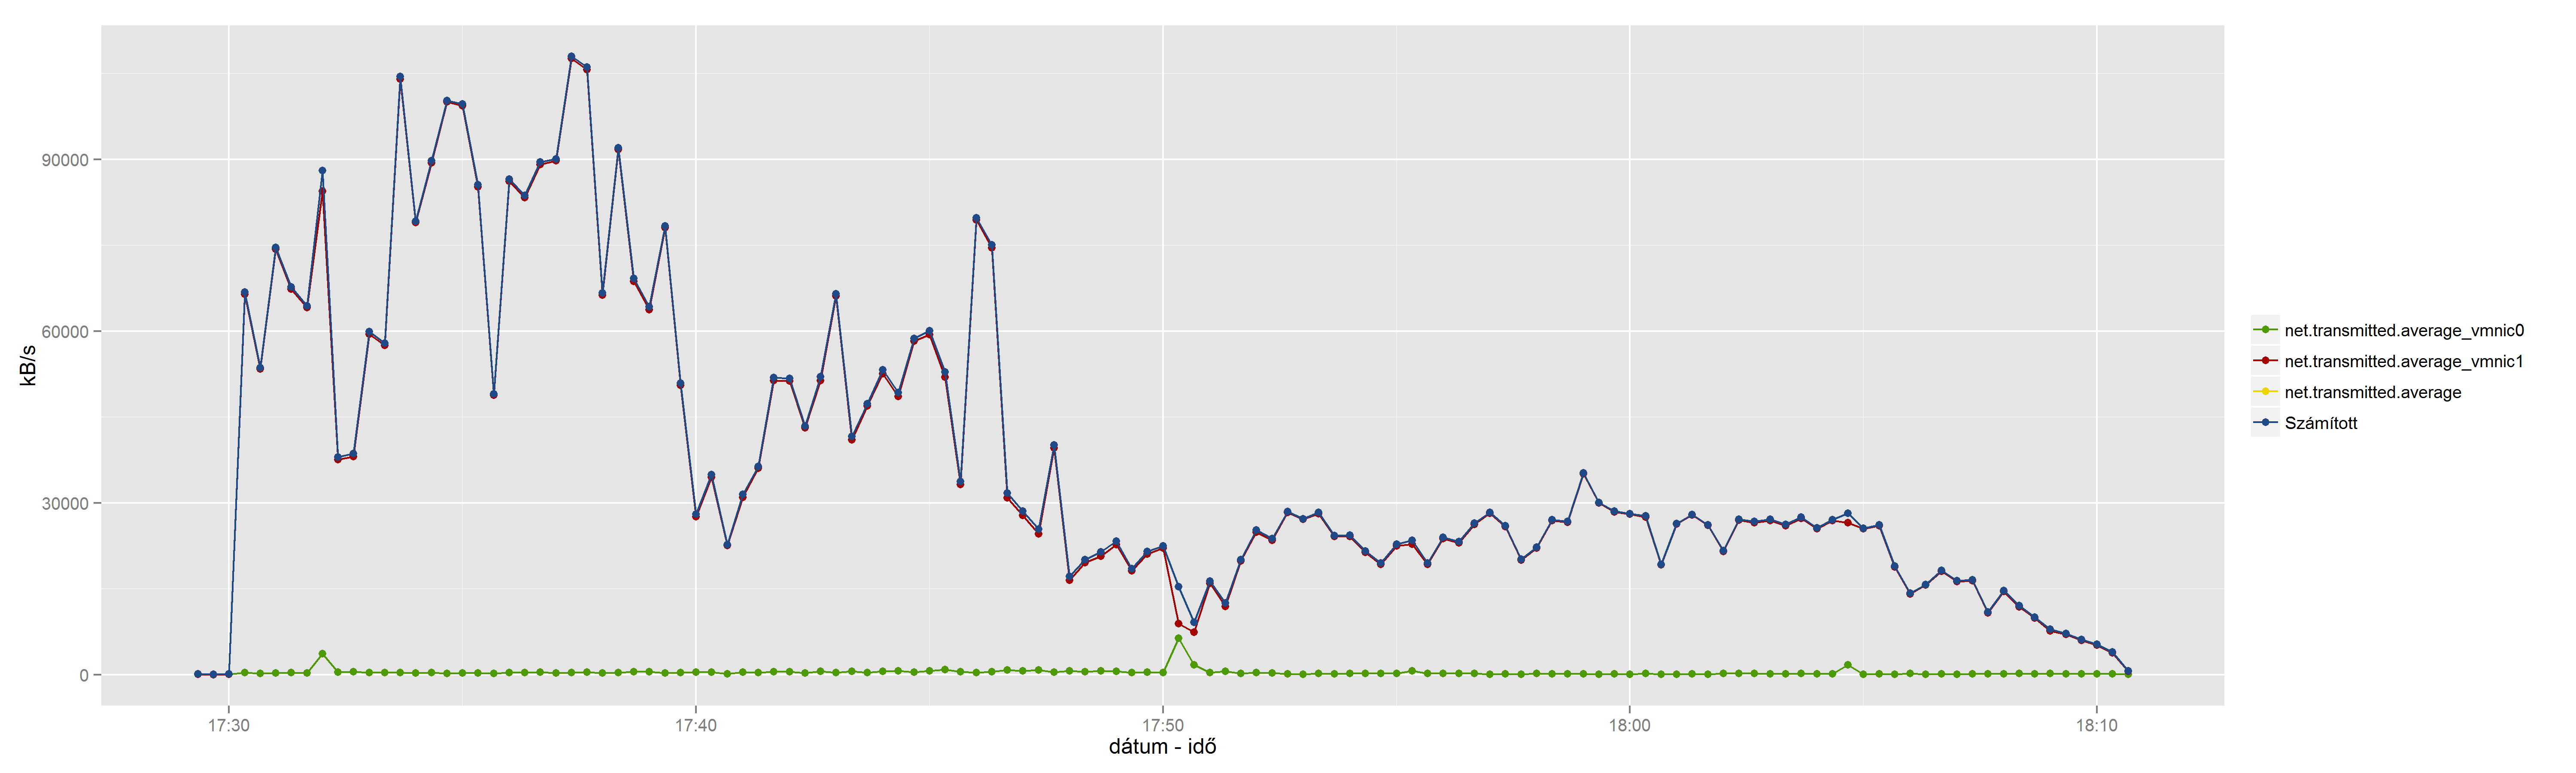
\includegraphics[width=1.00\textwidth]{figures/net_transmitted_average_dev-20120831172900-20120831181100.png}
\caption{ A hálózati adatátviteli-sebesség alakulása a host-01 esetében eszközönként 2012.08.31. 17:29:00 és 2012.08.31. 18:11:00 között \label{fig:net_transmitted_average_dev}}
\end{figure}

\begin{figure}[h!]
\centering
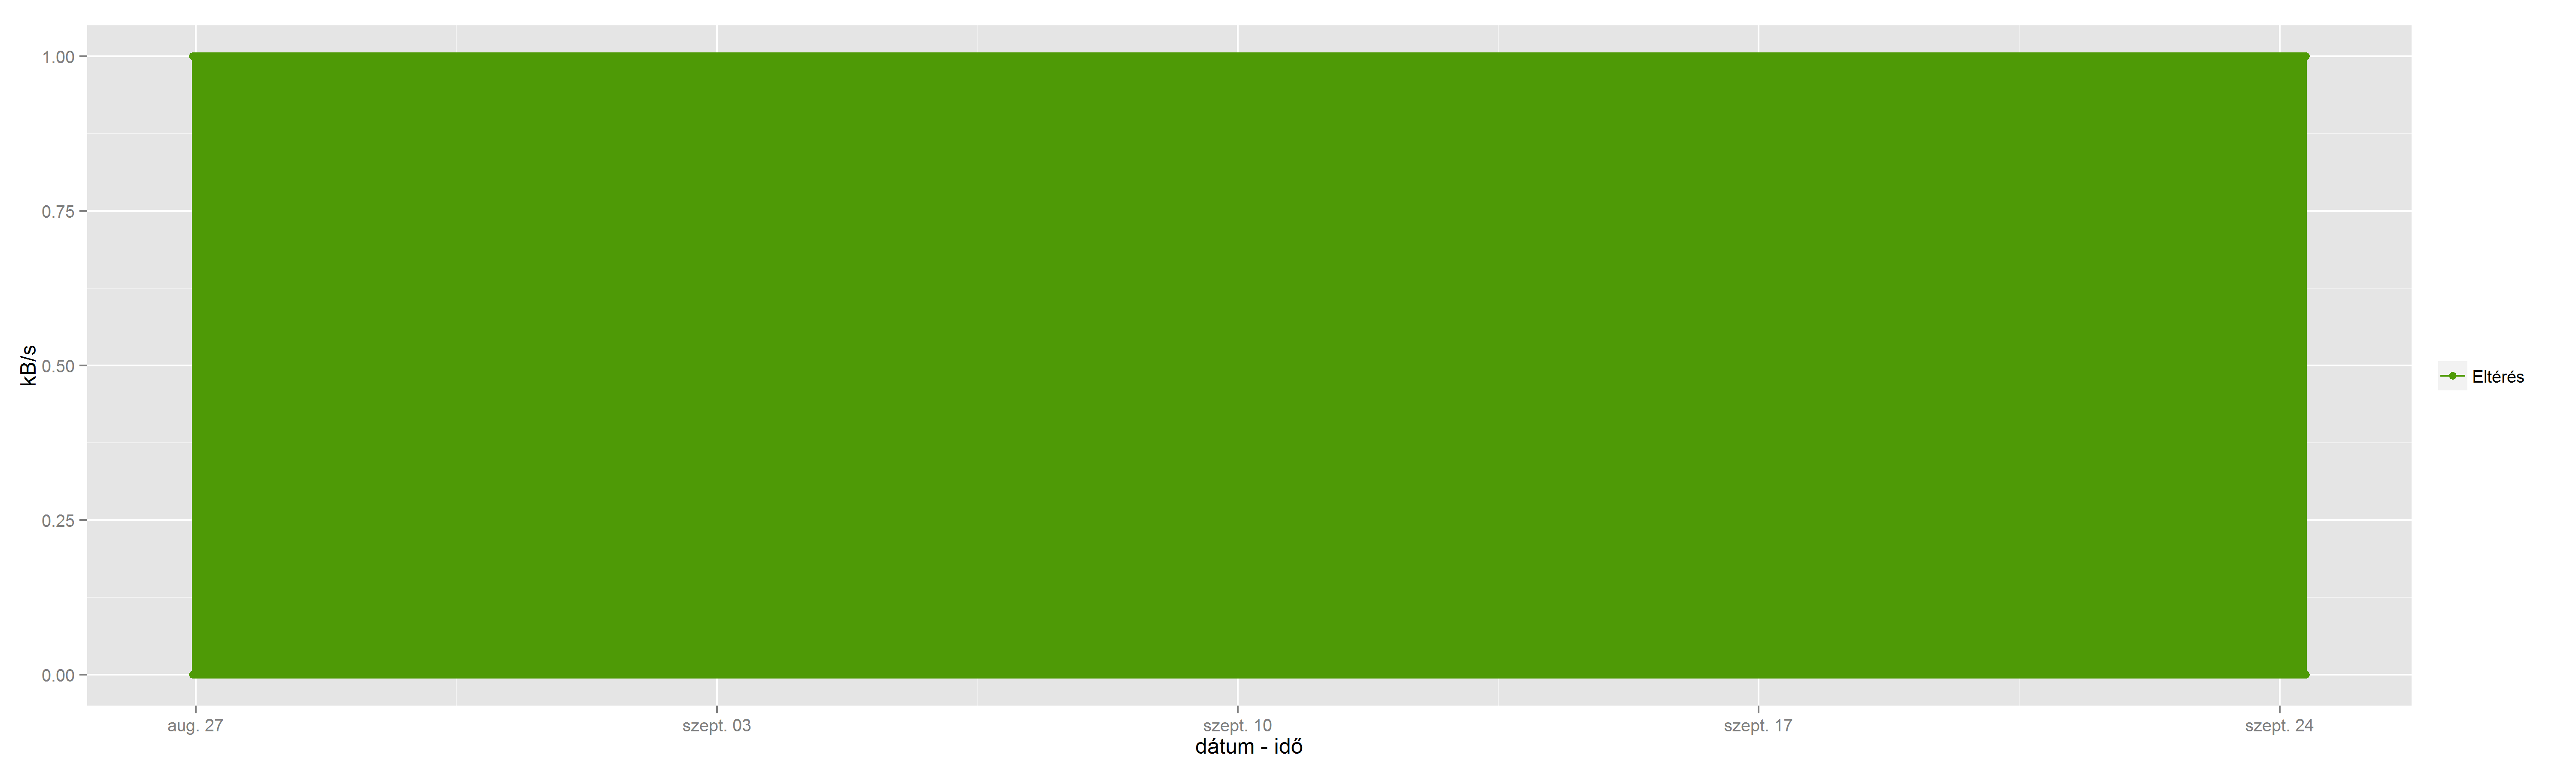
\includegraphics[width=1.00\textwidth]{figures/net_transmitted_average_diff-20120826230140-20120924083120.png}
\caption{ Eltérés a kiszámított és mért hálózati adatátviteli-sebesség között a teljes mért időintervallumon \label{fig:net_transmitted_average_diff-01}}
\end{figure}

\begin{figure}[h!]
\centering
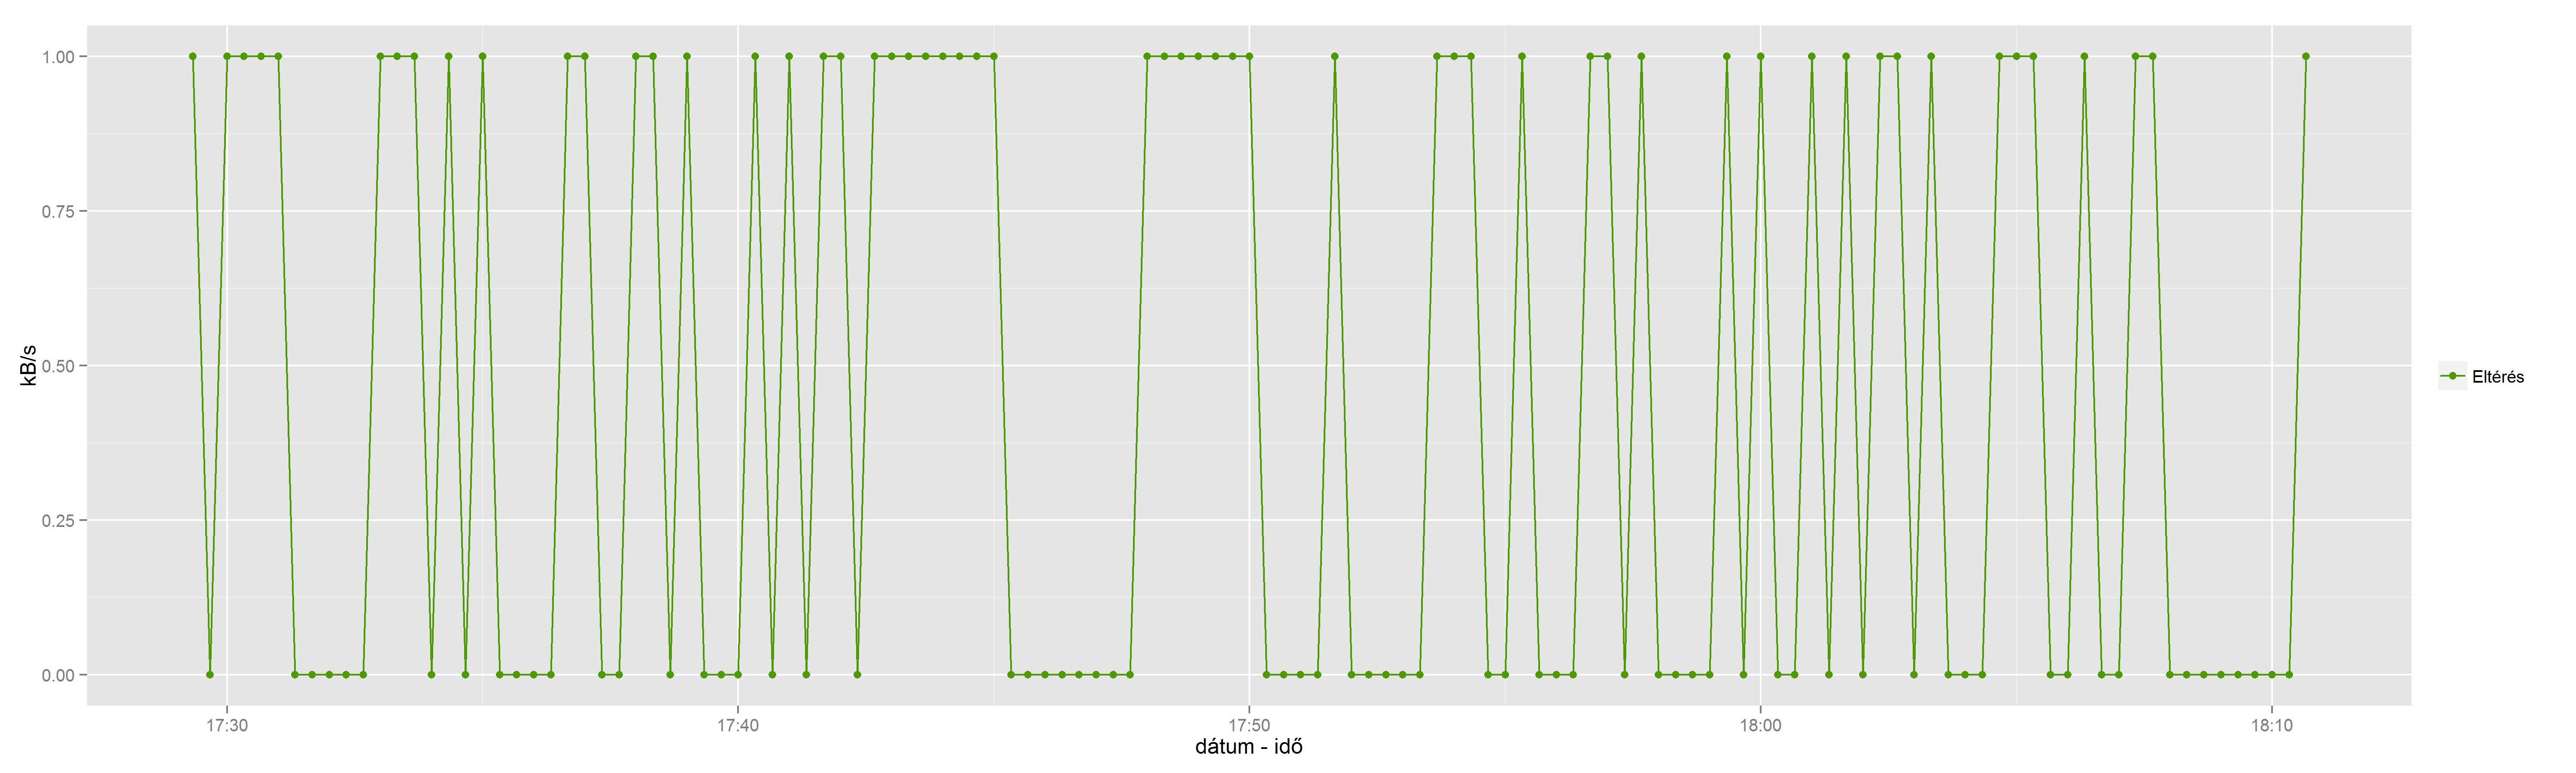
\includegraphics[width=1.00\textwidth]{figures/net_transmitted_average_diff-20120831172900-20120831181100.png}
\caption{ Eltérés a kiszámított és mért hálózati adatátviteli-sebesség között 2012.08.31. 17:29:00 és 2012.08.31. 18:11:00 között \label{fig:net_transmitted_average_diff-02}}
\end{figure}

\begin{figure}[h!]
\centering
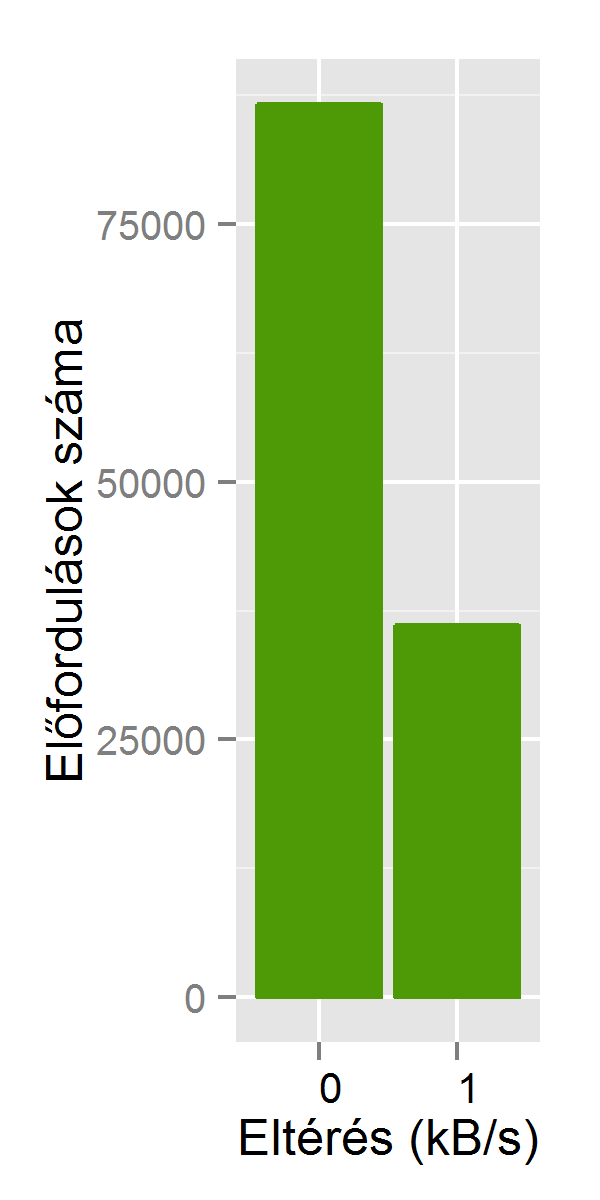
\includegraphics[width=0.25\textwidth]{figures/net_transmitted_average_diff-dist-20120826230140-20120924083120.png}
\caption{ Az eltérések eloszlása a teljes adathalmazra nézve \label{fig:net_transmitted_average_diff-dist}}
\end{figure}

%\section{Metrikák összefüggése}
%
%\todo{Megcsinálni!}

\section{Összefoglalás}

\todo{Megcsinálni!}

\section{Köszönetnyilvánítás}

A dokumentum elkészítéséhez nélkülözhetetlen segítséget nyújtott \textbf{Micskei Zoltán}, aki rendelkezésemre bocsájtotta a feldolgozásra került adathalmazt, és hasznos tanácsokkal látott el munkám során. Ezenkívül hálával tartozom \textbf{Gönczy László}nak, hogy az informatika ezen területére terelgetett.

\section{Függelék - A dokumentumban előforduló néhány metrika leírása}

\begin{table}[h]
	\caption{Néhány CPU-val kapcsolatos metrika}
	\centering
	\small
	\begin{tabular}{| p{3.5cm} | p{7.5cm} | p{2cm} |}
		\hline
		\rowcolor{tc_bone} \textbf{Metrika} & \textbf{Leírás} & \textbf{Mértékegység} \\
		\hline
		cpu.swapwait.summation & A 20 milliszekundumos ablakból mennyi időt tölt a VM várakozással (munkavégzés nélkül) amiatt, hogy nem tudja memóriába tölteni a működéséhez szükséges adatokat. & milliszekundum \\ 
		\hline
		cpu.idle.summation & A 20 milliszekundumos ablakból mennyi időt tölt a VM idle (vagyis futás nélküli) állapotban. & milliszekundum \\ 
		\hline
		cpu.ready.summation & Megmutatja, hogy egy virtuális gép az időablak hány százalékában volt olyan állapotban, hogy ugyan futásra készen állt, de nem került futtatási állapotba a fizikai processzoron. Az érték függ a virtuális gépek számától és azok CPU terheltségétől (loadjától). & milliszekundum \\ 
		\hline
		cpu.wait.summation & Értéke megadja, hogy a teljes CPU időhöz viszonyítva mennyi időt töltött a virtuális gép várakozó állapotban. & milliszekundum \\ 
		\hline
		cpu.run.summation & Megadja, hogy a VM az idő hány százalékát töltötte futási állapotban. (Származtatott érték: 100\% = run + ready + wait (+ costop) & milliszekundum \\ 
		\hline
		cpu.usage.average & Az aktívan használt virtuális CPU értéke a teljes elérhető CPU-ra nézve. Ez az átlagos kihasználtsága az összes CPU-nak az adott virtuális gépben. & \% \\ 
		\hline
		cpu.usagemhz.average & Az aktívan használt virtuális CPU értéke. Ez a host által látott CPU használat, és nem a vendég operációs rendszer által megfigyelt. & MHz \\ 
		\hline
	\end{tabular}
	\normalsize
	\label{tab:cpu.metrics}
\end{table}

\begin{table}[h]
	\caption{Néhány lemezzel kapcsolatos metrika}
	\centering
	\small
	\begin{tabular}{| p{3.5cm} | p{7.5cm} | p{2cm} |}
		\hline
		\rowcolor{tc_bone} \textbf{Metrika} & \textbf{Leírás} & \textbf{Mértékegység} \\
		\hline
		disk.deviceLatency.average &  & \\ 
		\hline
		disk.kernelLatency.average & & \\ 
		\hline
		disk.totallatency.average & & \\ 
		\hline
	\end{tabular}
	\normalsize
	\label{tab:disk.totallatency.average}
\end{table}

\todo{Lemez metrikákat megcsinálni!}

\todo{Netes metrikát megcsinálni!}

\hrulefill

\todo{Forrás: \url{http://www.slideshare.net/alanrenouf/vsphere-apis-for-performance-monitoring}}

\todo{Forrás: \url{http://www.vmware.com/support/developer/vc-sdk/}}

\todo{Forrás: \url{http://communities.vmware.com/docs/DOC-5600}}

\todo{Forrás: \url{http://communities.vmware.com/docs/DOC-5230}}

\begin{thebibliography}{99}

\bibitem[R] {link:R}
The R Project for Statistical Computing \\
Link: {\footnotesize \url{http://www.r-project.org/}}

\bibitem[GG2] {link:GG2}
ggplot2 \\
Link: {\footnotesize \url{http://ggplot2.org/}}

\bibitem[CC] {link:CC}
VMware.com - CPU Counters \\
Link: {\footnotesize \url{http://www.vmware.com/support/developer/vc-sdk/visdk400pubs/ReferenceGuide/cpu_counters.html}}

\bibitem[CRT] {link:CRT}
VMware Communities - Ready Time \\
Link: {\footnotesize \url{http://communities.vmware.com/docs/DOC-7390}}

\bibitem[VPM] {link:VPM}
Preetham Gopalaswamy, Ravi Soundararajan – VI Performance Monitoring \\
2008. szeptember 15. \\
Link: \url{http://www.vmware.com/files/webinars/communities/VI-Performance-Monitoring.pdf}

\bibitem[VMCS] {link:VMCS}
VMware vSphere 4: The CPU Scheduler in VMware ESX 4 (White paper) \\
Link: \url{www.vmware.com/files/pdf/perf-vsphere-cpu_scheduler.pdf}

\end{thebibliography}

\end{document}